\documentclass[conference]{IEEEtran}

\usepackage[numbers]{natbib}
\usepackage{graphicx}
\usepackage{amsmath}
\usepackage{amssymb}
\usepackage{amsthm}

\newtheorem{lem}{Lemma}
\newtheorem{Hyp}{Assumption}
\newtheorem{propty}{Property}
\newtheorem{thm}{Theorem}
\newtheorem{mydef}{Definition}

\usepackage{algorithm}
\usepackage{algorithmic}
\renewcommand{\algorithmicrequire}{\textbf{Input:}}
\renewcommand{\algorithmicensure}{\textbf{Output:}}

\usepackage{subfigure}
\usepackage{float}

\begin{document}

\title{Informative Path Planning with a Human Path Constraint}

\author{
\IEEEauthorblockN{Daqign Yi, Michael A. Goodrich and Kevin D. Seppi}
\IEEEauthorblockA{Department of Computer Science\\
Brigham Young University\\
Provo, Utah 84604\\
Email: daqing.yi@byu.edu, \{mike, kseppi\}@cs.byu.edu}
}

\maketitle

\begin{abstract}
One way for a human and a robot to collaborate on a search task is for the human to specify constraints on the robot's path and then allow the robot to find an optimal path subject to these constraints.
This paper presents an anytime solution to the robot's path-planning problem when the human specifies a path constraint and an acceptable amount of deviation from this path.
The robot's objective is to maximize information gathered during the search subject to this constraint.
We first discretize the path constraint and then convert the resulting problem into a multi-partite graph.
Information maximization becomes a submodular orienteering problem on this topology structure.
Backtracking is used to generate an efficient heuristic for solving this problem, and an expanding tree is used to facilitate an anytime algorithm.
\end{abstract}

\IEEEpeerreviewmaketitle

\section{Introduction}

\begin{frame}{Modeling human intent}{Path Planning}
THe problem in modeling human intent
\begin{itemize}
\item incomparability in objectives
\item conflict in objectives
\item hardness in weighing the objectives
\item vagueness in importance selection
\end{itemize}
\begin{figure}
\centering
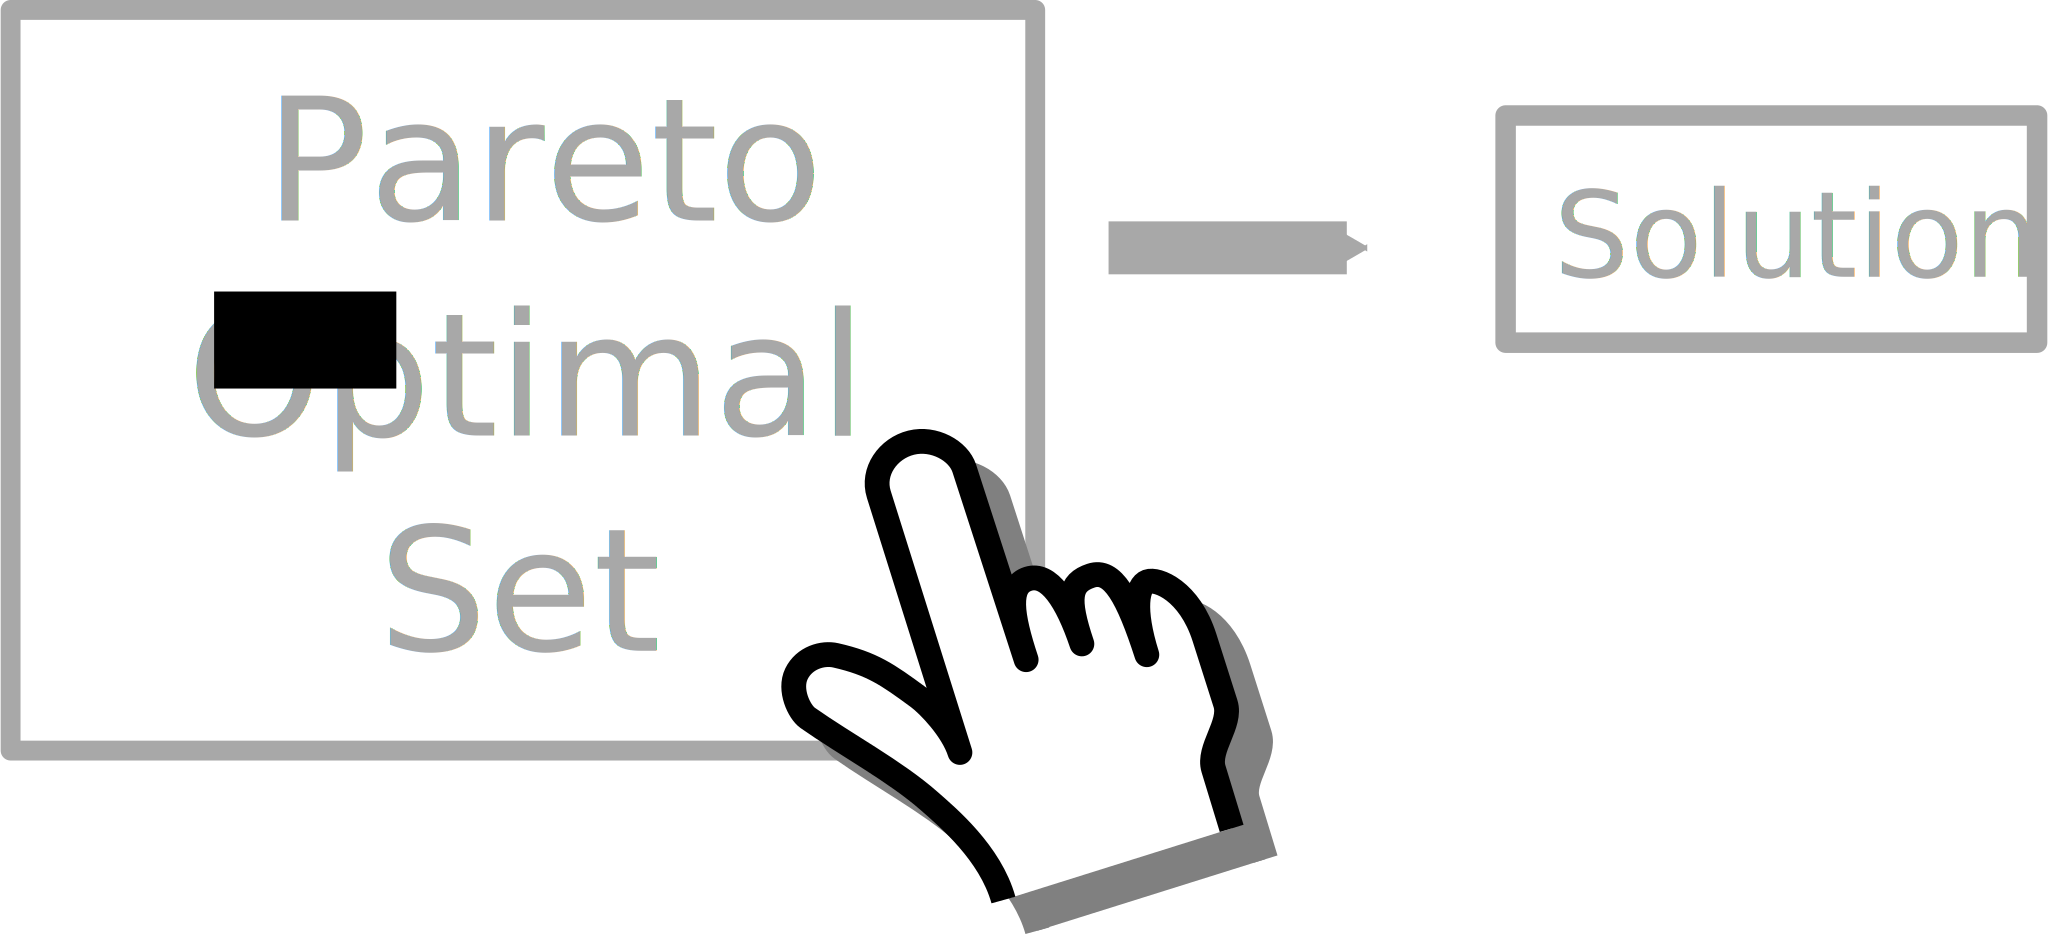
\includegraphics[width=0.6\linewidth]{figure/human_interactive_moo}
%\caption{}
\label{fig:human_interactive_moo}
\end{figure}
\end{frame}

\begin{frame}{Pareto Optimal}{}
\end{frame}

\section{Problem definition}

\subsection{Informative path}

\begin{frame}{Coverage model}{Informative path}

\begin{itemize}
\item Information measurement - entropy 
\item Maximum coverage problem
\end{itemize}

\begin{figure}
\centering
\includegraphics[width = 0.6\textwidth]{./figure/robotObservation}
%\caption{A coverage model.}
\end{figure}

\end{frame}

\begin{frame}{Submodularity}{Informative path}

\begin{columns}

\column{0.45\textwidth}

\begin{figure}
\centering
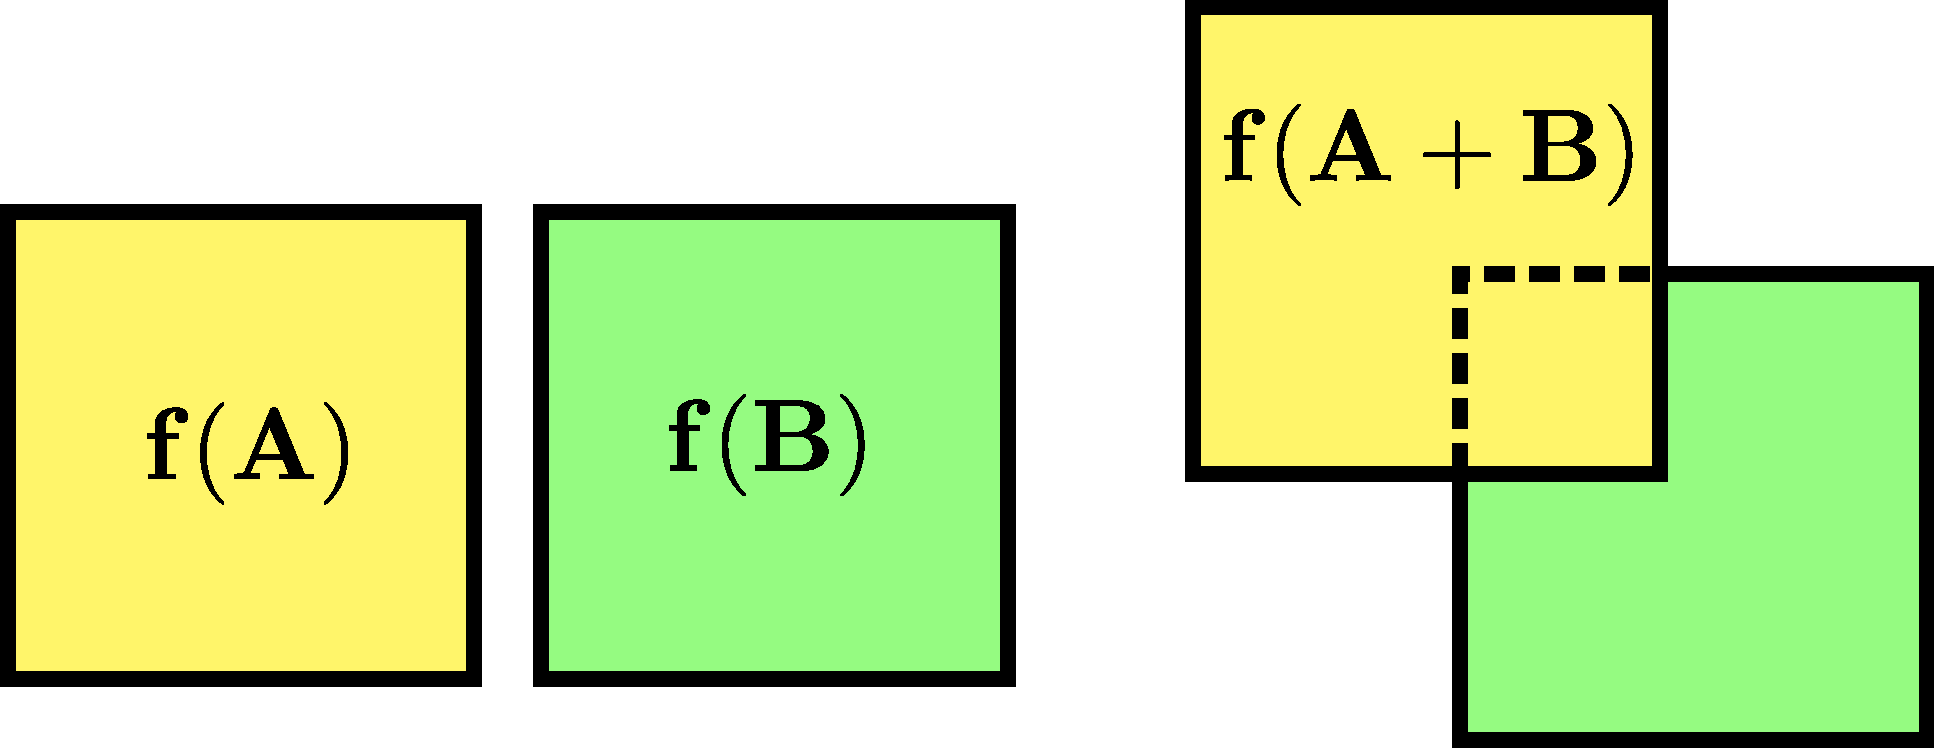
\includegraphics[width = \textwidth]{./figure/submodular}
%\caption{A coverage model.}
\end{figure}

\begin{equation}
\nonumber
f(A) + f(B) \geq f(A+B)
\end{equation}

\column{0.1\textwidth}

\column{0.45\textwidth}

Information
\begin{itemize}
\item search space $ S $
\item the observation of a robot $ \mathbf{O}^{X} $ 
\item the observation of a human $ \mathbf{O}^{Y} $

\bigskip
\bigskip

$ f( \mathbf{S}, \mathbf{O}^{X} ) + f( \mathbf{S}, \mathbf{O}^{Y^{h}} ) \geq f( \mathbf{S}, \mathbf{O}^{X},  \mathbf{O}^{Y^{h}} ) $ 
\end{itemize}

\end{columns}

\end{frame}

\begin{frame}{Submodular orienteering}{Informative path}

\begin{block}{Conditional mutual information}
$ I(\mathbf{S}; \mathbf{O}^{X} \mid \mathbf{O}^{Y^{h}}) = H(\mathbf{S} \mid \mathbf{O}^{Y^{h}}) - H(\mathbf{S} \mid \mathbf{O}^{X},\mathbf{O}^{Y^{h}}) $
\end{block} 

\bigskip

\begin{itemize}
\item Entropy reduction
\item Submodularity
\item Chain rule \\
$ I(\mathbf{S}; \mathbf{O}^{X} \mid \mathbf{O}^{Y^{h}}) = \sum_{t=1}^{T} I(O^{X}_{t} ; \mathbf{S} \mid O^{X}_{1} , \cdots , O^{X}_{t-1}, \mathbf{O}^{Y^{h}}) $
\end{itemize}

\end{frame}

\subsection{Human constraint}

\begin{frame}{Team role}{Human constraint}

\begin{figure}
\centering
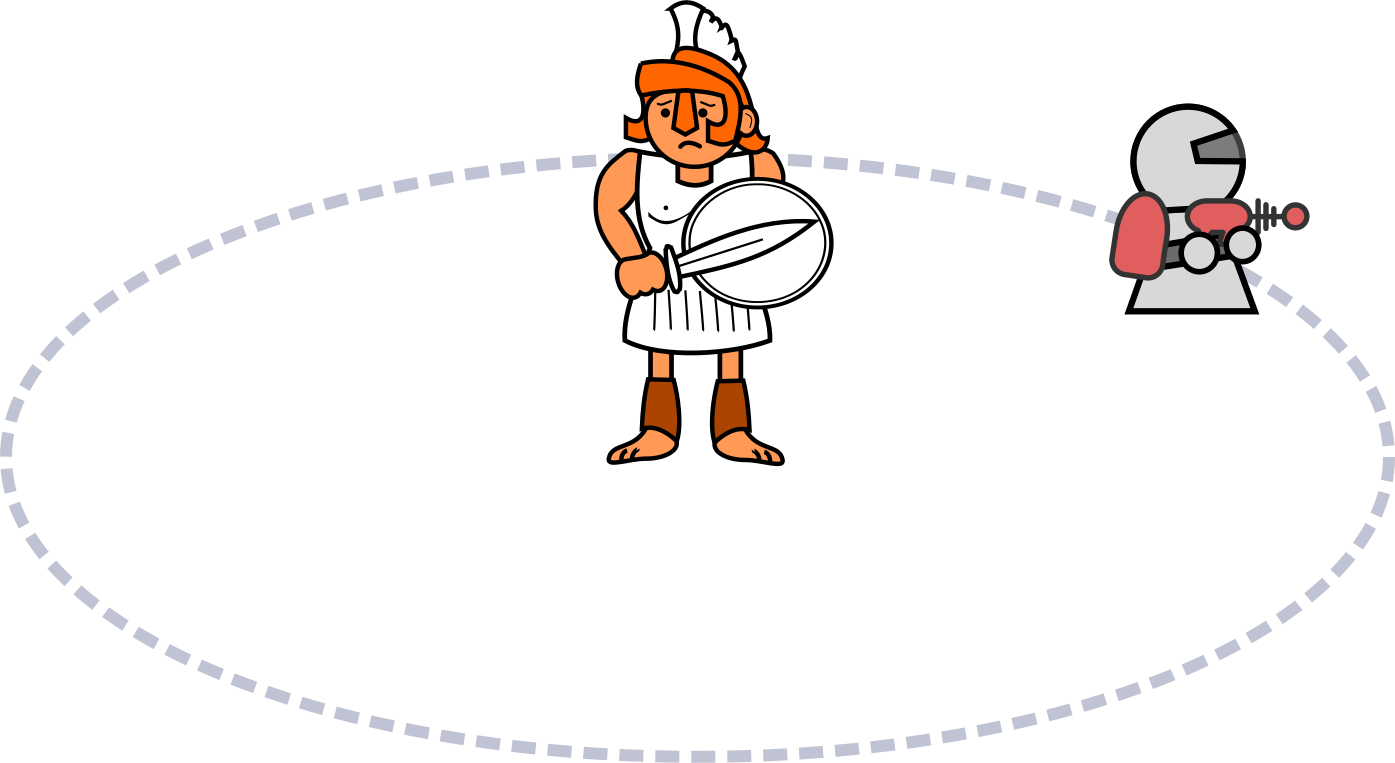
\includegraphics[width = 0.7\textwidth]{./figure/human_robot_interaction}
\end{figure}

\begin{itemize}
\item cooperative observation
\item assistance and protection
\end{itemize}

\end{frame}

\begin{frame}{Neighboring function}{Human constraint}

\begin{columns}
\column{.6\linewidth}
\begin{minipage}[c]{\linewidth}
\begin{figure}
\centering
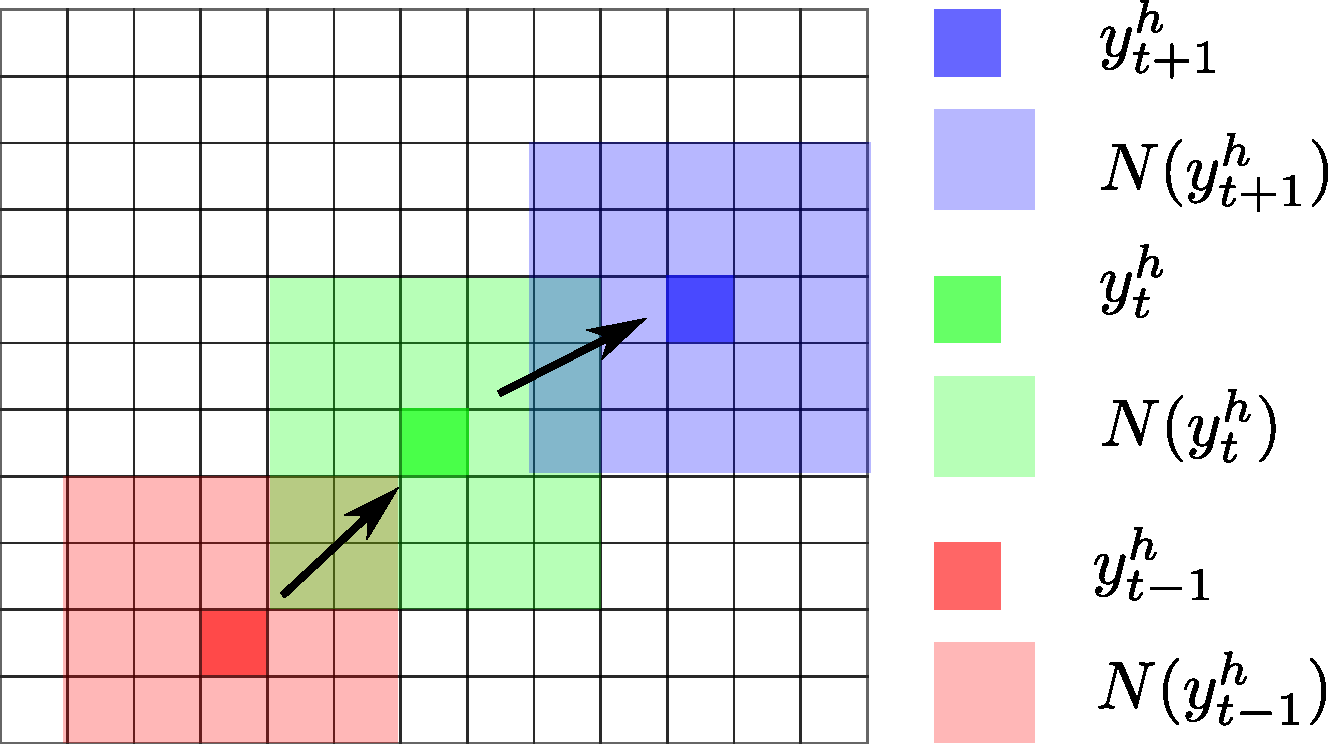
\includegraphics[width = \textwidth]{./figure/humanConstraint}
%\caption{An example of human constraint.}
\end{figure}
\end{minipage}

\column{.4\linewidth}
\begin{minipage}[c]{\linewidth}
\begin{itemize}
\item { human path $ \{ y^{h}_{1} \cdots y^{h}_{T} \} $ }
\item { neighboring function $ N( y^{h}_{t} ) $ }
\end{itemize}
\end{minipage}
\end{columns}

\end{frame}

\subsection{The optimization model}

\begin{frame}{Problem abstraction}{The optimization model}

\begin{figure}
\centering
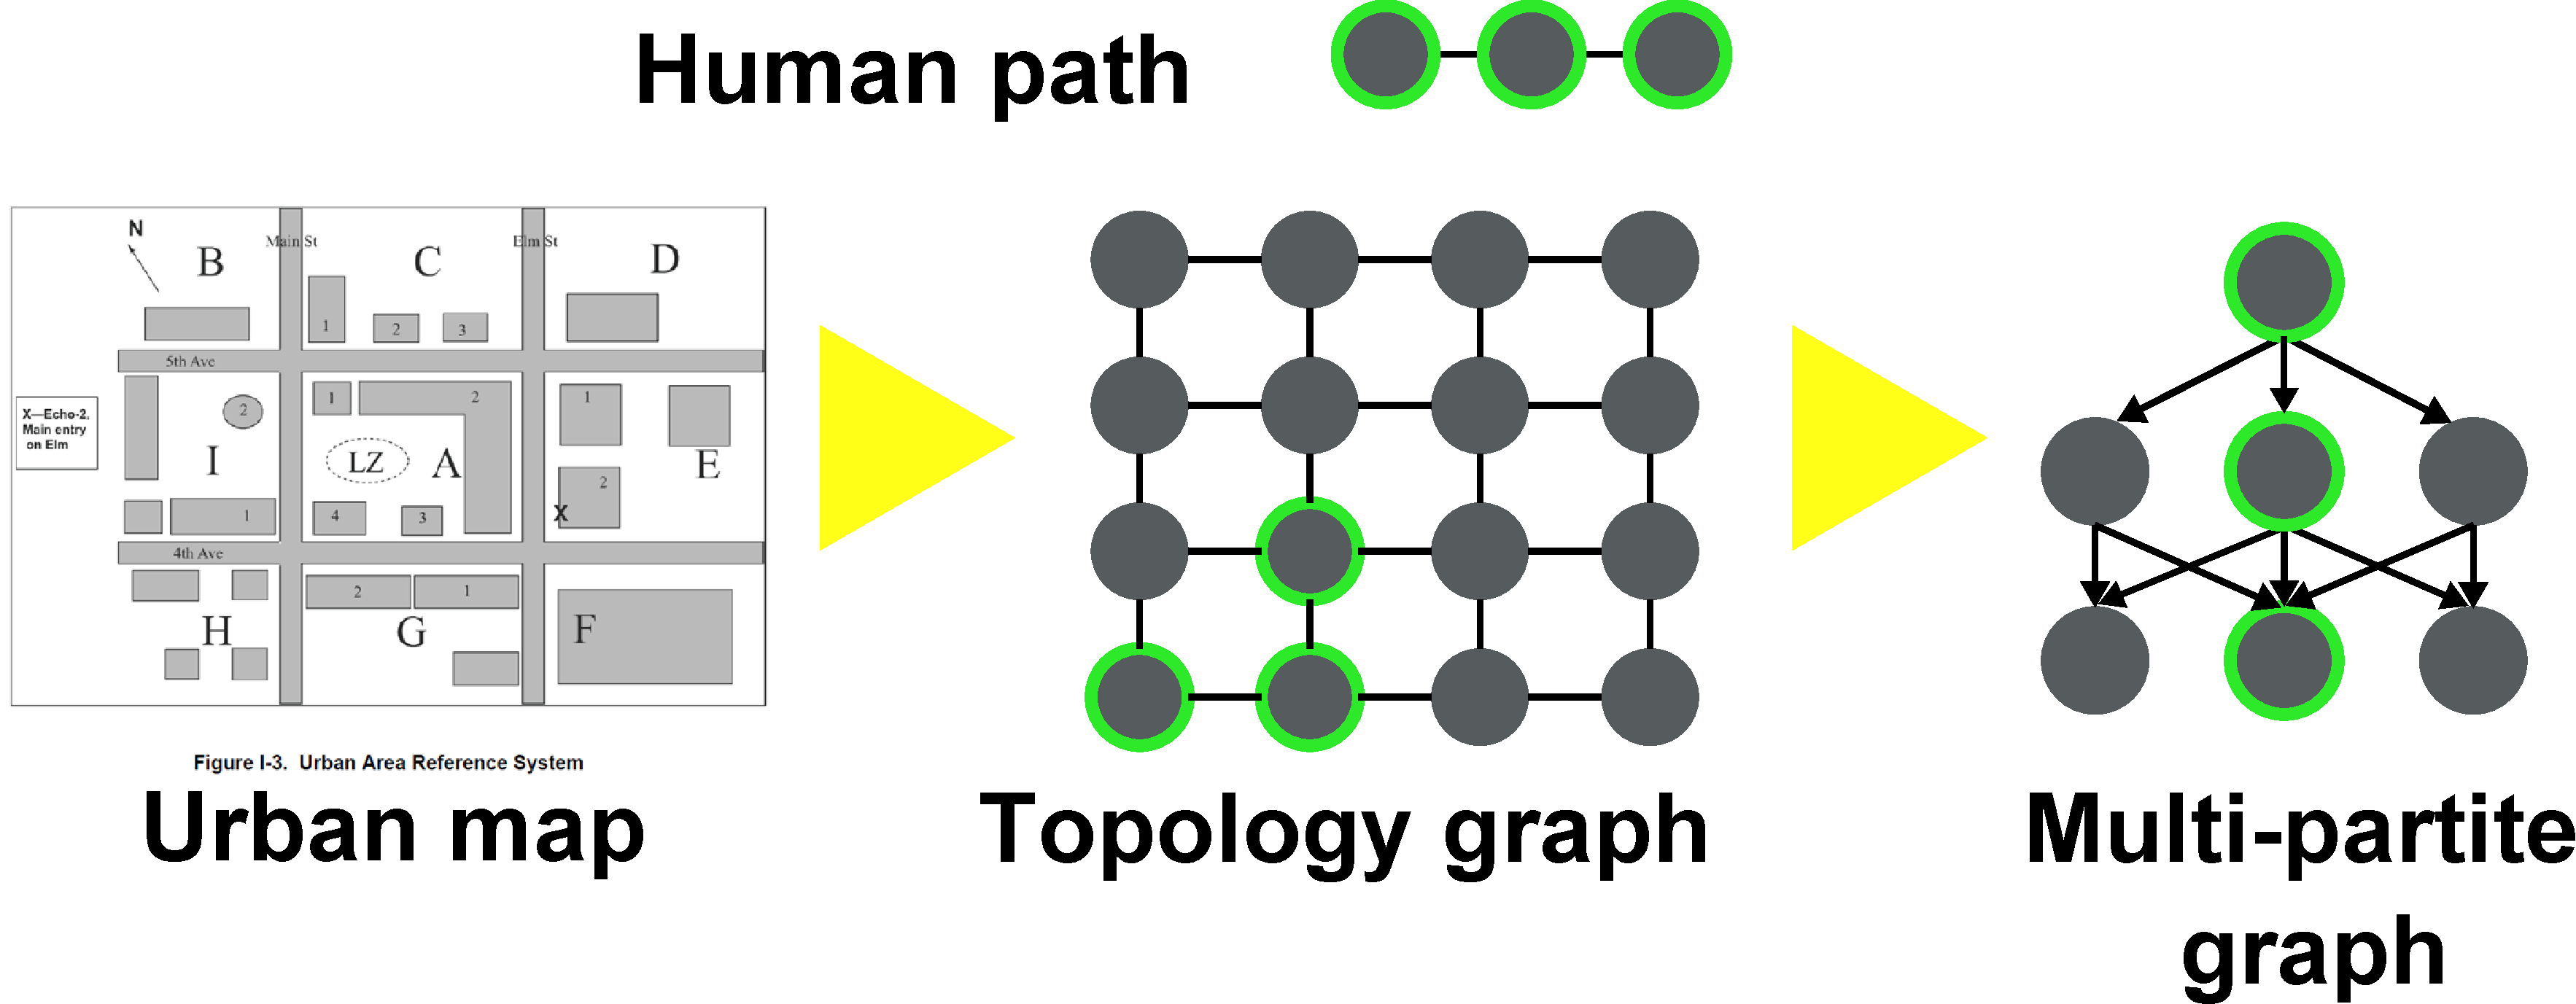
\includegraphics[width = 0.9\textwidth]{./figure/layers}
%\caption{A layered problem processing.}
\end{figure}

\end{frame}

\begin{frame}{The multi-partite graph}{The optimization model}

\begin{columns}

\column{.6\textwidth}
\begin{minipage}[c]{\textwidth}
\begin{figure}
\centering
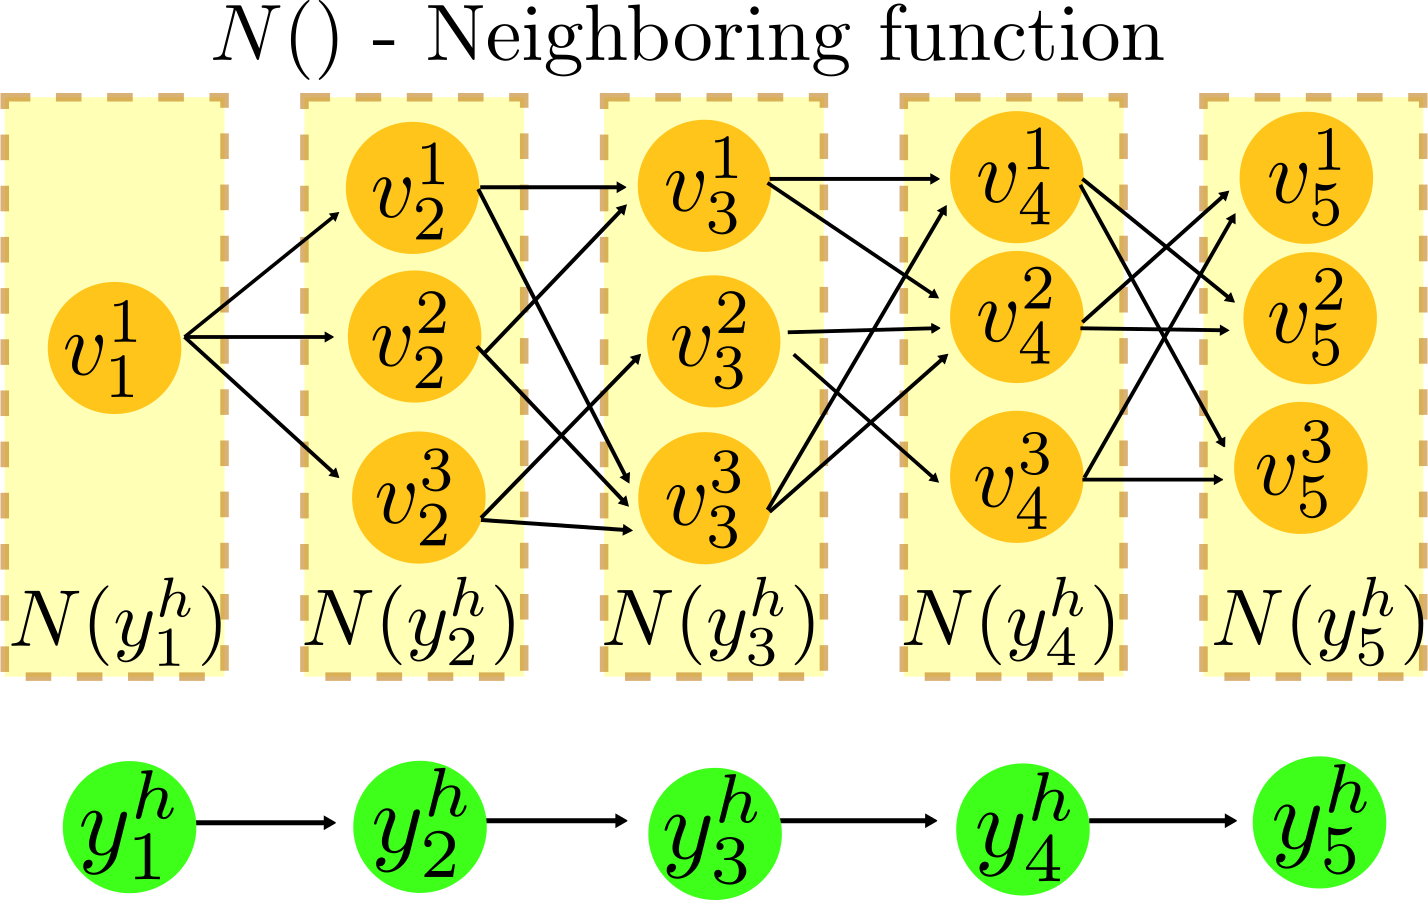
\includegraphics[width = \textwidth]{./figure/MultiPartite}
%\caption{A multi-partite graph generated from human constraint.}
\end{figure}
\end{minipage}

\column{.4\textwidth}
\begin{minipage}[c]{\textwidth}
\begin{itemize}
\item time-space synchronization
\item connection determined by discretized map
\end{itemize}
\end{minipage}

\end{columns}

\end{frame}

\begin{frame}{A pruning process}{The optimization model}

\begin{columns}
\column{.45\textwidth}
%\begin{minipage}
%\begin{block}
Reachable
%\end{block}
%\end{minipage}

\column{.45\textwidth}
%\begin{minipage}
%\begin{block}
Non-terminating
%\end{block}
%\end{minipage} 

\end{columns}

\begin{columns}

\column{.45\textwidth}

\begin{block}{Forward pruning}
$ \forall t \in \{ 2, \cdots T \}, $ \\
$ \forall v \in V(t), deg^{-}(v) > 0 $

\begin{figure}
\centering
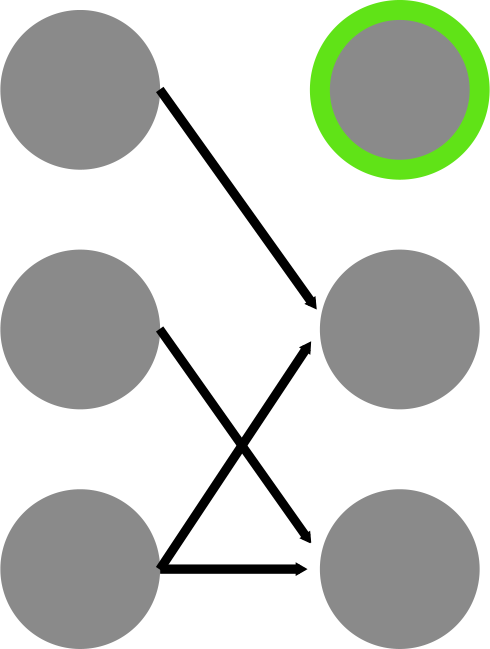
\includegraphics[width = 0.4\textwidth]{./figure/forward_prune}
\end{figure}

\end{block}

\column{.45\textwidth}

\begin{block}{Backward pruning}

$ \forall t \in \{ 1, \cdots T-1 \}, $ \\
$ \forall v \in V(t), deg^{+}(v) > 0 $

\begin{figure}
\centering
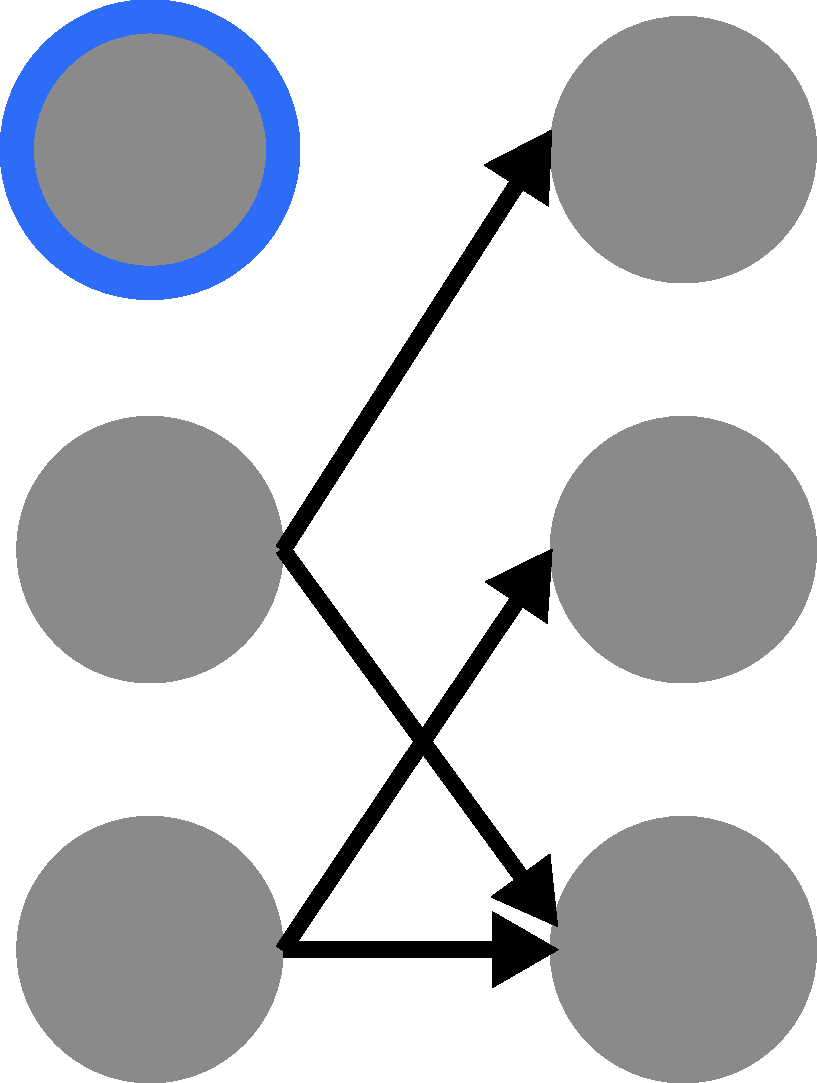
\includegraphics[width = 0.4\textwidth]{./figure/backward_prune}
\end{figure}

\end{block}

\end{columns}

\end{frame}

\begin{frame}{Obstacles}{The optimization model}

\begin{figure}
\centering
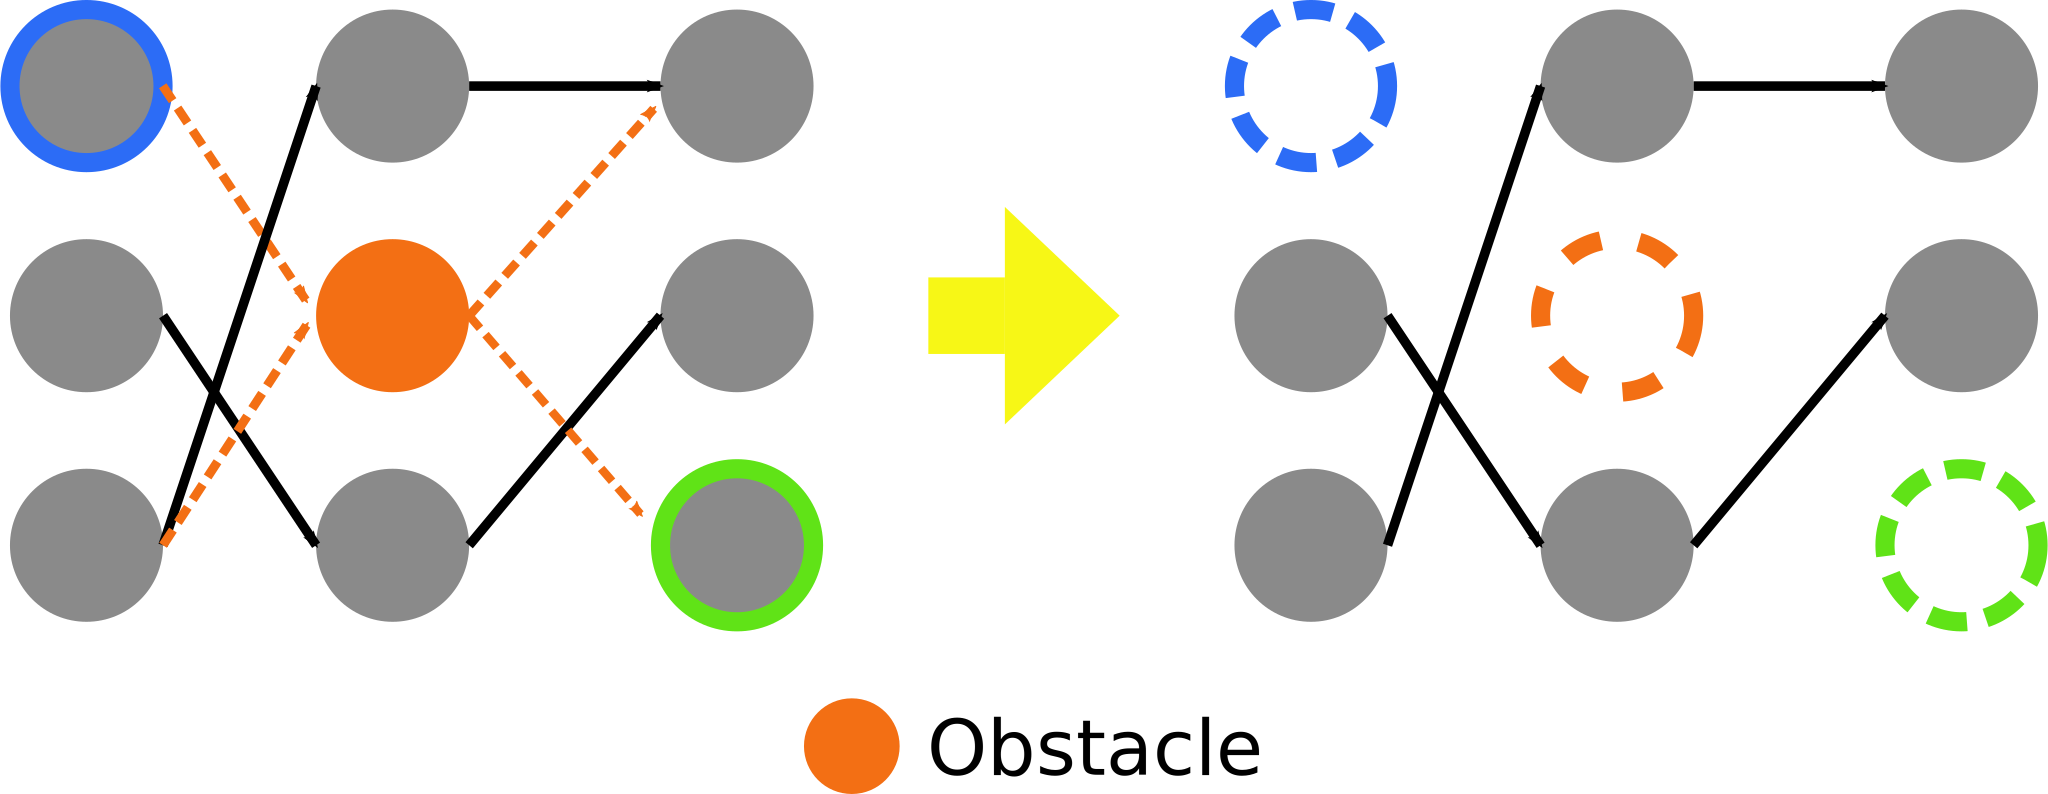
\includegraphics[width = 0.8\textwidth]{./figure/obstacle}
\end{figure}

\end{frame}

\begin{frame}{Submodular orienteering on a multi-partite graph}{The optimization problem}

\begin{equation}
\nonumber
\begin{aligned}
Objective: & X^{*} = \argmax_{X} \: f(X); \\
Constraint: & |X| = T, x_{t} \in V(t), (x_{t}, x_{t+1}) \in E.
\end{aligned}
\end{equation}

\end{frame}



\section{Solution}

\subsection{Backtracking heuristic}

\begin{frame}{Bellman-like equation}{Heuristic}

%\begin{equation}
%\nonumber
%\hat{x}_{t} = \argmax_{X_{t}} [ f(x_{t} \mid x_{1} , \cdots , x_{t-1}) + \max_{X_{t+1}, \cdots , X_{T}} f(x_{t+1}, \cdots , x_{T} \mid x_{1}, \cdots , x_{t}) ]
%\end{equation}

\centering
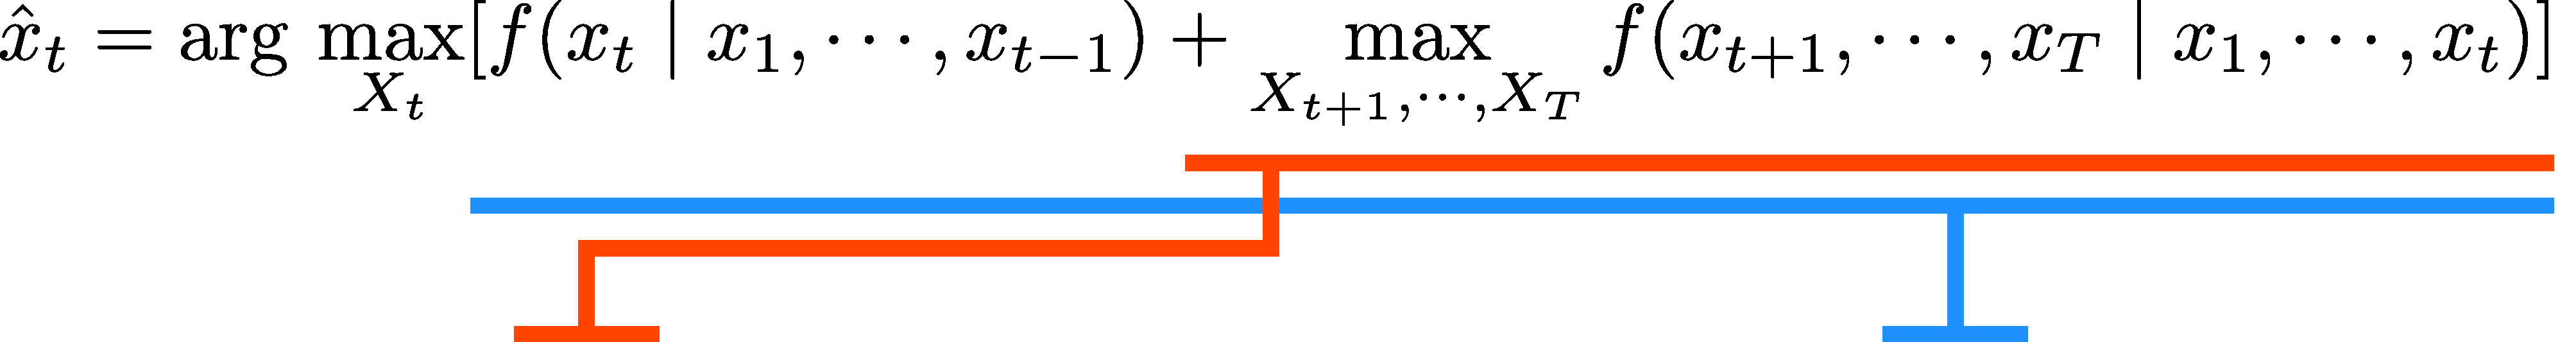
\includegraphics[width = \textwidth]{./figure/arg_equation}

\begin{columns}
\column{0.45\textwidth}
\begin{block}{Maximum future reward}
\begin{figure}
\centering
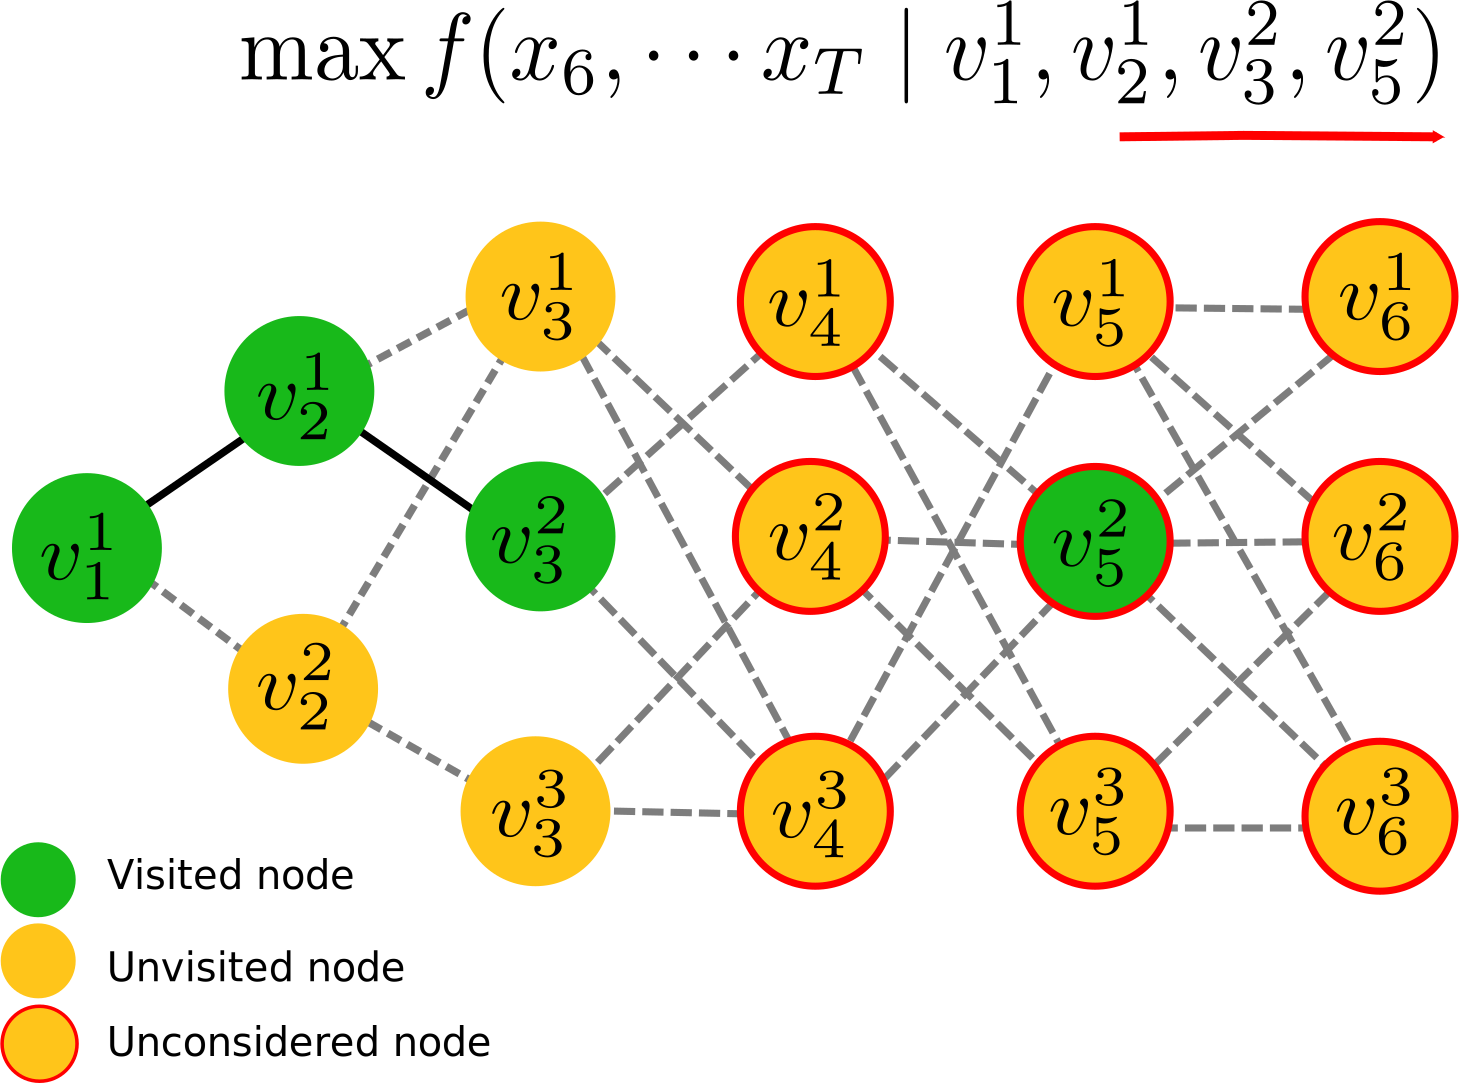
\includegraphics[width = 0.9\textwidth]{./figure/DefineFuncH}
\end{figure}
\end{block}

\column{0.45\textwidth}
\begin{block}{Maximum total reward}
\begin{figure}
\centering
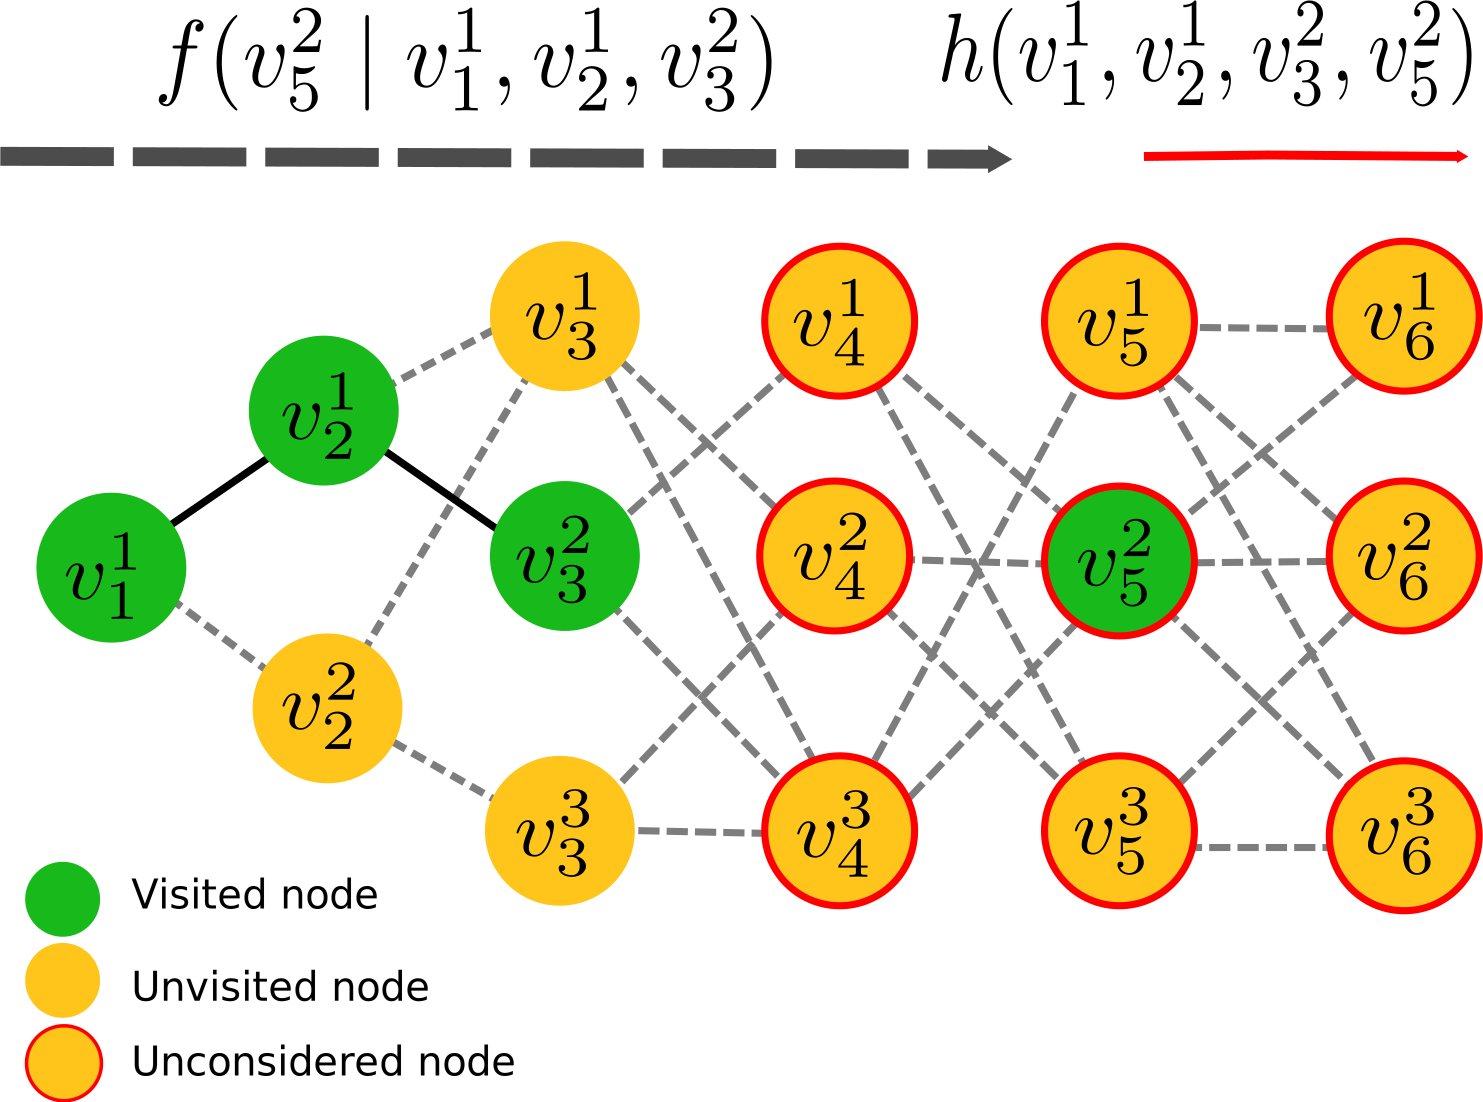
\includegraphics[width = 0.9\textwidth]{./figure/DefineFuncP}
\end{figure}
\end{block}
\end{columns}

\begin{figure}
\centering

\includegraphics[width = 0.9\textwidth]{./figure/DefineFuncHelp}
\end{figure}

\end{frame}

\begin{frame}{Backtracking}{Heuristic}

\begin{columns}

\column{0.6\textwidth}
\begin{minipage}{\textwidth}
\begin{figure}
\centering
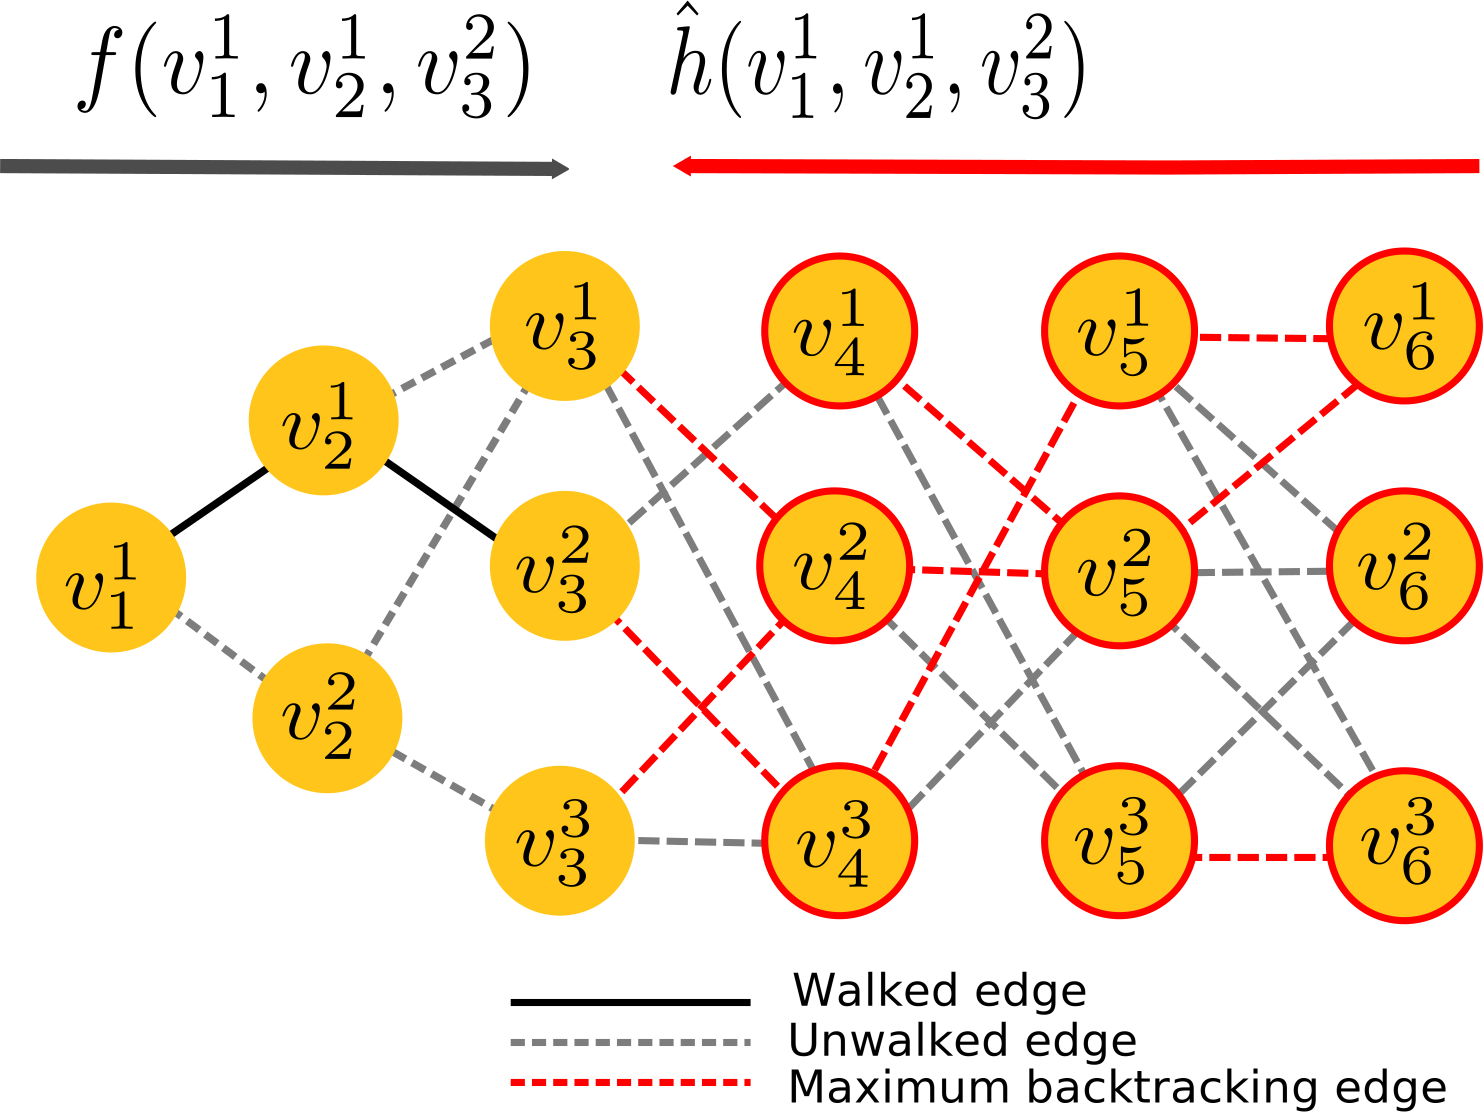
\includegraphics[width = \textwidth]{./figure/backtracking}
\end{figure}
\end{minipage}

\column{0.4\textwidth}
\begin{minipage}{\textwidth}
\begin{itemize}
\item point model $ \rightarrow $ true max total reward
\item coverage model $ \rightarrow $ estimated max total reward guarantee
\end{itemize}
\end{minipage}

\end{columns}

\end{frame}

\subsection{Anytime algorithm design}

\begin{frame}{Expanding tree}{Anytime algorithm framework}

\begin{columns}

\column{0.6\textwidth}
\begin{minipage}{\textwidth}
\begin{figure}
\centering
\includegraphics[width=.9\textwidth]{./figure/multipartite_expandingtree}
\end{figure}
\end{minipage}

\column{0.4\textwidth}
\begin{minipage}{\textwidth}
\begin{itemize}
\item depth-first recursive traverse
\item node $ \Longleftrightarrow $ subpath
\item tracking the search process
\item estimation storage
\end{itemize}
%Exapnding tree $ G_{T} = (N, L, T) $ \\
%\begin{itemize}
%\item $ T $ - tree depth
%\item $ N $ - Node set
%\item $ L $ - directed link set
%\end{itemize}
\end{minipage}

\end{columns}

\end{frame}

\begin{frame}{Node freeze}{Anytime algorithm framework}

Estimated reward $ \leq $ Current best reward 
$ \Longrightarrow $ Stop exploring subpath

\begin{figure}
\centering
\includegraphics[width =  0.8\textwidth]{./figure/freeze_process}
\end{figure}

\end{frame}

\begin{frame}{Flow}{Anytime algorithm framework}

\begin{figure}
\centering
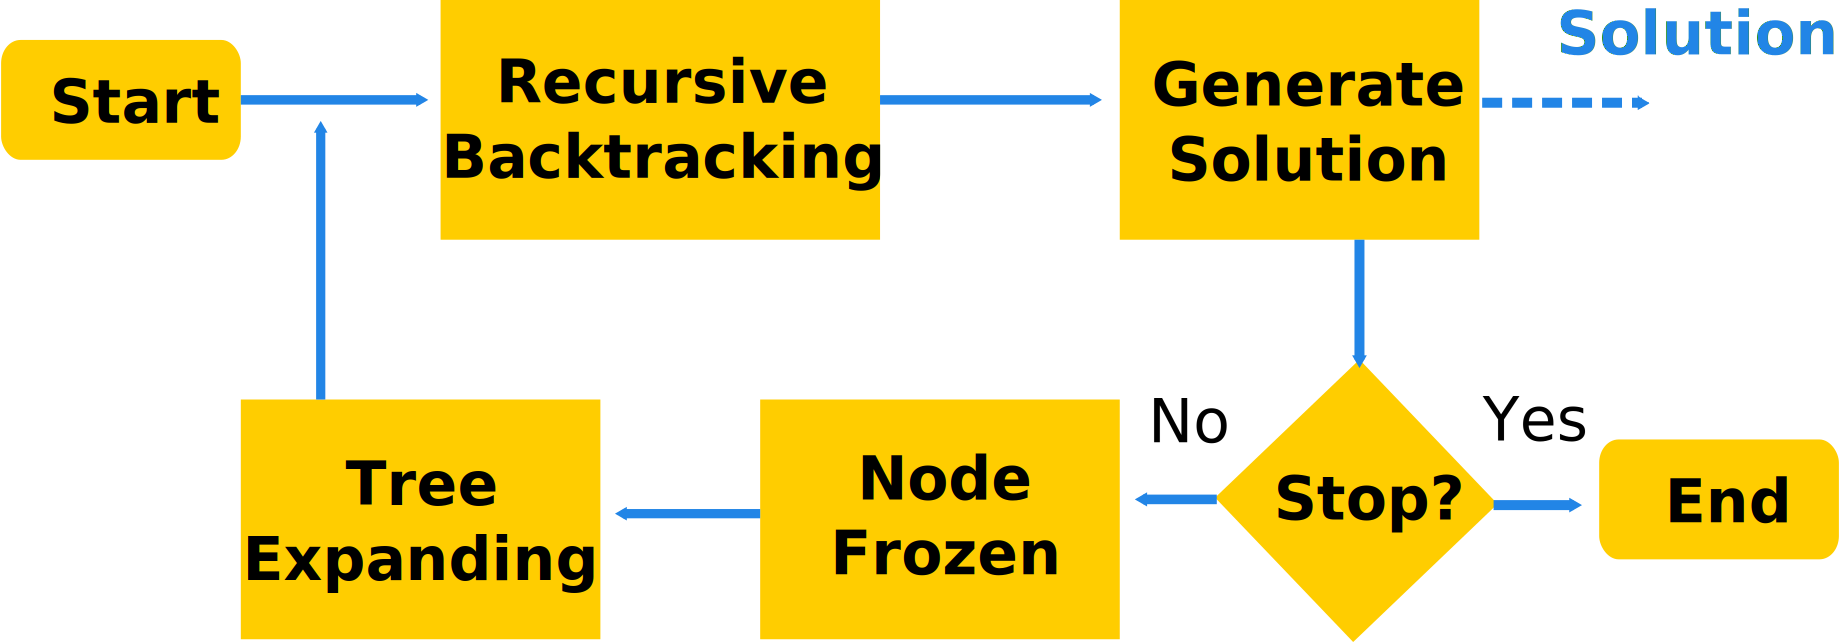
\includegraphics[width = 0.9\textwidth]{./figure/alg_flow}
\end{figure}

\end{frame}

\begin{frame}{Performance guarantee}{Anytime algorithm framework}

\begin{lemma}
“Backtracking” in Algorithm 1 never \textcolor{red}{underestimates}
the maximum total reward, which means
\begin{equation}
\nonumber
\forall t \geq t', \hat{u}(x_{t} \mid v_{1} , \cdots , v_{t'}) \geq u(x_{t} \mid v_{1} , \cdots , v_{t'}).
\end{equation}
\end{lemma}

\begin{minipage}{\textwidth}
\begin{figure}
\centering

\includegraphics[width = 0.15\textwidth]{./figure/arrow}
\end{figure}
\end{minipage}

\begin{theorem}
The anytime algorithm framework in Algorithm 4 can always find an \textcolor{red}{optimal} solution given enough time.
\end{theorem}

\end{frame}

\documentclass[conference]{IEEEtran}

\usepackage{natbib}
\usepackage{graphicx}
\usepackage{amsmath}
\usepackage{amssymb}
\usepackage{amsthm}

\newtheorem{lem}{Lemma}
\newtheorem{Hyp}{Assumption}
\newtheorem{propty}{Property}
\newtheorem{thm}{Theorem}
\newtheorem{mydef}{Definition}

\usepackage{algorithm}
\usepackage{algorithmic}
\renewcommand{\algorithmicrequire}{\textbf{Input:}}
\renewcommand{\algorithmicensure}{\textbf{Output:}}

\usepackage{subfigure}
\usepackage{float}

\begin{document}

\title{Informative Path Planning for a Wingman Robot in a Collaborative Search Task}

\author{
\IEEEauthorblockN{Daqign Yi, Michael A. Goodrich and Kevin D. Seppi}
\IEEEauthorblockA{Department of Computer Science\\
Brigham Young University\\
Provo, Utah 30332--0250\\
Email: daqing.yi@byu.edu}
}

\maketitle

\begin{abstract}
We introduce a role of a robot wingman for a search task of a human-robot team.
The path planning problem for a robot wingman is converted into a submodular orienteering problem on a multi-partite graph.
We propose a backtracking process to generate the path-search heuristic.
An expanding tree is imported to track the path search process in an anytime algorithm. 
We use a node-frozen procedure on the expanding tree to increase the search efficiency and prove that it preserves optimality.
At the end, a set of simulation results are given to illustrate the algorithm's performance and analyze the sensitivities on different parameters.
\end{abstract}

\IEEEpeerreviewmaketitle

\section{Introduction}
\label{sec:introduction}

\subsection{Human-Robot Search}
\label{subsec:cordon_and_search}

A search task focuses on walking through the search space to find target objects or persons of interest.
It has been included in many assignments, like military cordon and search \cite{waggener2010air}, wilderness search and rescue, and etc.  
The agents in a search team are usually required to collaborate to enhance the search efficiency.
The collaboration in a team search task involves information gathering and sharing in team wide of a multi-agent system.
Due to the capacity asymmetry between a robot agent and a human agent, adding a robot to a search team facilitate the team capability. 
The advantages of involving robots in a search team potentially include follows:
\begin{enumerate}
\item robots can be assigned some tasks to reduce potential danger to humans;
\item robots can deliver constant and stable performance without fatigue; 
\item robots can be equipped with a variety of sensors that can extend the perception capability of the entire team.
\end{enumerate}

\subsection{Robot Wingman}
\label{subsec:robot_wingman}

To support the collaboration in the search task, \cite{goodrich2013toward} introduce a robot wingman. 
The robot wingman defines a type of human-robot relationship in a team, which is to have a robot that accompanies a human when the human navigates through some space.
Besides the advantages from a robot agent in a search team, a robot wingman can also
\begin{enumerate}
\item detect threats or opportunities that may be relevant to the human but likely not seen by the human;
\item be responsive to an assistance request from a human agent in the team. 
\end{enumerate}

\begin{figure}[htbp]
\centering
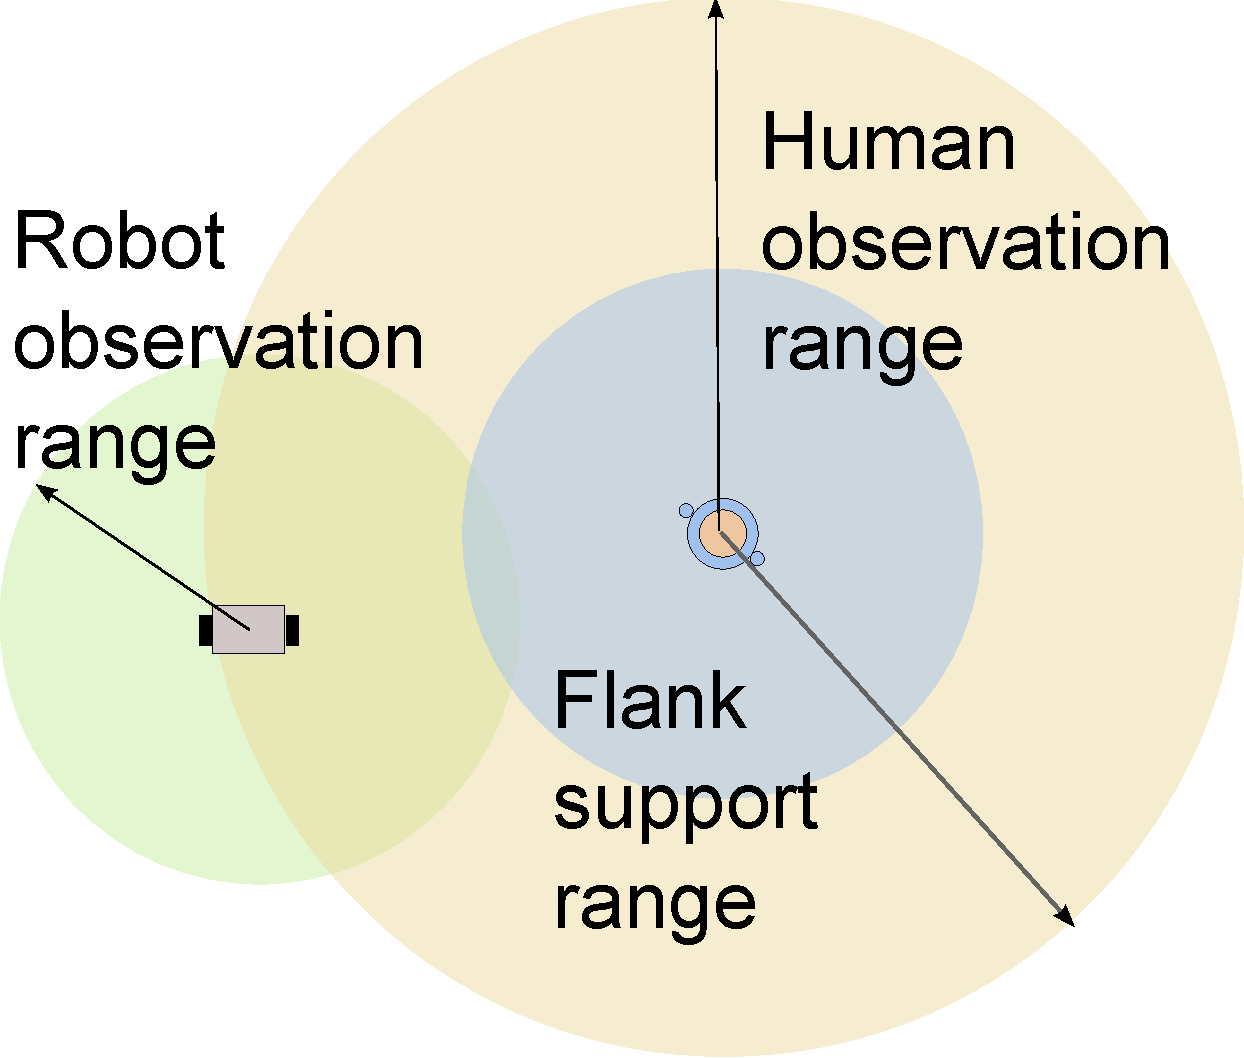
\includegraphics[width=0.4\textwidth]{./images/Wingman.pdf}
\caption{A Robot Wingman Framework.}
\label{fig:Wingman}
\end{figure}

The paper proceeds as follows.
We give a brief review on how the model is usually modeled and how the problems are solved in Section \ref{sec:related_work}.
Section \ref{sec:problem_statement} gives how the problem is modeled into an information maximization problem and how a multi-partite graph is generated using the wingman constraint.
Section \ref{sec:path_dependent_optimization} formulates the problem into a class of submodular orienteering on a multi-partite graph.
Section \ref{sec:tree_expanding_search} proposes the algorithms on solving the submodular orienteering and provides the proof on the  performance.
Section \ref{sec:simulation_and_analysis} analyzes the performance and efficiency of the proposed algorithm in different scenarios and parameters.


\section{Related Work}
\label{sec:related_work}

If we assume that search targets are static in the search environment, the scan on a location decreases the estimated probability that there is some search target here.
Observations in a search process reduce the uncertainty of where search targets locate.
By measuring this type of uncertainty with information, a search agent can collect more information at non-observed locations than observed ones.
Information gathering is usually selected to measure the efficiency of a search task.
In this paper, we focus on path planning in a search task answers how to maximize information with limited time and resource by defining objective in forms of information evaluation \cite{goodrich2013toward}.

Research work on information maximization path planning focuses a lot on how to solve the optimization problems defined in large scale solution spaces in reasonable time.
\cite{levine2010information} imports ideas of RRT to an information-rich path planning problem, which targets at bringing good efficiency in online optimization in a continuous space.
Under a temporal logic constraint, \cite{JonesSchwagerBeltaICRA13scLTLInfo} use a receding horizon planning to solve an online information-gathering optimization problem.

\begin{figure}
\centering
\includegraphics[width=0.4\linewidth]{./images/robotObservation.pdf}
\caption{Maximum coverage in robot observation.}
\label{fig:robotObservation}
\end{figure}

Usually the observation of a search agent covers a much larger region than the area occupied by the robot's body, which is shown in Figure \ref{fig:robotObservation}.
If we consider the observation as a covering range instead of a cell or a point, the overlaps between observation coverage at different time steps must be considered when measuring the total quantity of information.
Figure \ref{fig:robotObservation} gives an example.

Mutual information and conditional mutual information are commonly used to model the overlaps in measuring the total information \cite{singh2009efficient}.
This belongs to a \emph{maximum coverage problem}. 
Multiple sensors placement is one of the applications on information maximization.
In a sequential placement, the locations of placed sensors determine the increase on total information by adding a new sensor.
It is known to be a classical NP-hard combinatorial optimization problem \cite{megiddo1983maximum}.
The problem of maximum coverage on information measurement implies a property of ``nondecreasing submodularity''. 

Maximizing the score collected from a limited-length graph walk is usually known as an \emph{orienteering problem} \cite{Vansteenwegen20111}, in which the total score is a summation of the scores of visited vertices.
If the score function of a vertex has submodularity as in a \emph{maximum coverage problem}, the problem is defined as a \emph{submodular orienteering problem} \cite{chekuri2005recursive}.
A greedy approximation with known performance bound proposed in \cite{singh2009efficient} efficiently exploits the submodularity property of mutual information.
Similarly, in a branch and bound way, \cite{binney2012branch} apply greedy search to informative path planning.
Because the location of the robot at time $ t $ constrains the reachable location at time $ t+1 $, applying greedy algorithm with ``teleport'' assumption to the problem with this constraint can be extremely bad \cite{krause2012submodular}.
In non-teleport motion, \cite{chekuri2005recursive} import recursive greedy by converting to a knapsack constraint so that there is a time resource allocation on planning steps.

Due to the wingman constraint, the path planning of a robot wingman depends on a temporal-space synchronization requirement determined by the positions of a human through time.
The time allocation is fixed and depends on how the human's positions are sampled.
Thus we are not able to model time resource as budget in \cite{chekuri2005recursive}.   

We define the path planning of the robot wingman in a search task as an information maximization problem on a topological graph. We propose an algorithm to solve it as submodular orienteering . The algorithm is designed to produce acceptable robot performance and to be computed efficiently. We then use simulation to demonstrate the acceptable performance of the algorithm and computation efficiency. 


\section{Problem Statement}
\label{sec:problem_statement}

In this section, we discuss the details of a robot wingman in a human-robot team and define a model for the wingman path planning problem in a human-robot team search task.

We consider the search problem on a discrete map.
Let $ I $ denote the set of cells in the map.
We refer to the object or person of interest as the \emph{search target}.
For the cordon and search problem, we are using an occupancy grid representation where for each cell in the discretized space we classify the cell as being either occupied by a search target.
For each cell $ i \in I $, let $ S_{i} $ denote the binary random variable that whether there is a search target in cell $ i $.
$ P(S_{i}) $ is its probability and $ H(S_{i}) $ is its entropy.

We define a flank support range $ \gamma_{flank} $ to model the robot wingman constraint. 
This range determines the area that a robot wingman is expected to stay in when a human is moving, which is shown in Figure \ref{fig:Wingman}.
Let $ x_{t} $ denote the position of the robot wingman at time $ t $ and $ y^{h}_{t} $ denote the position of the human at time $ t $.
The robot wingman constraint requires that $ \forall t, || x_{t} - y^{h}_{t} || \leq \gamma_{flank} $.
For a discretized state space, this same definition holds as long as we define the human's and the robot's positions as the center of the cell.
In a search task, we assume that both human and robot can observe a circular area around themselves, which is defined in the same way as the flank support range as shown in Figure \ref{fig:Wingman}.
The observation ranges are $ \gamma^{human}_{obsRange} $ and $ \gamma^{robot}_{obsRange} $.
This means that an agent can observe not only the visited cell but neighboring cells in a range.
We use a neighbor function $ N^{a}_{r}(\cdot) $ to denote a set of cells satisfying some constraints of a given node, in which $ a $ denotes the application usage and $ r $ gives the range parameter.
$ N^{flank}(\cdot) $ defines the allowable cells for the robot's location given the human's position, $ N^{human}_{obsRange}(\cdot) $ and $ N^{robot}_{obsRange}(\cdot) $ define the observable cells given a position of a human and a robot, respectively.

The discrete map can be used to form the topology defining the connections between accessible positions.
Figure \ref{fig:LayerStructure} illustrates how the topological graph is formed from a real world map.
In this paper, we consider path planning on a topological graph, in which there is dependence on a human path.

\begin{figure}[htbp]
\centering
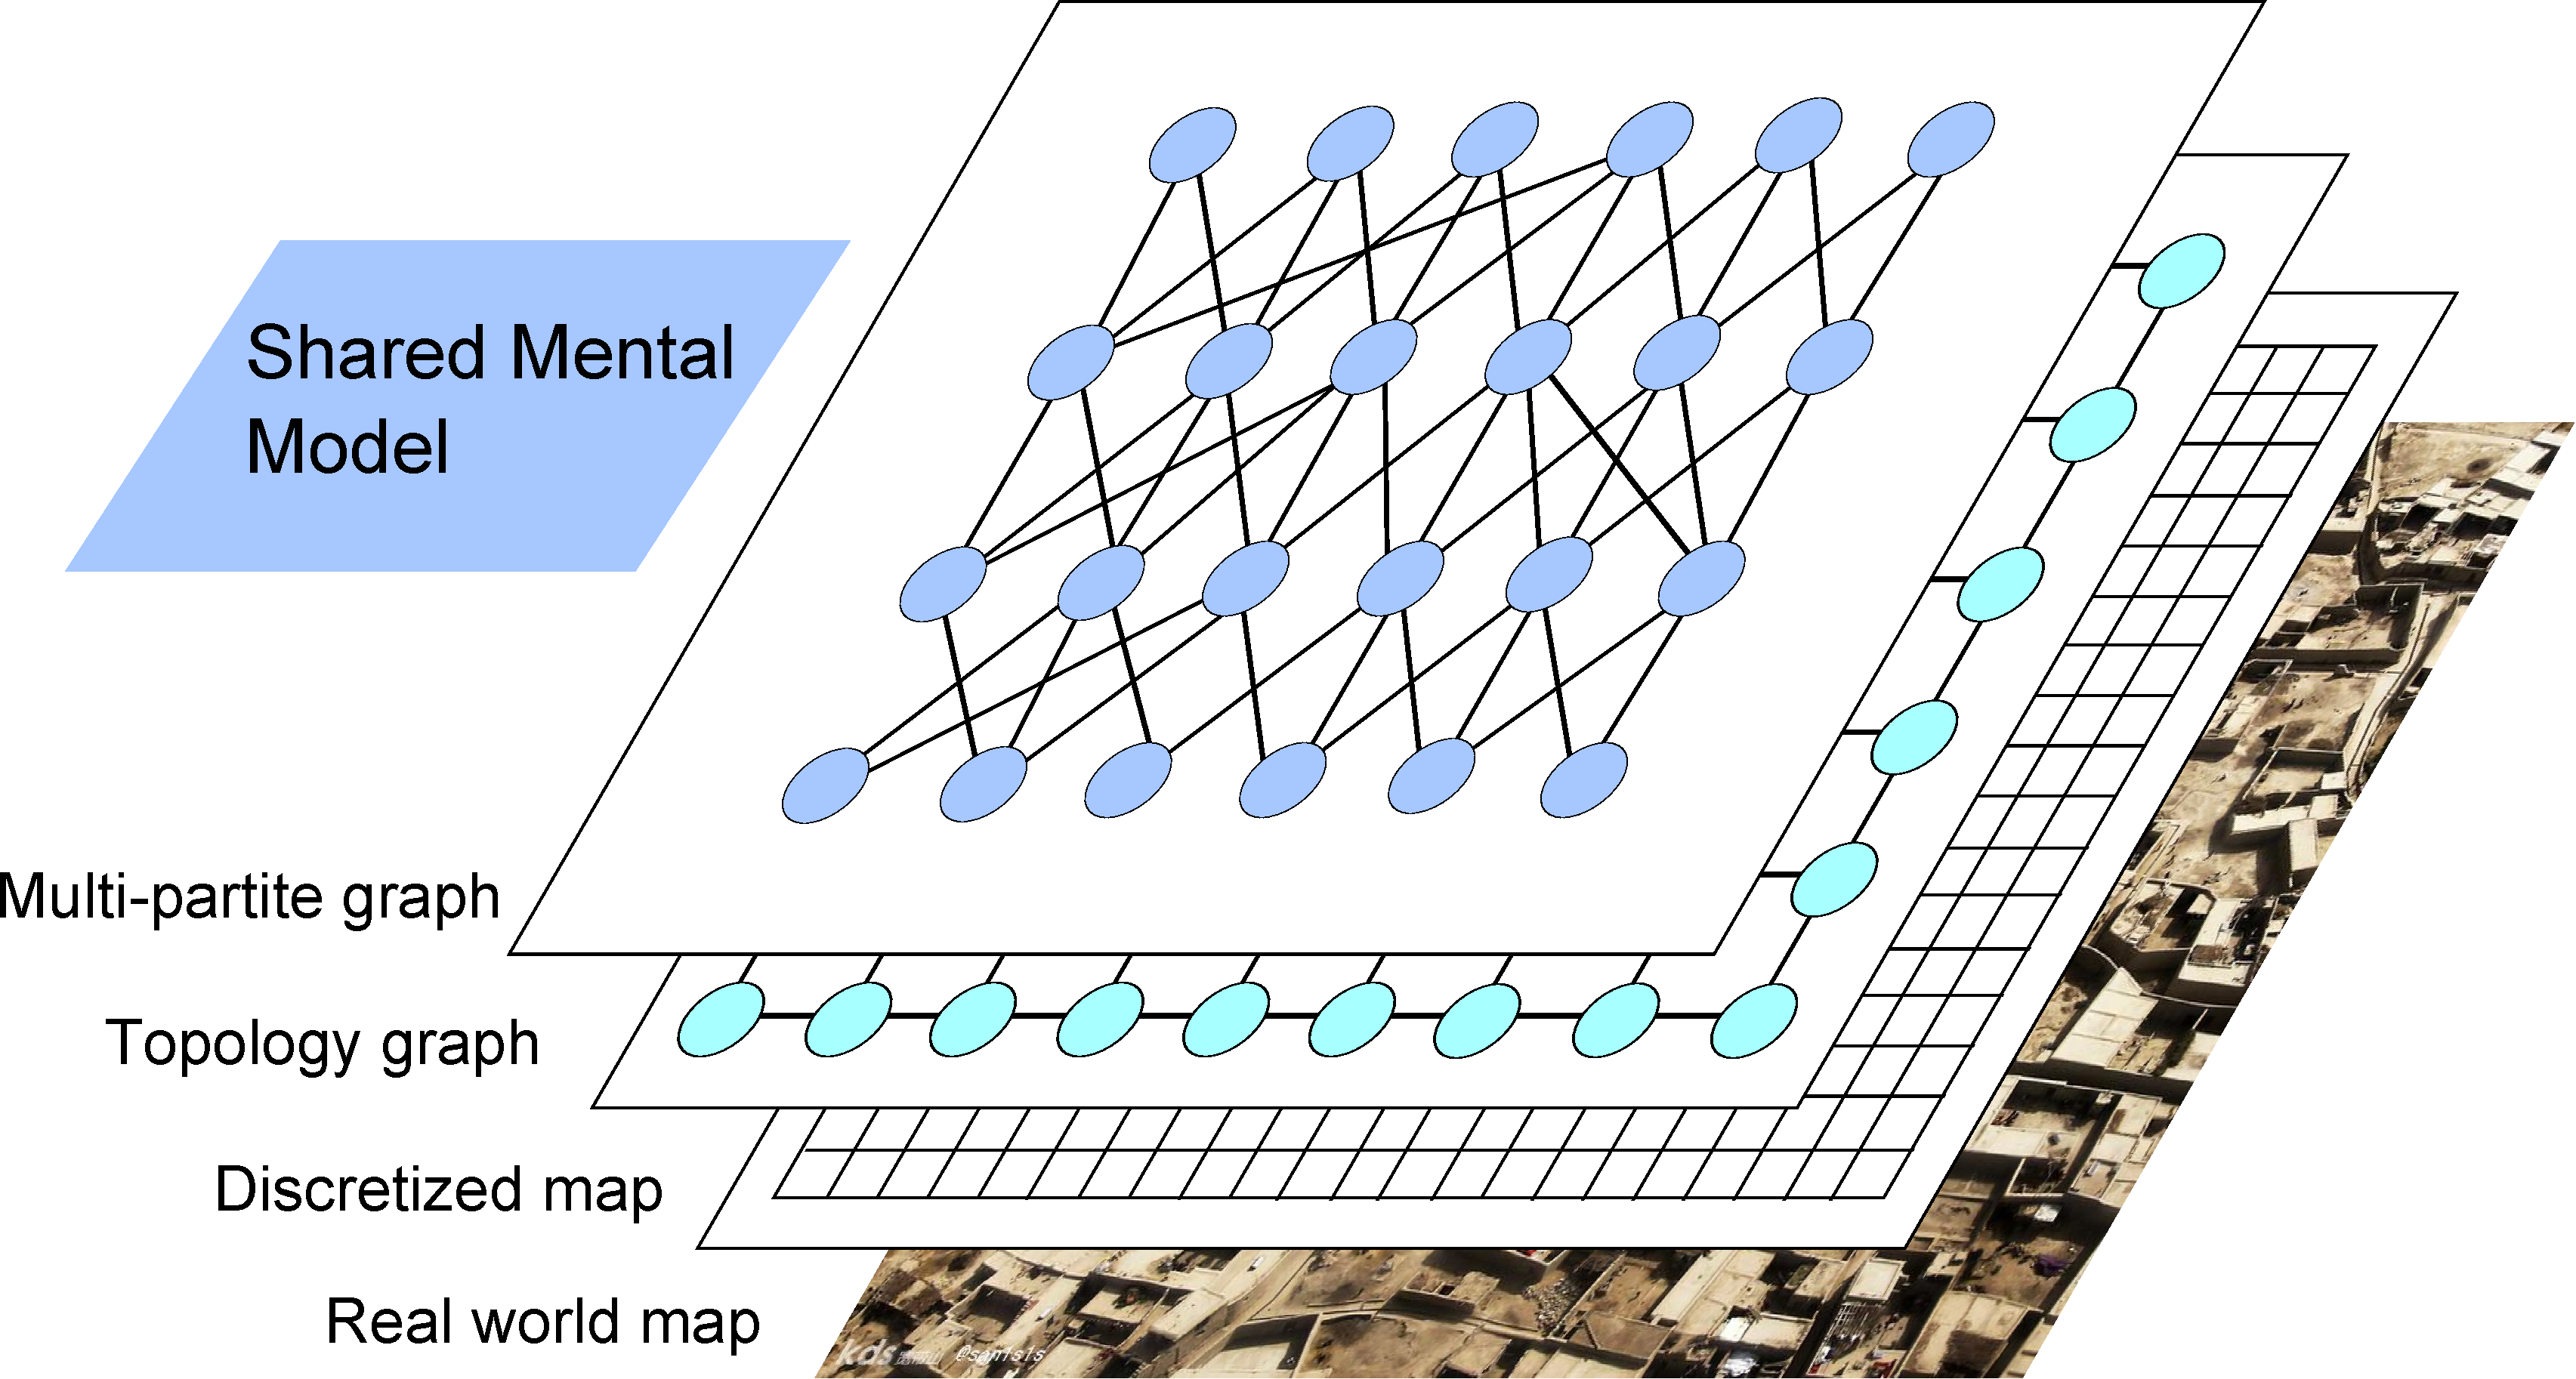
\includegraphics[width=0.45\textwidth]{./images/LayerStructure.pdf}
\caption{A layer structure of problem abstraction from real world of search space to topological description.}
\label{fig:LayerStructure}
\end{figure}

\subsection{Human Path Dependence}
\label{subsec:human_path_dependence}
 
A path of an agent is expressed as a sequence of vertices in a topology. 
In a time length of $ T $, let a vector $ Y^{h} = [y^{h}_{1}, y^{h}_{2} , \cdots , y^{h}_{T}] $ define a path of the human.
Similarly, we have a path of the robot as $ X = [x_{1}, x_{2} , \cdots , x_{T}] $.
Note that this assumes that the robot's speed matches the human's speed.
$ N^{human}_{obsRange}( y^{h}_{t} ) $ determines a set of observations made by the human at location $ y^{h}_{t} $, which is denoted as  $ O^{Y^{h}}_{t} $.
Let $ \mathbf{O}^{Y^{h}} = \{ O^{Y^{h}}_{1}, \cdots , O^{Y^{h}}_{T-1}, O^{Y^{h}}_{T} \} $ denote the sequence of these sets.
Define $ \mathbf{O}^{X} $ similarly.

We adopt Bayes rule to update the probability estimation through observations, which results in entropy reduction.
By considering the entropy reduction as information gathered by the robot, our goal is to maximize the information gained by moving the robot in the world.
In this paper, we focus on an offline path planning problem under four assumptions \ref{Assumption1} , \ref{Assumption2} , \ref{Assumption3} and \ref{Assumption4}.

\begin{Hyp}
\label{Assumption1}
The human path is known.
\end{Hyp}

\begin{Hyp}
\label{Assumption2}
There is a human observation model, which can be used to predict what the human will and will not see in the world.
\end{Hyp}

\begin{Hyp}
\label{Assumption3}
The search environment is time-invariant.
\end{Hyp}

\begin{Hyp}
\label{Assumption4}
The observation models of both the human and the robot are time-invariant and spatially independent.
\end{Hyp}

Assumptions \ref{Assumption1} and \ref{Assumption2} allow us to determine the distribution of $ \mathbf{O}^{Y^{h}} $, which is applied to update the estimated probability on where the search target is before doing path planning of the robot.
By Assumptions \ref{Assumption3} and \ref{Assumption4}, we can derive Property \ref{prop:orderIndependence}.

\begin{propty}
\label{prop:orderIndependence}
Given a path $ X = [ x_{1}, x_{2} , \cdots , x_{t} ]^{T} $, the total information can be collected is independent with the visiting sequence.
\begin{proof}
See the proof in Appendix \ref{app:order_independence}
\end{proof}
\end{propty}


We use conditional mutual information to evaluate the information gain of the robot.
In equation \eqref{eq:condMutInf}, this means that the entropy reduction on uncertainty estimation on the search space $ \mathbf{S} $ due to the observation of a robot $ \mathbf{O}^{X} $ when the observation of a human $ \mathbf{O}^{Y^{h}} $ is given.

\begin{equation}
\label{eq:condMutInf}
\begin{aligned}
I(\mathbf{S}; \mathbf{O}^{X} \mid \mathbf{O}^{Y^{h}}) & = H(\mathbf{S} \mid \mathbf{O}^{Y^{h}}) - H(\mathbf{S} \mid \mathbf{O}^{X},\mathbf{O}^{Y^{h}})\\
& = H(\mathbf{O}^{X} \mid \mathbf{O}^{Y^{h}}) - H(\mathbf{O}^{X} \mid \mathbf{O}^{Y^{h}}, \mathbf{S}).
\end{aligned}
\end{equation}

The information maximization of a robot in a search problem can be defined as an optimization problem, which is:

\begin{equation}
\label{eq:objFunc}
\begin{aligned}
Objective: X^{*} = \underset{X}{\arg\max} [I(\mathbf{S}; \mathbf{O}^{X} \mid \mathbf{O}^{Y^{h}})] \\
Constraint: \forall t, x^{t} \in N^{flank}(y_{t}) \cap N^{robot}_{1}(x^{t-1}) 
\end{aligned}
\end{equation}

Due to the existence of the potential overlap between robot observation regions of different times, the entropy reduction by $ O^{X}_{t} $ depends on $ O^{X}_{1} , \cdots , O^{X}_{t-1} $ as well.
This is stated in Lemma \ref{Lemma1}.

\begin{lem} 
\label{Lemma1}
When the human observation $ \mathbf{O}^{Y} $ is known, we can factor the objective in equation \eqref{eq:condMutInf} into a chain rule form,
\begin{equation}
\label{eq:offHmPathChain}
\begin{aligned}
I(\mathbf{S}; \mathbf{O}^{X} \mid \mathbf{O}^{Y^{h}}) & = \sum_{t=1}^{T} H(O_{t}^{X} \mid O_{1}^{X} , \cdots , O_{t-1}^{X}, \mathbf{O}^{Y^{h}}) - \sum_{t=1}^{T} H(O_{t}^{X} \mid O_{1}^{X} , \cdots , O_{t-1}^{X}, \mathbf{S}, \mathbf{O}^{Y^{h}}) \\
& = \sum_{t=1}^{T} I(O^{X}_{t} ; \mathbf{S} \mid O^{X}_{1} , \cdots , O^{X}_{t-1}, \mathbf{O}^{Y^{h}})
\end{aligned}
\end{equation}
\begin{proof}
The proof follows trivially from the definition of conditional probability and conditional mutual information. 
The detail is given in Appendix.
\end{proof}
\end{lem}

In equation \eqref{eq:offHmPathChain}, we can express the maximum total information as a summation of maximizing information at each step, which indicates a sequential substructure in solving the maximization problem.
Thus we look into the solution space and the optimization at each single planning step.

\subsection{Unfold Solution Space of Single Step Through Time}
\label{subsec:unfold_solution_space}

%We find that there exists a temporal-space relationship between a robot wingman and a human.
%a solution space at one time step for a robot is a set of positions defined by $ N^{flank}() $ and a human position $ y^{h}_{t} $.
When assumption \ref{Assumption1} stands, the solution space of a robot wingman at a single time step is determined by $ N^{flank}() $ and a human position $ y^{h}_{t} $. Unfolding the solution spaces at different time steps generates a multi-partite graph for path planning. Figure \ref{fig:MultiPartite} gives an example. A partition of time $ t $ indicates a set of vertices which are allowed for the robot wingman to visit at time $ t $. As expressed in Figure  \ref{fig:LayerStructure}, the topological graph determines the edges between vertices in the multi-partite graph.

\begin{mydef}[\textbf{Multi-Partite Graph}]
\label{def:multi_partite}
The multi-partite graph $ G = (V, E, T) $ is defined as
\begin{itemize}
\item The number of partitions is $ T $.
\item The vertex set $ V $ is defined as $ V = \cup_{t=1}^{T} V(t) $.
Each partition $ V(t) $ is a set of vertices $ v^{i}_{t} $, where $ t $ indicates which partition the vertex $ x $ is in and $ i $ indicates the index of this vertex.
\item Edges are directed, originating from vertices in set $ V(t) $ to vertices in set $ V(t+1) $.
Let $ v^{i}_{t} \in V(t) $ and $ v^{j}_{t+1} \in V(t+1) $.
A directed edge $ (v^{i}_{t}, v^{j}_{t+1}) $ connects vertices $ v^{i}_{t} $ and $ v^{j}_{t+1} $. 
\end{itemize}
\end{mydef}

Figure \ref{fig:MultiPartite} gives an example on a multi-partite graph converted from a topological graph.
Each partition $ V(t) $ is determined by $ V(t) = N^{flank} ( y^{h}_{t} ) $.
There is a directed edge that connects vertices $ v^{i}_{t} $ and $ v^{j}_{t+1} $ only if there is an edge that connects them in the topological graph.

\begin{figure}[htbp]
\centering
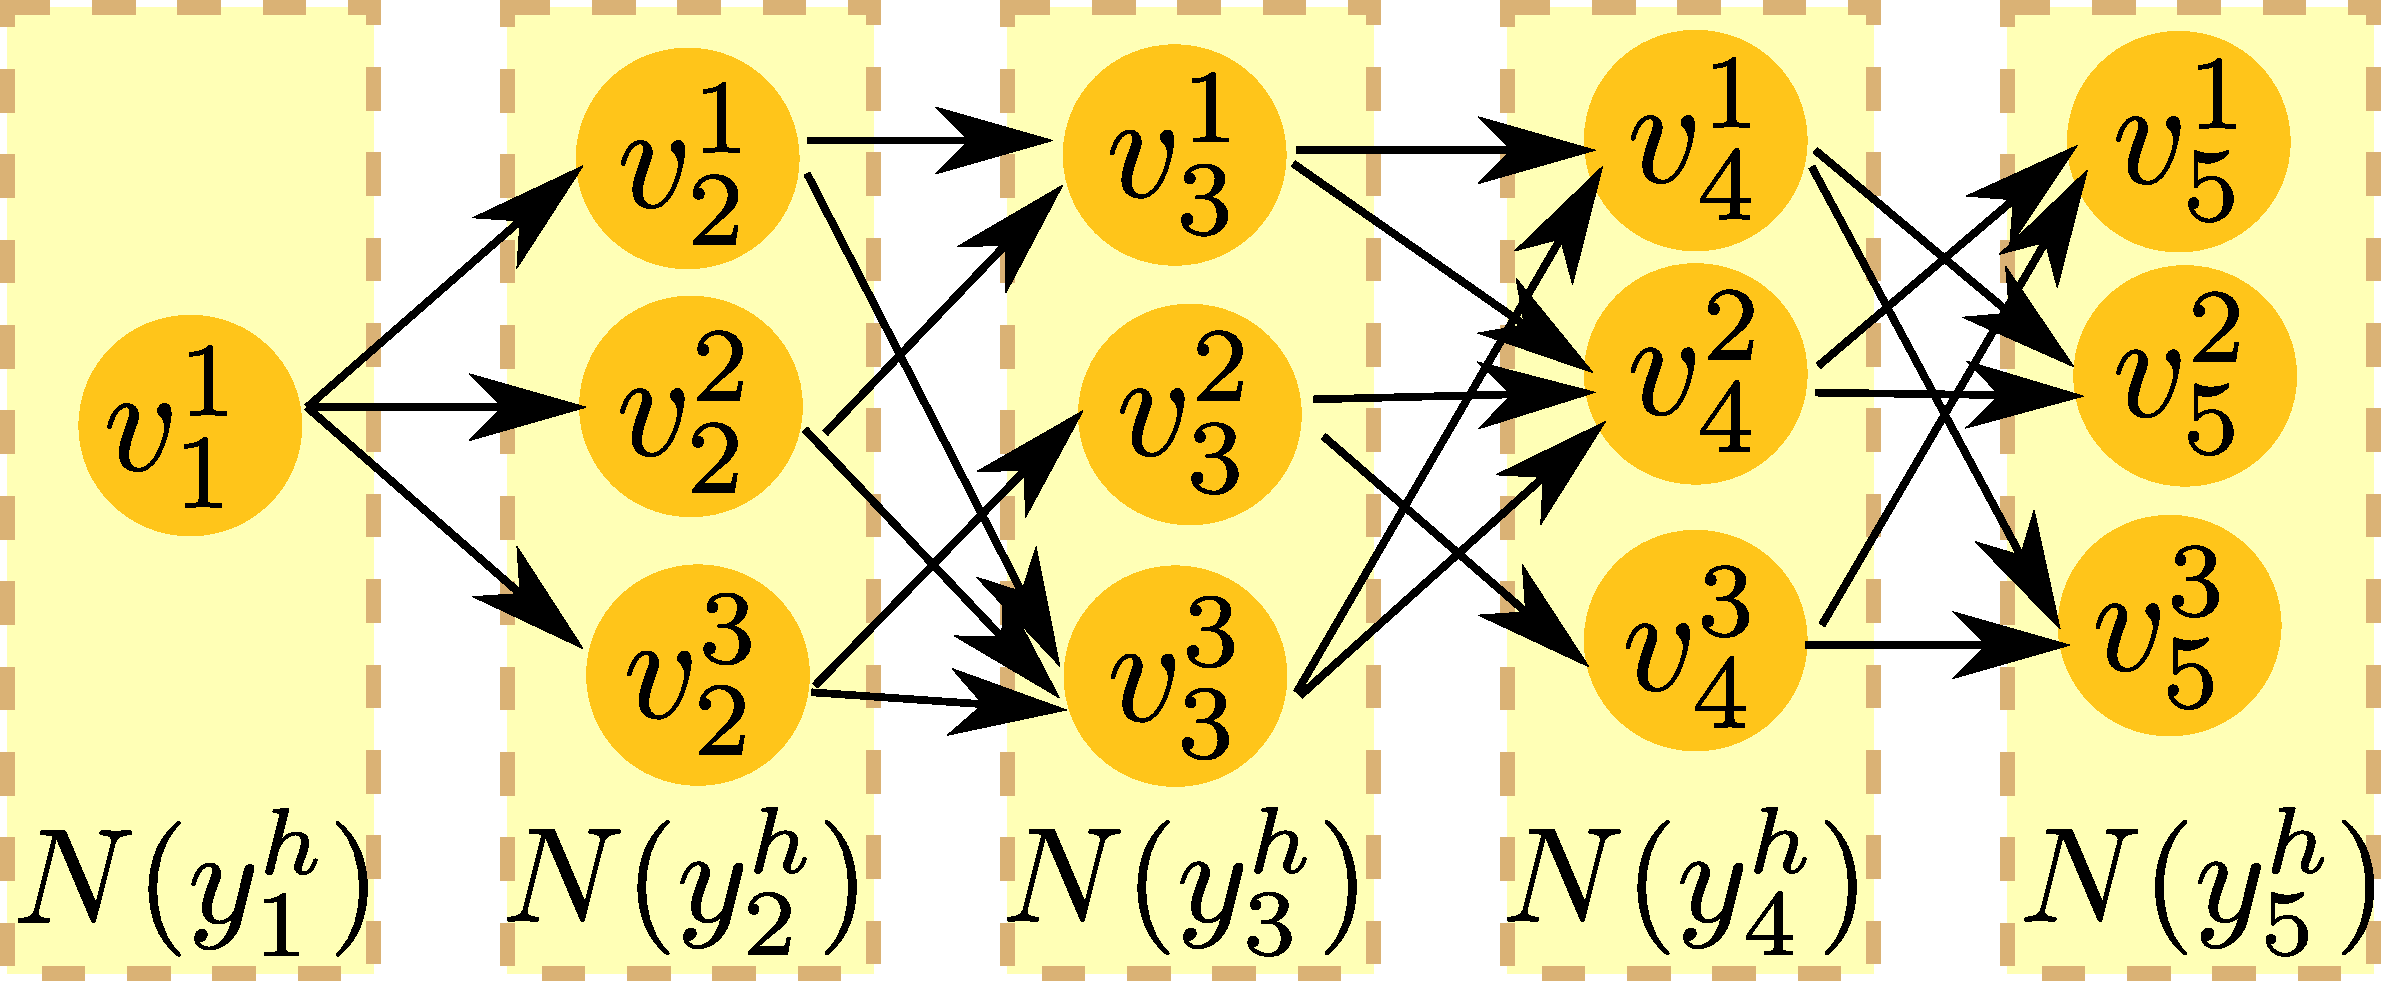
\includegraphics[width=0.4\textwidth]{./images/MultiPartite.pdf}
\caption{A multi-partite graph for robot wingman search.}
\label{fig:MultiPartite}
\end{figure}
 
If a vertex $ v^{i}_{t} $ cannot be reached from any vertex in partition $ V(t-1) $ or does not go into any vertex in partition $ V(t+1) $, it will never be in a path of length $ T $.
Here we use a pruning process to remove those ``useless'' vertices in a planning problem.
The pruning process consists of forward pruning and backward pruning.
The forward pruning starts from partition $ V(2) $ to partition $ V(T) $.
Any vertex that has no in edge and its incident edges will be removed.
The backward pruning starts from partition $ V(T-1) $ to partition $ V(1) $.
Any vertex that has no out edge and its incident edges will be removed.
\footnote{In forward pruning, removing a vertex and its incident edges in $ V(t) $ might only make vertices in $ V(t+1) $ having no in edge.
Those vertices will be removed when pruning in $ V(t+1) $.
Similarly, in backward pruning, removing a vertex and its incident edges in $ V(t) $ might only make vertices in $ V(t-1) $ having no out edge.
Those vertices will be removed when pruning in $ V(t-1) $.  
This means that two prunings will not make any vertex has no in edge or has no out edge.
Thus, the properties of ``non-terminating'' and ``reachable'' can be guaranteed.}
After the pruning, the multi-partite graph has below two properties.
\begin{itemize}
\item \emph{Non-terminating:} From $ V(1) $ to $ V(T-1) $, any vertex has an out edge to a vertex in the next partition, which ensures that $ \forall t \in \{ 1 , \cdots , T-1 \} \forall v^{i}_{ t } \in V( t )  ( deg^{+}(v^{i}_{ t }) > 0 )  $.
\item \emph{Reachable:} From $ V(T) $ to $ V(2) $, any vertex has an in edge from a vertex in the previous partition, which ensures that $ \forall t \in \{ 2, \cdots , T \} \forall v^{i}_{ t } \in V( t )  ( deg^{-}(v^{i}_{ t }) > 0 )  $. 
\end{itemize}

\section{Submodular Orienteering on a Multi-Partite Graph}
\label{sec:path_dependent_optimization}

Using the wingman constraint, we have converted the path-planning problem on a topological graph to a path-planning problem on a multi-partite graph.
Using the observation model and the information measurement we defined, the reward collection can be described by a submodular function $ f() $ [\cite{goodrich2013toward}].
In this section, we will merge these two properties to define a submodular orienteering problem on a multi-partite graph.


\begin{mydef}[\textbf{Submodular Function}][\cite{krause2012submodular}]
\label{def:submod_func}
A submodular function over a set $ V $ is a function  $ f : 2^{V} \rightarrow \mathbb{R} $ that satisfies for every $ A, B \subseteq V $,
\begin{equation}
\label{eq:submod}
f(A \cap B) + f(A \cup B) \leq f(A) + f(B).
\end{equation}
\end{mydef}

A \emph{conditional submodular function} can be similarly defined.

\begin{mydef}[\textbf{Conditional Submodular Function}]
\label{def:cond_submod_func}
A conditional submodular function over a set $ V $ is a function $ f : 2^{V} \times 2^{V} \rightarrow \mathbb{R} $, which is defined for all $ A, B \subseteq V $, 
\begin{equation}
\label{eq:cond_submod}
f( A \mid B ) = f( A \cap B ) - f( B ).
\end{equation}
This function inherits the submodularity, which means that every $ A, B, C \subseteq V $,
\begin{equation}
\label{eq:cond_submod_prop}
f(A \mid B \cup C) \leq f(A \mid B).
\end{equation}

See the proof in Appendix \ref{app:cond_submod_prop}.

\end{mydef}

Without loss of generality, we write $ f( x_{1} , \cdots x_{t} ), x_{1} , \cdots x_{t} \in X $ to indicate that $ f( \{ x_{1} , \cdots x_{t} \}) $.
This notational convenience will also be used for the \emph{conditional submodular function} in equation \eqref{eq:cond_submod}.

%By Lemma \ref{Lemma1}, we have the human's path $ Y^{H} $ known.
%Thus the wingman constraint can be converted into a multi-partite graph like Figure \ref{fig:MultiPartite} in Section \ref{sec:unfold_solution_space}.
By Lemma \ref{Lemma1}, we know that the optimal solution at one time step depends on the solutions chosen at previous time steps. 
In [\cite{krause2012submodular}], it was shown that the entropy and mutual information functions are both submodular.
Thus, the path-dependent optimization problem can be formally defined as a \emph{submodular orienteering on a multi-partite graph}, as follow:

\begin{mydef}[\textbf{Submodular Orienteering on a Multi-Partite Graph}]
\label{def:submod_orienteer}
Given a directed multi-partite graph $ G = (V, E, T) $, each edge $ e \in E $ defines a directed transition from a vertex in partition $ V(t) $ to a vertex in partition $ V(t+1) $, $ t \in [1, T-1] $.
The submodular orienteering problem on a directed multi-partite graph $ G $ is to find a path of length $ T $ that maximizes the total reward collected from a submodular function $ f() $.
\end{mydef}

Without loss of generality, we assume that the optimal search for path planning always starts from same vertex.
Thus, we have only one vertex in partition $ V(1) $, which is shown in Figure \ref{fig:MultiPartite}.
By the submodularity of the conditional mutual information, we can represent $ I(\mathbf{S}; \mathbf{O}^{X} \mid \mathbf{O}^{Y^{h}}) $ by a submodular function  $ f(X) $. 
By Definition \ref{def:submod_orienteer}, we can rewrite equation 
 \eqref{eq:objFunc} as 

\begin{equation}
\label{eq:gnr_obj}
\begin{aligned}
Objective: & X^{*} = \underset{X}{\arg\max} f(X); \\
Constraint: & |X| = T, x_{t} \in V(t), (x_{t}, x_{t+1}) \in E.
\end{aligned}
\end{equation}

Due to Property \ref{prop:orderIndependence}, we write $ f( [x_{1}, x_{2} , \cdots , x_{t} ]^{T} ) $ as $ f(x_{1}, x_{2}, \cdots , x_{t}) $ for simplicity.

By Definition \ref{def:submod_func}, Definition \ref{def:cond_submod_func} and Lemma \ref{Lemma1}, we have
\begin{equation}
\label{eq:gnr_f_chain}
f(x_{1}, x_{2}, \cdots , x_{T}) = f(x_{1}) + f(x_{2} \mid x_{1}) + \cdots + f(x_{T} \mid x_{1}, \cdots , x_{T-1}).
\end{equation}

If we let $ \hat{x}_{t} $ denote the answer to the optimality found at time step $ t $ in considering payoff to arrive and payoff to go,  we can have optimal substructures solved as 
\begin{equation}
\label{eq:max_2}
\hat{x}_{t} = \arg \max_{X_{t}} \left[ f(x_{t} \mid x_{1} , \cdots , x_{t-1})
+ \max_{X_{t+1}, \cdots , X_{T}} f(x_{t+1}, \cdots , x_{T} \mid x_{1}, \cdots , x_{t})
\right].
\end{equation}

$ X_{t} $ is defined by the constraint in equation \eqref{eq:objFunc}, which indicates the search space at time step $ t $.
In order to solve equation \eqref{eq:max_2}, we define the first term as \emph{instant reward} and the second term as \emph{maximum future reward}.

\begin{mydef}[\textbf{Instant Reward}]
\label{def:instant_reward}
Define the instant reward as 
\begin{equation}
\label{eq:def_g}
g(x_{t} \mid x_{1} , \cdots , x_{t-1} ) = f(x_{t} \mid x_{1} , \cdots , x_{t-1}). 
\end{equation}
\end{mydef}

By definition \ref{def:cond_submod_func}, instant reward represents the reward collected by choosing $ x_{t} $ after $ x_{t-1} , \cdots , x_{1} $ have been visited.

\begin{mydef}[\textbf{Maximum Future Reward}]
\label{def:max_future_reward}
Define the maximum future reward as
\begin{equation}
\label{eq:def_h}
h(x_{1} , \cdots, x_{t'} ) = \max_{V(t'+1), \cdots , V(T)} f(x_{t+1}, \cdots x_{T} \mid x_{1}, \cdots , x_{t'}),
\end{equation} 
in the constraint that
\begin{equation}
\label{eq:def_h:constraint1}
\forall \tau \in \{ t'+1 , \cdots , T \},  x_{\tau} \in V(\tau)
\end{equation}
and
\begin{equation}
\label{eq:def_h:constraint2}
\forall \tau \in \{ t'+2, \cdots ,T-1 \}, ( x_{\tau-1}, x_{\tau} ) \in E .
\end{equation}
\end{mydef}

\begin{figure}
\centering
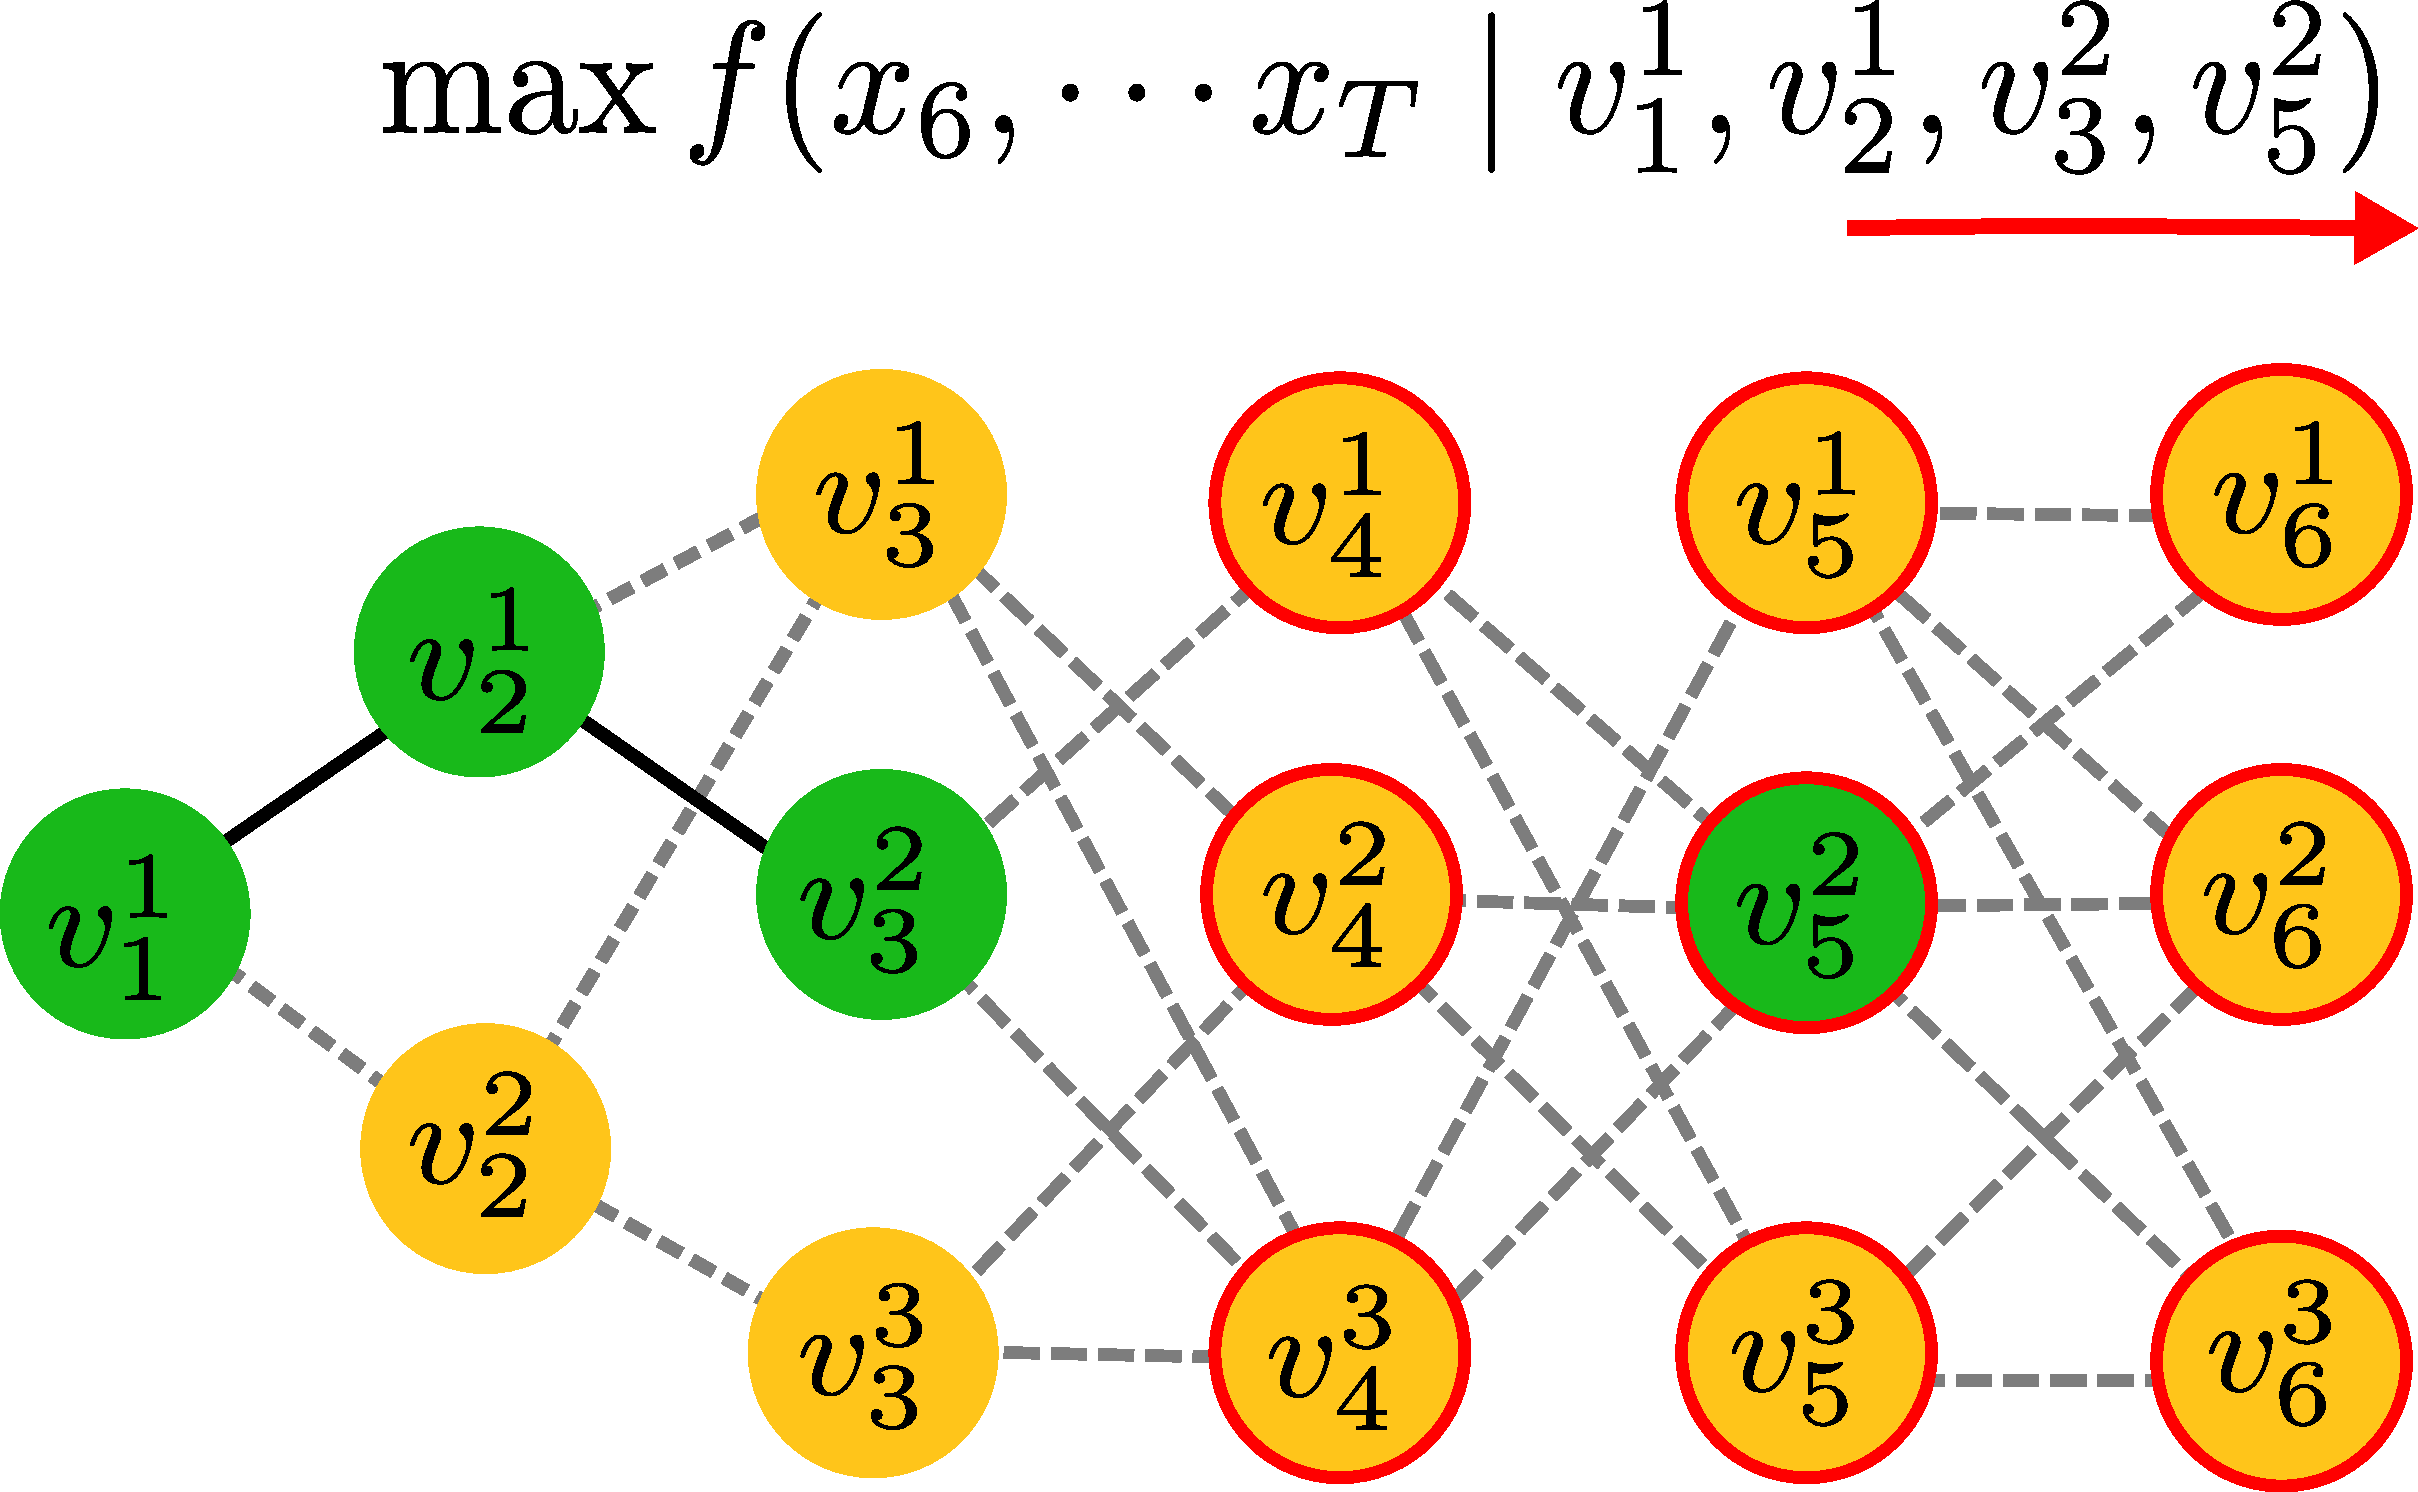
\includegraphics[width=0.5\linewidth]{./images/DefineFuncH.pdf}
\caption{Maximum future reward.}
\label{fig:DefineFuncH}
\end{figure}

The function $ h() $ indicates the maximum future reward of a sub-path that concatenates $ x_{t} $ after $ \{  x_{1} , \cdots, x_{t} \} $ has been visited. 
$  x_{t} $ has the biggest time index in $ \{  x_{1} , \cdots, x_{t-1} , x_{t} \} $.
We would like to figure that in defining the instant reward and the maximum future reward, $ \{  x_{1} , \cdots, x_{t-1} , x_{t} \} $ can be any set of vertices instead of a set of vertices in a sub-path.

Figure \ref{fig:DefineFuncH} gives an example on how $ h(v^{1}_{1}, v^{1}_{2}, v^{2}_{3}, v^{2}_{5}) $ is calculated.
There exists a jump from partition $ V(3) $ to partition $ V(5) $ in calculating $ f() $.
Any vertex in partition $ V(4) $ is skipped.
Since we are calculating the future reward, we only consider the time indices that are bigger than the largest time index in the given sub-path $ \{ v^{1}_{1}, v^{1}_{2}, v^{2}_{3}, v^{2}_{5}  \} $.
In the example that is given in Figure \ref{fig:DefineFuncH}, $ V(6) $ is the only ``future'' partition.

\begin{mydef}[\textbf{Maximum Total Reward}]
\label{def:max_total_reward}
Define the maximum total reward from choosing $ x_{t} $ after $ x_{1} \cdots , x_{t'} $ have been chosen as 
\begin{equation}
\label{eq:def_p_0}
\forall t' > t, 
u(x_{t} \mid x_{1} , \cdots , x_{t'} ) = \max_{V(t+1), \cdots , V(T)} f(x_{t}, \cdots x_{T} \mid x_{1}, \cdots , x_{t'}),
\end{equation}
in the constraint that
\begin{equation}
\label{eq:def_p_0:constraint1}
\forall \tau \in \{ t'+1 , \cdots , T-1 \}, x_{ \tau } \in V( \tau )
\end{equation}
and
\begin{equation}
\label{eq:def_p_0:constraint2}
\forall \tau \in \{ t'+2, \cdots ,T-1 \}, ( x_{ \tau-1 }, x_{ \tau } ) \in E .
\end{equation}
\end{mydef}

It defines that the maximum total reward among all the sub-paths that start from $ x_{t} $ after that $ x_{t'} \cdots , x_{1} $ are visited.

By Definition \ref{def:max_total_reward}, we have
\begin{propty}
\label{prop:u2gh}
\begin{equation}
\label{eq:def_p}
u(x_{t} \mid x_{1} , \cdots , x_{t'} ) = g(x_{t} \mid x_{1} , \cdots , x_{t'} ) + h( x_{1} , \cdots, x_{t'}, x_{t} ).
\end{equation}
\begin{proof}
The proof is given in Appendix \ref{app:proof_prop_u2gh}.
\end{proof}
\end{propty}

Figure \ref{fig:DefineFuncP} gives an example.
After $ v^{1}_{1}, v^{1}_{2} , v^{2}_{3} $ has been visited, the maximum total reward of sub-paths, which starts from $ v^{2}_{5} $, consists of the instant reward $ g( v^{2}_{5} \mid v^{1}_{1}, v^{1}_{2} , v^{2}_{3} ) $ and the maximum future reward $ h( v^{1}_{1}, v^{1}_{2} , v^{2}_{3}, v^{2}_{5} ) $.

By Property \ref{prop:orderIndependence}, we also have
\begin{propty}
\label{prop:u2gh_2}
\begin{equation}
\label{eq:u2gh_2:0}
u( x_{t} \mid x_{1} , \cdots , x_{t'} ) = f( x_{t} \mid \tilde{X}(x_{t}), x_{1} , \cdots , x_{t'} ) +  \max_{x_{t+1} \in V(t+1) \land ( x_{t}, x_{t+1} ) \in E} u( x_{t+1} \mid x_{1} , \cdots , x_{t'} ),
\end{equation}
in which
\begin{equation}
\label{eq:u2gh_2:1}
\tilde{X}(x_{t}) = \arg \max_{ V(t+1) \cdots V(T) } f( x_{t+1} \cdots x_{T} \mid x_{1} , \cdots , x_{t'} )
\end{equation}
in the constraint that
\begin{equation}
\label{eq:u2gh_2:1:constraint}
\forall \tau \in \{ t+1 , \cdots , T \},  x_{ \tau } \in V( \tau ) \land ( x_{ \tau-1 }, x_{ \tau } ) \in E .
\end{equation}
%and
%\begin{equation}
%\tilde{X}(x_{t}) = { \tilde{x}_{t+1}, \cdots \tilde{x}_{T} }.
%\end{equation}
\begin{proof}
The proof is given in Appendix \ref{app:proof_prop_u2gh_2}
\end{proof}
\end{propty}

\begin{figure}
\centering
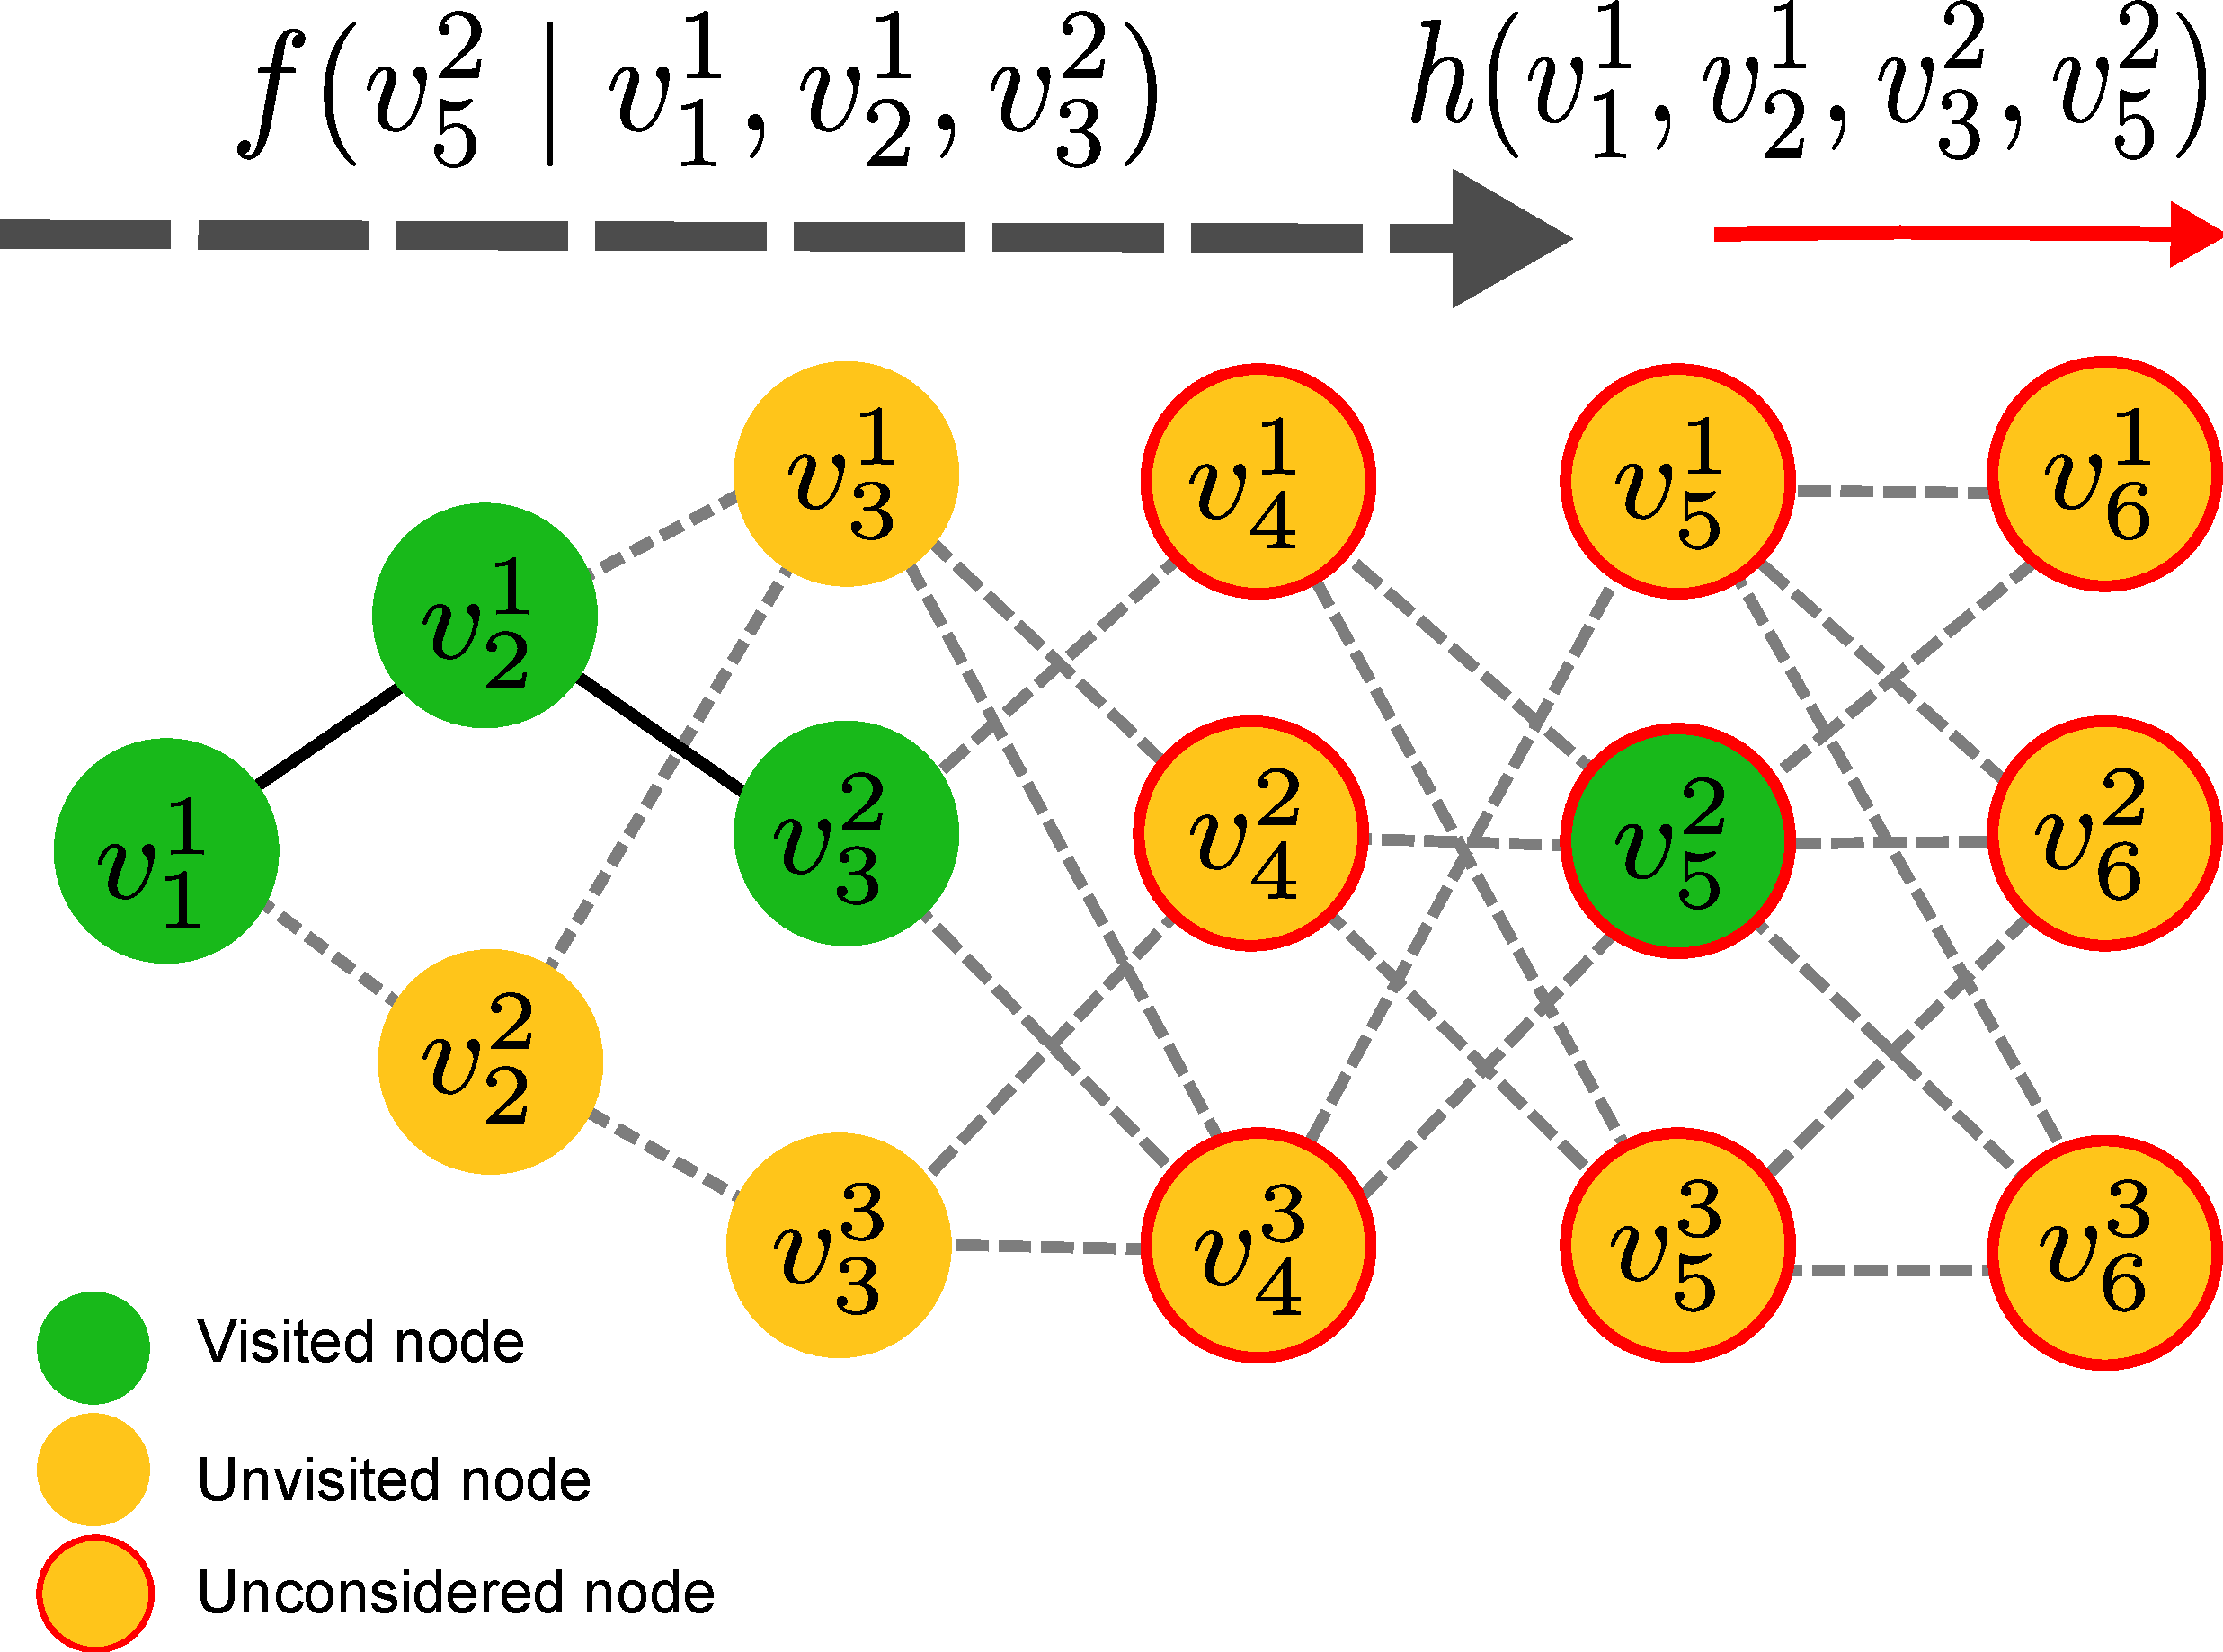
\includegraphics[width=0.5\linewidth]{./images/DefineFuncP.pdf}
\caption{Maximum total reward.}
\label{fig:DefineFuncP}
\end{figure}

By definition of equations \eqref{eq:def_h} and \eqref{eq:def_p}, we have 
\begin{propty}
\label{prop:h2p}
\begin{equation}
\label{eq:h2p}
h( x_{1}, \cdots x_{t'} ) = \max_{x_{t'+1} \in V(t'+1) \land (v_{t'}, x_{t'+1}) \in E} u(x_{t'+1} \mid x_{1}, \cdots x_{t'} ).
\end{equation}
\begin{proof}
The proof is given in Appendix \ref{app:proof_prop_h2p}.
\end{proof}
\end{propty}
After $ x_{t'}, \cdots , x_{1} $ have been visited, there is a vertex $ x^{*}_{t'+1} $ at time $ t' + 1 $ which has the biggest value of maximum total reward in those vertices that are connected with $ x_{t'} $. 
The maximum total reward that is calculated from vertex $ x^{*}_{t'+1} $ with $ x_{1}, \cdots x_{t'} $ visited is equivalent to the maximum future reward of $ x_{t'}, \cdots , x_{1} $.

With defined rewards, we can rewrite equation \eqref{eq:max_2} as
\begin{equation}
\label{eq:max_21}
\hat{x}_{t} = \arg \max_{X_{t}} u(x_{t} \mid x_{1} , \cdots , x_{t-1}).
\end{equation}

%At time $ t $, $ g(x_{t} \mid x_{t-1}, \cdots , x_{1}) $ gives the instant reward of choosing $ x_{t} $ with previous sub-solution $ x_{t-1}, \cdots , x_{1} $ given; $ h(x_{t} , x_{t-1} , \cdots, x_{1} ) $ gives the maximum future reward with choices made from $ 1 $ to $ t $.
If $ u(x_{t} \mid x_{1} , \cdots , x_{t-1}) $ at each step can be calculated correctly at each time step, the solution found can be optimal by Bellmen's \emph{principle of optimality} [\cite{lewis1986optimal}].
Due to the path dependence, calculating future reward at each step is NP-hard.
Brute Force Search exhaustively explores all possible future sub-paths so that it can return the maximum future reward.
Its disadvantage on complexity makes it inapplicable.
Using only a greedy search provides good efficiency but no performance guarantee in this case [\cite{krause2012submodular}], which is discussed in section \ref{sec:related_work}.
Submodularity-based approaches provide useful solutions that have guaranteed performance bounds when sensors/robots can be placed at arbitrary locations, but do not perform well in the presence of path constraints.
In this paper, we import future reward estimation to approximate this optimization calculation process.


\section{A Tree-Expanding Search with Recursive Backtracking}
\label{sec:tree_expanding_search}

In this section, we propose algorithms to solve the submodular orienteering problem on a multi-partite graph.
We use backtracking to estimate the maximum total reward and import an expanding tree to track the search process in an anytime algorithm framework. 

%The path planning problem on a multi-partite graph is equivalent with a search process on a multi-partite graph.
Each solution on the robot path is a sequence of vertices on the multi-partite graph.
We have $ X = ( x_{1}, x_{2} , \cdots , x_{T} ) = ( v_{1}, v_{2} , \cdots , v_{T} ) $.
In a manner of searching the optimal path, we can use the estimated future reward as the heuristic.
%Thus the future reward estimation becomes finding heuristic in a search problem.

Given a start node, any search problem on a graph implicitly derives an expanding tree, the root of which is the start node.
We can always map a multi-partite graph of $ T $ levels to an expanding tree that has fixed depth of $ T $. 

\begin{mydef}[\textbf{Expanding Tree}]
\label{def:expanding_tree}
An expanding tree $ G_{T} = (N, L, T) $ is a tree structure, obtained from a multi-partite graph $ G = (V, E, T) $ so that each node in the expanding tree has only one parent node.
\begin{itemize}
\item $ T $ is the depth of the tree, which is determined by the number of partitions in a multi-partite graph $ G $.
\item $ N $ is the node set. Each $ n_{t}^{i(j)} \in N $ indicates the relevant vertex in the multi-partite graph $ G $, in which $ t $ shows the index of the time partition, $ i $ shows the index of the corresponding vertex from within that partition and $ (j) $ shows the index of a vertex in $ V(t-1) $ that has an out edge to vertex $ i $.
\item $ L $ is the directed link set. $ (n^{i(k)}_{t}, n^{j(i)}_{t+1})  \in L $ is determined by $ (v^{i}_{t}, v^{j}_{t+1} ) \in E $.

\end{itemize}
\end{mydef}

Figure \ref{fig:multipartite_expandingtree} shows an example of how a vertex in a multi-partite graph is mapped to nodes in a corresponding expanding tree. The red edges form both a path on the multi-partite graph and a path on the expanding tree in order to show that paths are preserved in the mapping. 

We can see that each vertex $ v^{i}_{t} $ in the multi-partite graph can map to several nodes $ n^{j(i)}_{t+1} $ in the expanding tree, the number of which is $ deg^{+}(v^{i}_{t})$. Each node $ n^{j(i)}_{t+1} $ in the tree maps to only one vertex, which is denoted as $ v(n^{j(i)}_{t+1}) $.

Each path in an expanding tree is derived from a unique path in a corresponding mutli-partite graph.
For a node $ n_{t}^{i(j)} $, we use $ path(n_{t}^{i(j)}) $ to denote the implicit path from start position to corresponding vertex in the multi-partite graph.
The cardinality of $ path(n_{t}) $ is $ t $.
We have property \ref{prop:path}.
For simplicity of notation, we will use $ n_{t} $ instead of $ n_{t}^{i(j)} $ and $ v_{t} $ instead of $ v_{t}^{i} $ in the following sections. 

\begin{mydef}[\textbf{Complete Path}]
\label{def:complete_path}
A complete path in a path-planning problem with a planning length $ T $, is any path such that
$ | path() | = T  $ .
\end{mydef}

\begin{mydef}[\textbf{Terminal Node}]
\label{def:terminal_node}
A terminal node, defined by $ n_{T} $, is any node at level $ T $ in an expanding tree $ G_{T} = (N, L, T) $ . 
For any node $ n_{T} $, $ path(n_{T}) $ is a complete path by definition.
\end{mydef}

\begin{figure}
\centering
\includegraphics[width=0.4\linewidth]{./images/multipartite_expandingtree.pdf}
\caption{Mapping from a multi-partite graph to an expanding tree.}
\label{fig:multipartite_expandingtree}
\end{figure}

From the mapping between a multi-partite graph and an expanding tree, we can have Property \ref{prop:path}.

\begin{propty}
\label{prop:path}
Each node $ n_{t}^{i(j)} $, which maps to $ v_{t}^{i} $ in a multi-partite graph, implies one and only path from root to node $ n_{t}^{i(j)} $.
We define $ path(n_{t}) = ( n_{1}, n_{2} , \cdots , n_{t} ) $.
Equivalently, $ path(n_{t}) = ( v_{1}, v_{2} , \cdots , v_{t} ) $.
\end{propty}

By Property \ref{prop:orderIndependence}, we can ignore the sequence and denote $ path(n_{t}) = \{ n_{1}, n_{2} , \cdots , n_{t} \} $ as a set.

As shown in Figure \ref{fig:backtracking}, we utilize the structure of a multi-partite graph to back propagate information in estimating future reward. 
The process is given in Algorithm \ref{alg:Backtrack}.

\subsection{Backtracking Algorithm}
\label{subsec:backtrack_algorithm}

For short, we let $ f(x_{t} \mid x_{t'}=v_{t'}, x_{t'-1} = v_{t'-1} , \cdots  , x_{1} = v_{1} ) = f(x_{t} \mid v_{1}, \cdots , v_{t'}) = f(x_{t} \mid path(n_{t'})) $. 

\begin{lem}
\label{lem:submod}
When $ t' < t $, 
\begin{equation}
\label{eq:lem_submod}
f(x_{t} \mid v_{1} , \cdots , v_{t'} ) \geq f(x_{t} \mid v_{1} , \cdots , v_{t'} , \hat{x}_{t'+1} , \cdots , \hat{x}_{t-1}  ). 
\end{equation}
$ \hat{x}_{t-1} , \cdots , \hat{x}_{t'+1} $ indicate any set of vertices that consists of the combinations from partitions $ t'+1 $ to $ t - 1 $ in the multi-partite graph.
\begin{proof}
We have $ \{ v_{1} , \cdots , v_{t'} \} \subseteq \{ \hat{x}_{t'+1} , \cdots , \hat{x}_{t-1} \} \cup \{ v_{1} , \cdots , v_{t'} \} $.
By the submodular property, see in equation \eqref{eq:cond_submod_prop}, equation \eqref{eq:lem_submod} follows. 
\end{proof}
\end{lem}

\begin{figure}
\centering
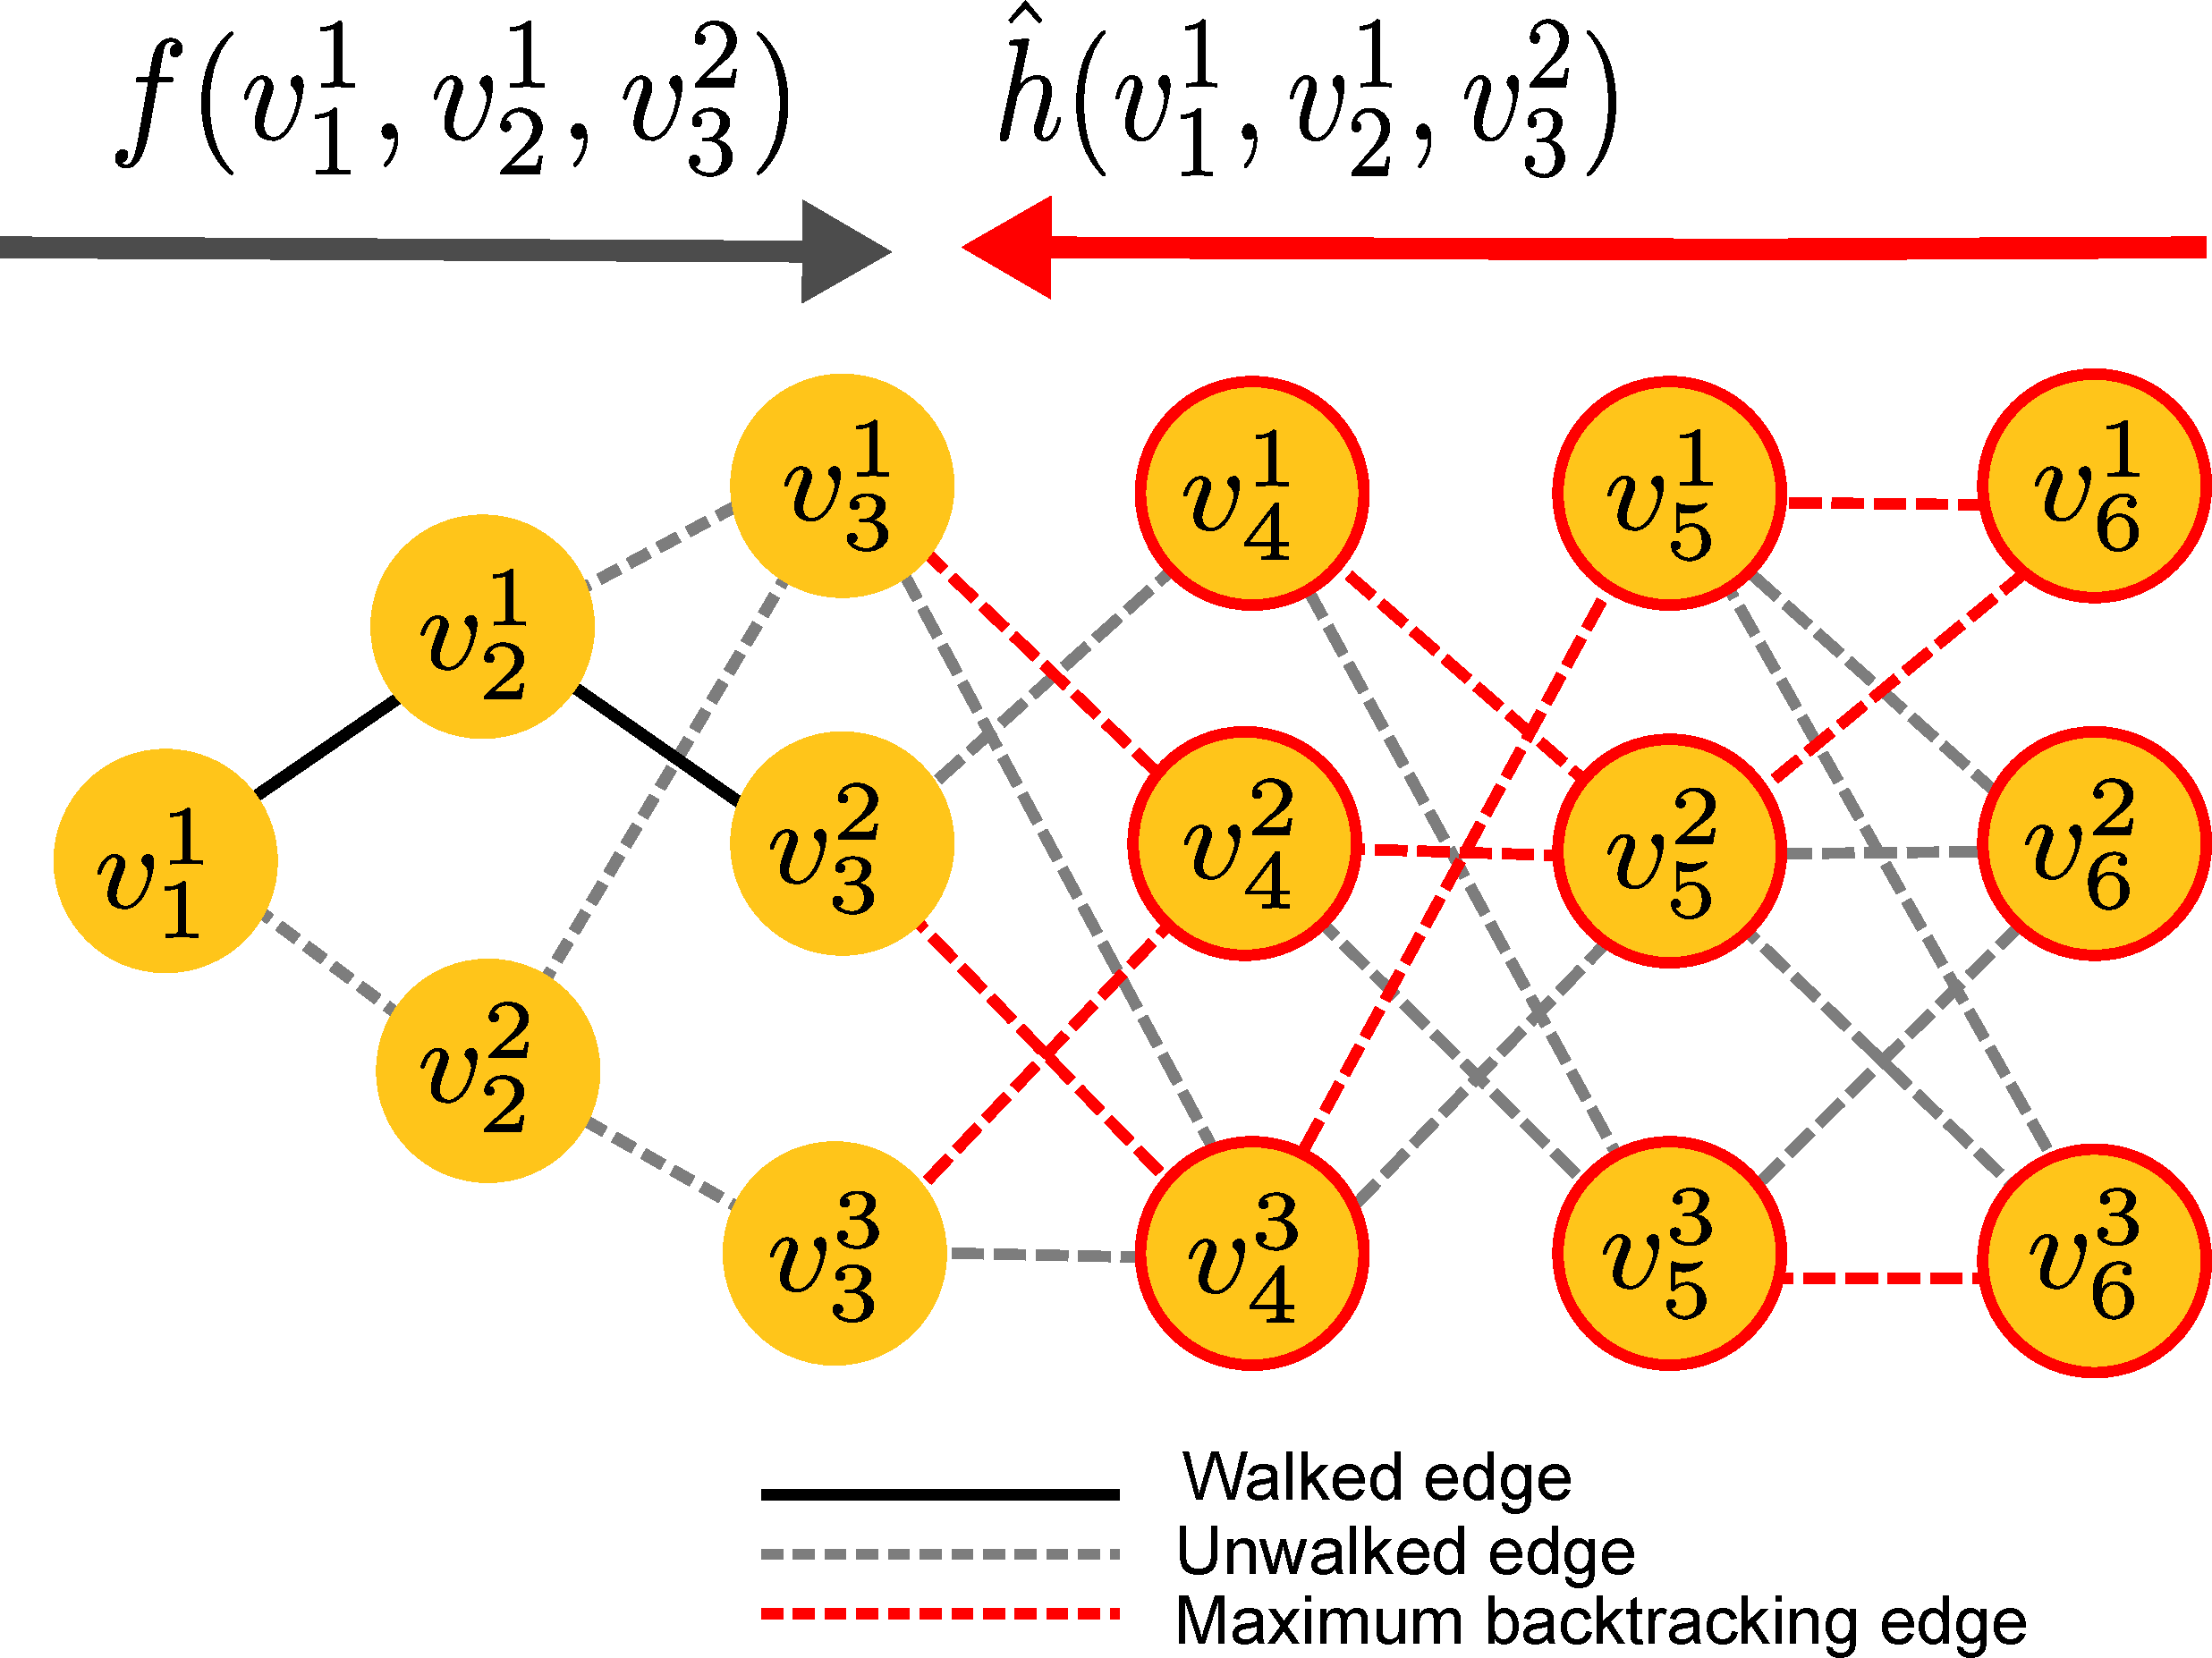
\includegraphics[width=0.5\linewidth]{./images/backtracking.pdf}
\caption{Backtracking process.}
\label{fig:backtracking}
\end{figure}

When we have $ \{ v_{1} , \cdots , v_{t'} \} $ visited, Algorithm \ref{alg:Backtrack} gives an estimated maximum future reward $ \hat{h}( v_{1} , \cdots , v_{t'} ) $. 
 
\begin{algorithm}
\caption{ $ \mathbf{BT}( \{ v_{1} , \cdots , v_{t'} \}, G ) $ - Backtracking }
\label{alg:Backtrack}
\begin{algorithmic}[1]
\REQUIRE
a sub-path $ \{ v_{1} , \cdots , v_{t'} \} $, and multi-partite graph $ G = ( V, E, T ) $
\ENSURE $ \hat{h}( v_{1} , \cdots , v_{t'} ) $ \\
\FOR{ $ t=T:-1:t'+1 $ }
\FOR{ $ v_{t} \in V(t) $}
\IF {$ t == T $}
\STATE $ \hat{u}(v_{T} \mid v_{1} , \cdots , v_{t'} ) = f(v_{T} \mid v_{1} , \cdots , v_{t'} ) $
\ELSE
\STATE $ \hat{h}( v_{1} , \cdots , v_{t'},  v_{t} ) = \max_{ { x_{t+1} \in V(t+1) } \land { (v_{t}, x_{t+1}) \in E } } \hat{u}(x_{t+1} \mid v_{1} , \cdots , v_{t'} ) $
\STATE $ \hat{u}(v_{t} \mid v_{1} , \cdots , v_{t'} ) = f(v_{t} \mid v_{1} , \cdots , v_{t'} ) + \hat{h}( v_{1} , \cdots , v_{t'} , v_{t}) $
\ENDIF
\ENDFOR
\ENDFOR
\STATE  $ \hat{h}( v_{1} , \cdots , v_{t'} ) = \max_{ {x_{t'+1} \in V(t'+1)} \land {(v_{t'}, x_{t'+1}) \in E} } \hat{u}(x_{t'+1} \mid v_{1} , \cdots , v_{t'} ) $
\RETURN $ \hat{h}( v_{1} , \cdots , v_{t'} )  $
\end{algorithmic}
\end{algorithm}
%Backtrack process provides all the possible future rewards of next step $ \hat{R}^{max}_{future}(x_{path(v).length+1} \mid path(v) ) $. Selecting the maximum, we can used this as the estimation on future reward of node $ v $, $ est_{max}(R^{max}_{future}(v)) $.

Algorithm \ref{alg:Backtrack} estimates the maximum total rewards of the vertices in a backward manner, which starts from time partition $ V(T) $ back to $ V(t'+1) $.
For each vertex $ v(t) $, the estimated maximum total reward $ \hat{u}(x_{t'+1} \mid v_{1} , \cdots , v_{t'} ) $ is a sum of the estimated instant reward and the estimated future reward.
The estimated instant reward is calculated by $ f(v_{t} \mid v_{1} , \cdots , v_{t'} ) $ .
The estimated future reward $ \hat{h}( v_{1} , \cdots , v_{t'} , v_{t}) $ is calculated by the following steps.
\begin{enumerate}
\item Find the vertex that has the biggest value of the estimated maximum total reward from the vertices in partition $ V(t+1) $ that are connected with $ v(t) $;
\item Take its estimated maximum total reward as the maximum future reward of $ v(t) $.
\end{enumerate}

We notice that there is an important property of the ``Backtracking'' defined in Algorithm \ref{alg:Backtrack}, which gives Lemma \ref{lem:underestimate}.

\begin{lem}
\label{lem:underestimate}
``Backtracking" in Algorithm \ref{alg:Backtrack} will never underestimate the maximum future reward, which means 
\begin{equation}
\label{eq:overestimate}
\hat{h}( v_{1} , \cdots , v_{t'} ) \geq h( v_{1} , \cdots , v_{t'} ).
\end{equation}
\begin{proof}

%By property \ref{prop:path}, we know that $ path(n_{t'}) $ defines a set of vertices in a sub-path $ \{ v_{1}, v_{2} , \cdots , v_{t'} \} $.
%Thus we need to look at maximum future reward $ h() $ and estimated maximum future reward $ \hat{h}() $ after $ \{ v_{1}, v_{2} , \cdots , v_{t'} \} $ visited. 

As defined in line 7 of Algorithm \ref{alg:Backtrack}, we can have
\begin{equation}
\label{eq:hatp_def}
\hat{u}( x_{t} \mid v_{1} , \cdots , v_{t'} ) = g(x_{t} \mid v_{1} , \cdots , v_{t'} ) + \hat{h}(v_{1} , \cdots , v_{t'}, x_{t} ).
\end{equation}
Similarly, as defined in line 6 of Algorithm \ref{alg:Backtrack}, we can have
\begin{equation}
\label{eq:hath2hatp}
\hat{h}( v_{1} , \cdots , v_{t'} ) = \max_{x_{t'+1} \in V(t'+1) \land (v_{t'}, x_{t'+1}) \in E} \hat{u}(x_{t'+1} \mid v_{1} , \cdots , v_{t'} ).
\end{equation}

By replacing the $ \hat{h}( v_{1} , \cdots , v_{t'} ) $ in equation \eqref{eq:overestimate} with equation \eqref{eq:hath2hatp} and replacing the $ h( v_{1} , \cdots , v_{t'} ) $ in equation \eqref{eq:overestimate} with equation \eqref{eq:h2p}, we can have
\begin{equation}
\label{eq:inductEnd}
\begin{aligned}
\max_{x_{t'+1} \in V(t+1) \land (v_{t'}, x_{t'+1}) \in E } \hat{u}(x_{t'+1} \mid v_{1} , \cdots , v_{t'} ) \geq \max_{x_{t'+1} \in V(t+1) \land (v_{t'}, x_{t'+1}) \in E } u(x_{t'+1} \mid v_{1} , \cdots , v_{t'} ).
\end{aligned}
\end{equation}

We prove equation \eqref{eq:overestimate} by using equation \eqref{eq:inductEnd} as an equivalence to prove.

By Property \ref{prop:u2gh_2}, we can express the maximum total reward in a form that approximates the steps in Algorithm \ref{alg:Backtrack} to facilitate the comparison.
We have, for any given time $ t > t' $,
\begin{equation}
\label{eq:def_g_2}
u( x_{t} \mid v_{1} , \cdots , v_{t'} ) = f( x_{t} \mid \tilde{x}_{t+1}, \cdots \tilde{x}_{T}, v_{1} , \cdots , v_{t'} ) +  \max_{x_{t+1} \in V(t+1) \land ( x_{t}, x_{t+1} ) \in E } u( x_{t+1} \mid v_{1} , \cdots , v_{t'} ).
\end{equation}

In estimating the total reward using Algorithm \ref{alg:Backtrack}, $ \{ \tilde{x}_{t+1}, \cdots , \tilde{x}_{T} \} $ is not predicted to apply into calculating instant reward of $ x_{t} $.
We have estimated maximum total reward$ \hat{u}(x_{t} \mid v_{1} , \cdots , v_{t'} ) $ as 
\begin{equation}
\label{eq:defHatG}
\begin{aligned}
\hat{u}( x_{t} \mid v_{1} , \cdots , v_{t'} ) = f( x_{t} \mid v_{1} , \cdots , v_{t'} ) + \max_{ x_{t+1} \in V(t+1) \land ( x_{t}, x_{t+1} ) \in E } \hat{u}( x_{t+1} \mid v_{1} , \cdots , v_{t'} ).
\end{aligned}
\end{equation}

Like the procedure of backtracking, we import an proof by induction from $ T $ back to $ t' + 1 $.

\textbf{Initial}

At time $ T $, we have
\begin{equation}
\label{eq:eqT1}
\begin{aligned}
u( x_{T} \mid  v_{1} , \cdots , v_{t'} ) = f( x_{T} \mid v_{1} , \cdots , v_{t'} ),
\end{aligned}
\end{equation}
and
\begin{equation}
\label{eq:eqT2}
\begin{aligned}
\hat{u}( x_{T} \mid v_{1} , \cdots , v_{t'} ) = f( x_{T} \mid v_{1} , \cdots , v_{t'} ).
\end{aligned}
\end{equation}

Combining equations \eqref{eq:eqT1} and \eqref{eq:eqT2}, we have
\begin{equation}
\label{eq:inductionInit}
\begin{aligned}
\forall x_{T} \in V(T), \hat{u}( x_{T} \mid v_{1} , \cdots , v_{t'} ) = u( x_{T} \mid v_{1} , \cdots , v_{t'} ).
\end{aligned}
\end{equation}

\textbf{Induction}

At any time $ t > t' $, assume that
\begin{equation}
\label{eq:inductionAssumption}
\begin{aligned}
\forall x_{t+1} \in V(t+1), \hat{u}(x_{t+1} \mid v_{1} , \cdots , v_{t'} ) \geq u(x_{t+1} \mid v_{1} , \cdots , v_{t'} ).
\end{aligned}
\end{equation}

Looking at the difference at time step $ t $ with  $ \hat{u}(\cdot) $ and $ u(\cdot) $ by equations \eqref{eq:def_g_2} and \eqref{eq:defHatG}, for any $ x_{t} $ we have

\begin{equation}
\label{eq:extendDifference}
\begin{aligned}
& \hat{u}( x_{t} \mid v_{1} , \cdots , v_{t'} ) - u(x_{t} \mid v_{1} , \cdots , v_{t'} ) \\
& = \left[( f( x_{t} \mid v_{1} , \cdots , v_{t'} ) + \max_{x_{t+1} \in V(t+1) \land (x_{t}, x_{t+1}) \in E } \hat{u}( x_{t+1} \mid v_{1} , \cdots , v_{t'} ) \right]  \\
& - \left[  f( x_{t} \mid v_{1} , \cdots , v_{t'}, \tilde{x}_{t+1}, \cdots \tilde{x}_{T} ) +  \max_{x_{t+1} \in V(t+1) \land ( x_{t}, x_{t+1} ) \in E } u( x_{t+1} \mid v_{1} , \cdots , v_{t'} ) \right]  \\
& = \left[ f(x_{t} \mid v_{1} , \cdots , v_{t'} ) - f(x_{t} \mid v_{1} , \cdots , v_{t'}, \tilde{x}_{t+1}, \cdots \tilde{x}_{T} ) \right] \\
& + \left[ \max_{ x_{t+1} \in V(t+1) \land ( x_{t}, x_{t+1} ) \in E } \hat{u}( x_{t+1} \mid v_{1} , \cdots , v_{t'} ) - \max_{x_{t+1} \in V(t+1) \land ( x_{t}, x_{t+1} ) \in E } u( x_{t+1} \mid v_{1} , \cdots , v_{t'} ) \right] .
\end{aligned}
\end{equation}

We can see that if 
\begin{equation}
\label{eq:inductionGEQ1}
f( x_{t} \mid v_{1} , \cdots , v_{t'} ) - f(x_{t} \mid v_{1} , \cdots , v_{t'}, \tilde{x}_{t+1}, \cdots \tilde{x}_{T} ) \geq 0,
\end{equation}
and
\begin{equation}
\label{eq:max_delta}
\max_{ x_{t+1} \in V(t+1) \land ( x_{t}, x_{t+1} ) \in E } \hat{u}( x_{t+1} \mid v_{1} , \cdots , v_{t'} ) - \max_{ x_{t+1} \in V(t+1) \land ( x_{t}, x_{t+1} ) \in E } u( x_{t+1} \mid v_{1} , \cdots , v_{t'} ) \geq 0.
\end{equation}
are both true, we can have
\begin{equation}
\label{eq:extendDifference_geq_0}
\hat{u}( x_{t} \mid v_{1} , \cdots , v_{t'} ) - u( x_{t} \mid v_{1} , \cdots , v_{t'} ) \geq 0
\end{equation}
proved. Thus we will prove equation \eqref{eq:inductionGEQ1} and equation \eqref{eq:max_delta} respectively.

By Lemma \ref{lem:submod}, we can prove equation \eqref{eq:inductionGEQ1} directly.

Then we are going to prove equation \eqref{eq:max_delta} is also true.

Let 
\begin{equation}
\label{eq:arg_x_a}
x^{a}_{t+1} = \arg \max_{ x_{t+1} \in V(t+1) \land ( x_{t}, x_{t+1} ) \in E} \hat{u}( x_{t+1} \mid v_{t'} , \cdots , v_{1} )
\end{equation}
and 
\begin{equation}
\label{eq:arg_x_b}
x^{b}_{t+1} = \arg \max_{ x_{t+1} \in V(t+1) \land ( x_{t}, x_{t+1}) \in E } u( x_{t+1} \mid v_{1} , \cdots , v_{t'} ). 
\end{equation}

$ x^{a}_{t+1} $ and $ x^{b}_{t+1} $ can be either same or different. Both two belong to same set satisfying $ x_{t+1} \in V(t+1) \land (x_{t}, x_{t+1}) \in E $.

Since $ x^{a}_{t+1} $ is the answer to $ \arg \max \hat{u}(\cdot) $, we have
\begin{equation}
\label{eq:bigger1}
\begin{aligned}
\hat{u}( x^{a}_{t+1} \mid v_{1} , \cdots , v_{t'} ) \geq \hat{u}( x^{b}_{t+1} \mid v_{1} , \cdots , v_{t'} ).
\end{aligned}
\end{equation}


By equation \eqref{eq:inductionAssumption},
\begin{equation}
\label{eq:bigger2}
\begin{aligned}
\hat{u}( x^{b}_{t+1} \mid v_{1} , \cdots , v_{t'} ) \geq u( x^{b}_{t+1} \mid v_{1} , \cdots , v_{t'} ).
\end{aligned}
\end{equation}

Combining equations \eqref{eq:bigger1} and \eqref{eq:bigger2} using transitivity, we have 
\begin{equation}
\label{eq:bigger_trans}
 \hat{u}( x^{a}_{t+1} \mid v_{1} , \cdots , v_{t'} ) \geq  u ( x^{b}_{t+1} \mid v_{1} , \cdots , v_{t'} ).
\end{equation}

By the definitions in equations \eqref{eq:arg_x_a} and \eqref{eq:arg_x_b}, equation \eqref{eq:bigger_trans} is equivalent to equation \eqref{eq:max_delta}. Thus equation \eqref{eq:max_delta} is true.

With equations \eqref{eq:inductionGEQ1} and \eqref{eq:max_delta}, we have
\begin{equation}
\label{eq:inductConclusion}
\forall x_{t} \in V(t), \hat{u}( x_{t} \mid v_{1} , \cdots , v_{t'} ) \geq u( x_{t} \mid v_{1} , \cdots , v_{t'} ).
\end{equation}

Thus, we have
\begin{equation}
\label{eq:induction}
\begin{aligned}
\forall x_{t+1} \in V(t+1), \hat{u}( x_{t+1} \mid v_{1} , \cdots , v_{t'} ) \geq u( x_{t+1} \mid v_{1} , \cdots , v_{t'} )  \\
\Rightarrow  \forall x_{t} \in V(t), \hat{u}( x_{t} \mid v_{1} , \cdots , v_{t'} ) \geq u( x_{t} \mid v_{1} , \cdots , v_{t'} ).
\end{aligned}
\end{equation}

\textbf{Conclusion}

Using equations \eqref{eq:inductionInit} and \eqref{eq:induction}, we can apply induction from $ T $ to $ t'+1 $ to get
\begin{equation}
\label{eq:inductionResult}
\forall x_{t'+1} \in V(t'+1), \hat{u}( x_{t'+1} \mid v_{1} , \cdots , v_{t'} ) \geq u( x_{t'+1} \mid v_{1} , \cdots , v_{t'} ).
\end{equation}

Applying $ max(\cdot) $ operator on equation \eqref{eq:inductionResult} gets equation \eqref{eq:inductEnd}.
Equation \eqref{eq:inductEnd} has been proved, which means that equation \eqref{eq:overestimate} stands.
So we arrive to the conclusion that ``Backtracking" in Algorithm \ref{alg:Backtrack} will never underestimate the future reward.

\end{proof}
\end{lem}

\subsection{Tree Expanding Search}
\label{subsec:tree_expanding_search}

Recall that $ path(n_{t}) $ of a node $ n_{t} $ in the expanding tree $ G_{T} $ maps to a unique path in the multi-partite graph $ G $ in Property \ref{prop:path}.
We model the process of path search on the multi-partite graph $ G $ as a tree expanding process.
A backtracking process can generate estimated maximum future rewards for all the vertices in the unvisited partitions.
Since the backtracking process does not guarantee that there is no bias on the estimation, the first complete path created in the expanding tree might not be the optimal solution.
If the search does not stop at finding one complete solution, the expanding tree $ G_{T} $ can be used to track whether a vertex in a path on the multi-partite graph $ G $ has been explored and to store its estimated rewards.
Adding a node $ n^{i(j)}_{t} $ means that a sub-path $ path( n^{i(j)}_{t} ) $ has been explored on the multi-partite graph $ G $.
``Expanding'' a node includes adding the children of node $ n_{t} $ to our $ G_{T} $ data structure and storing the estimated rewards of a sub-path $ path(n_{t}) $ in node $ n_{t} $ by ``backtracking''.

Here we assign a state to each node $ n_{t} $ to facilitate the history tracking in the search process. 
There are three types of states:
\begin{description}
\item [New] a node has been created but not expanded;
\item [Expanded] a node that has all child nodes created;
\item [Frozen] a node that has been created but will not be expanded.
\end{description}

In order to have a better approximation to the true value of $ h() $, we will call Algorithm \ref{alg:Backtrack} to estimate the maximum future reward for the newly added nodes
\footnote{A proof on that estimating maximum future reward with newly added vertex provides a better approximation to the $ h() $ is given in Appendix \ref{app:better_approximation} }. 
Integrating ``recursive backtracking" into a ``node expanding'' process, we propose Algorithm \ref{alg:RecursiveBacktrack}.
Since each expanding node indicates a sub-path from the root node, Algorithm \ref{alg:RecursiveBacktrack} can start from any expanding node $ n_{t'} $ and concatenate the sub-path $ path(n_{t'}) $ to generate a complete path solution.

\begin{algorithm}
\caption{ $ \mathbf{NERB}( n_{t'}, G, G_{T} ) $ - Node Expanding with Recursive Backtracking }
\label{alg:RecursiveBacktrack}
\begin{algorithmic}[1]
\REQUIRE 
Expanding Node $ n_{t'} $, Multi-partite graph $ G = (V, E, T) $, Expanding tree $ G_{T} = (N, L, T) $
\ENSURE $ solution $ of a complete path
\STATE $ solution = path(n_{t'}) $ 
\FOR{ $ t=t':1:T-1 $ }
\STATE  Expand node $ n_{t'} $ to get $ child(n_{t'}) $
\STATE  $ n_{t'}.state = \mbox{\emph{Expanded}} $
\STATE  $ child(n_{t'}) = \{ n_{t'+1} \mid v(n_{t'+1}) \in V(t'+1) \land (v(n_{t'}), v(n_{t'+1})) \in E  \} $
\FOR{ $ n_{t'+1} $ in $ child(n_{t'}) $ }
\STATE  calculate $ f(path(n_{t'+1})) $
\STATE  $ \hat{h}(path(n_{t'+1})) = \mathbf{BT}( path(n_{t'+1}) , G ) $
\ENDFOR
\STATE  $ \hat{n}_{t'+1} = \arg \max_{n_{t'+1} \in child(n_{t'})} \hat{h}(path(n_{t'+1})) $
\STATE  $ solution = solution \bigcup \{ \hat{n}_{t'+1} \} $
\ENDFOR 
\RETURN $ solution $
\end{algorithmic}
\end{algorithm}

In Algorithm \ref{alg:RecursiveBacktrack}, $ child() $ is defined for a set of the children nodes of an expanding node $ n_{t'} $, which is generated from a set of all the vertices in $ V(t'+1) $ that are connected with $ v(n_{t'}) $.
We are able to get a solution of a complete path using Algorithm \ref{alg:RecursiveBacktrack} by recursively estimate $ \hat{h}(path(n_{t})) $ at each time step $ t $.
Each single run of Algorithm \ref{alg:RecursiveBacktrack} reaches a terminal node in the expanding tree.
By the heuristic from backtracking estimation, a complete path can be optimal or near optimal.
The optimality depends on how the correctness on estimating maximum future reward influence the optimal solution search.

\subsection{Anytime Algorithm Framework}
\label{subsec:anytime_algorithm_framework}

The tree expanding search naturally implies an anytime algorithm framework. 
In this section, we formalize the tree expanding search as an anytime algorithm framework.
It means that we have a solution from the first single call of Algorithm \ref{alg:RecursiveBacktrack} and continues to search for a potential better solution. 

In avoid of an exhaustive search, we propose a node freeze process to prune those nodes that are impossible to reach an optimal terminal node. ``Freezing" a node means never exploring the child nodes of a node, which works in a similar way with pruning in search. 

\begin{figure}
\centering
\includegraphics[width=0.7\linewidth]{./images/freeze_process.pdf}
\caption{Node freeze process.}
\label{fig:freeze_process}
\end{figure}

By Lemma \ref{lem:underestimate}, if the estimated maximum total reward of a node in an expanding tree is smaller than the total reward of current best path, it is impossible that this node locates in a complete path that has bigger total reward.
We are not interested with any descendant nodes of this node, thus freeze this node.
A node is frozen means that the sub-tree structure from this node will never be explored.
The node freeze process is used to update the states of the nodes in an expanding tree, which is given in Algorithm \ref{alg:FreezeNode}.

\begin{algorithm}
\caption{Node Freeze}
\label{alg:FreezeNode}
\begin{algorithmic}[1]
\REQUIRE 
an expanding tree $ G_{T} = (N, L, T) $, the current best terminal node $ \hat{n}^{*}_{T} $
\STATE $ \theta = f(path(\hat{n}^{*}_{T})) $
\FOR{$ n_{t} \in N $ \AND $ n_{t}.state == \mbox{\emph{New}} $}
\IF{ $ \hat{h}(path(n_{t})) + f(path(n_{t})) \leq \theta $ }
\STATE $ n_{t}.state = \mbox{\emph{Frozen}} $
\ENDIF
\ENDFOR
\end{algorithmic}
\end{algorithm}

After all the sub-procedures given, we can form the ``anytime algorithm framework''.
An expanding tree starts from a structure with only a root node - start position.
When a node is initially created, the state of the node is \emph{New}.
Algorithm \ref{alg:Backtrack} expands a node by creating all its child nodes and changes the state of the node to \emph{Expanded}.
The estimating maximum total rewards of all child nodes will also be calculated and stored.
After first run of Algorithm \ref{alg:RecursiveBacktrack}, an optimal or near-optimal complete path is obtained.
When a new complete path has been found, a freeze process defined in \ref{alg:FreezeNode} will be executed by checking estimated total rewards stored in each nodes in the state of \emph{New}.
If there is enough calculating time budget that allows a next run of search, the framework will find a node $ n_{t} $ that has the largest estimated total reward $ \hat{h}(path(n_{t})) + f(path(n_{t})) $.
Starting from this node, a next call to Algorithm \ref{alg:RecursiveBacktrack} will find another complete path.
This anytime algorithm framework is stopped by some stopping criteria or that there is no node of state $ New $ left.
The process is given in Algorithm \ref{alg:Anytime}.

\begin{algorithm}
\caption{Anytime Algorithm Framework}
\label{alg:Anytime}
\begin{algorithmic}[1]
\REQUIRE 
Expanding Tree $ G_{T} = (N, L, T) $, and multi-partite graph $ G = (V, E, T) $;
\STATE Initial expanding tree $ G_{t}(N, L, T) $ with $ v_{1} $ as root node
\STATE $ maxPath = NULL $, $ newPath = NULL $
\STATE $ n' = G_{T}.root $
\WHILE { $ n' != NULL $ }
\STATE $ newPath = \mathbf{NERB}( n', G, G_{T} ) $
\IF {$ (f(newPath) > f(maxPath))  $}
\STATE $ maxPath = newPath $
\STATE post $ maxPath $
\ENDIF
\STATE Call ``Node Freeze" of Algorithm \ref{alg:FreezeNode}
\STATE $ n' = \arg \max_{ \{n \mid n \in N \land n.state == \mbox{\emph{New}} \} } \hat{h}(path(n)) $
\ENDWHILE 
\end{algorithmic}
\end{algorithm}

We propose that theorem \ref{thm:optimal} stands on the anytime algorithm framework in Algorithm \ref{alg:Anytime}.

\begin{thm} 
\label{thm:optimal}
The anytime algorithm framework in Algorithm \ref{alg:Anytime} can always find an optimal solution given enough run time.
\begin{proof}

Finding the optimal solution equals to reaching a terminal node in the optimal path of the expanding tree.
Since Algorithm \ref{alg:Anytime} keeps expanding new nodes till that there is no node in state \emph{New}, as long as any node in the optimal path will never be frozen, the search will reach the optimal terminal node.

Assume that one of the node $ n^{*}_{t} $ in the optimal path can be frozen. It means that 
\begin{equation}
\label{eq:contra_assumption}
\hat{h}(path(n^{*}_{t})) + f(path(n^{*}_{t})) \leq f(path(n'_{T})),
\end{equation}
in which $ n'_{T} $ is another terminal node but not optimal terminal node.
As a result, when $ n'_{T} $ has been reached, it will freeze node $ n^{*}_{t} $. 

However, as node $ n^{*}_{t} $ is in a path to an optimal terminal node, $ f(path(n^{*}_{t})) + h(path(n^{*}_{t})) > f(path(n'_{T})) $.
Also we have $ f(path(n^{*}_{t})) + \hat{h}(path(n^{*}_{t})) \geq f(path(n^{*}_{t})) + h(path(n^{*}_{t})) $ by Lemma \ref{lem:underestimate}.
Thus we have $ f(path(n^{*}_{t})) + \hat{h}(path(n^{*}_{t}) > f(path(n'_{T})) $. It contradict with equation \eqref{eq:contra_assumption}.

Therefore, an node in a path to an optimal terminal node will never be frozen by any non-optimal terminal node.
It guarantees that an optimal terminal node will always be reached given enough run times.
It means that the anytime algorithm framework in Algorithm \ref{alg:Anytime} can always find an optimal solution.

\end{proof}
\end{thm}






\section{Summary}
\label{sec:summary}

In this paper, we use a human path to form a path constraint and seek to maximize the information gathered by a robot gathered in a search task.
The resulting information maximization path planning is identified as a constrained submodular orienteering problem on a multi-partite graph.
We present an anytime algorithm that used a planning heuristic based on backtracking to efficiently find a high quality path.
We use a node freeze process to avoid an exhaustive search, yet we prove that this process always preserves the ability of the algorithm to find an optimal solution.
We have also shown empirically that this approach substantially reduces the complexity of the resulting search.

\bibliographystyle{IEEEtran}
\bibliography{reference}

\section*{Appendix}

\subsection{ISS-Lyapunov function}
\label{sec:iss_lyapunov:func}

Using the definitions of a $ K $-function and a $ KL $-function in Section \ref{sec:system}
we can define a ISS-Lyapunov function as follows,
%\begin{itemize}
%\item 
an ISS-Lyapunov function $ V : \mathbb{R}^{n} \rightarrow \mathbb{R}_{\geq 0} $ satisfies:
\begin{enumerate}
\item $ \exists \alpha_{1}, \alpha_{2} \in \mathbb{K} $ such that 
$ \forall \xi \in \mathbb{R}^{n} $ , $ \alpha_{1} ( | \xi | ) \leq V( \xi ) \leq \alpha_{2}  ( | \xi | ) $.
\item $ \exists \alpha_{3} \in \mathbb{K}_{\infty} , \sigma \in \mathbb{K} $ such that $ \forall \xi \in \mathbb{R}^{n}, \forall \mu \in \mathbb{R}^{m} $,$  V( f( \xi, \mu ) ) - V( \xi ) \leq - \alpha_{3} ( | \xi | ) + \sigma ( | \mu | ) $. 
\end{enumerate}

\subsection{Proof of Theorem \ref{thm:iss}}
\label{sec:thm:iss:proof}
		
\begin{proof} 
Let $ P $ be an identity matrix.
As $ | \lambda_{\max} ( A(k) ) | < 1 $, we have
%\begin{equation}
%\nonumber
$
\lVert A^{T}(k) P A(k) \rVert \leq \lVert P \rVert \lVert A(k) \rVert^{2} \leq \lVert P \rVert | \lambda_{\max} ( A(k) ) |^{2} $ $  <  \lVert P \rVert .
$
%\end{equation}
Because $ P $ is an identity matrix it is positive definite, and thus $ A^{T}(k) P A(k) $ is positive definite or positive semi-definite by definition.
So by positive definite ordering we have $ A^{T}(k) P A(k) < P $.
		
Let $ -Q(k) = A^{T}(k) P A(k) - P $. Since $ A^{T}(k) P A(k) < P $ then $ - Q(k) < 0 $ furthermore $ \exists Q' \forall k, Q(k) > Q' > 0 $. 
		
By the Lemma 3.5 in \cite{Jiang2001857}, if we can show that a proposed positive definite Lyapunov function is an ISS-Lyapunov function, then the system is ISS.
		
Define a Lyapunov function
\begin{equation}
\label{eq:lyapunov_v}
V( X(k) ) = X^{T} (k) P X(k).
\end{equation}
We can have
$
\lambda_{min}(P) | X(k) |^{2} \leq V( X(k) )\leq \lambda_{max}(P) | X(k) |^{2}
$ and $ \lambda_{min}(P) = \lambda_{max}(P) $.
		
Let $ \alpha_{1} ( \xi )= \lambda_{min} \xi^{2} $
and 
$ \alpha_{2} ( \xi )= \lambda_{max} \xi^{2} $,
we have $ V(x) $ satisfying condition 1 of the ISS-Lyapunov function definition.
		
By applying equation \eqref{eq:pso_up_linalg_simp} to $ V( X(k+1) ) - V( X(k) ) $, we have
\begin{equation}
\label{eq:lyapunov_delta2}
\begin{aligned}
& V( X(k+1) ) - V( X(k) ) \\
%	= & - X^{T}(k) [ A^{T}(k) P A(k) - P ] X(k) + 2 X^{T}(k)  A^{T}(k) P B(k) U(k) \\
%	& + U^{T}(k) B^{T}(k) P B(k) U(k) \\
%	\leq & - X^{T}(k) Q' X(k) + 2 X^{T}(k)  A^{T}(k) P B(k) U(k) \\
%	& + U^{T}(k) B^{T}(k) P B(k) U(k) \\
%	\leq & - \lambda_{min}(Q') | X(k) |^{2} + 2  \lVert A^{T}(k) P B(k) \rVert  U(k) | | X(k) | \\
%	& + \lVert B^{T}(k) P B(k) \rVert | U(k) |^{2}.
= & [ X^{T}(k)  A^{T}(k) + U^{T}(k) B^{T}(k) ] P [ A(k) X(k) + B(k) U(k) ] \\ & - X^{T}(k) P X(k) \\
= & X^{T}(k)  A^{T}(k) P A(k) X(k) +  X^{T}(k)  A^{T}(k) P B(k) U(k) \\
& + U^{T}(k) B^{T}(k) P A(k) X(k) + U^{T}(k) B^{T}(k) P B(k) U(k) \\ & - X^{T}(k) P X(k) \\
\end{aligned}
\end{equation}
As $ P $ is identity matrix, it is symmetric, thus
\begin{equation}
[ X^{T}(k)  A^{T}(k) P B(k) U(k) ]^{T} =  U^{T}(k) B^{T}(k) P A(k) X(k).
\end{equation}
$ V( X(k+1) ) , V( X(k) ) \in \mathbb{R} $, 
we have $ X^{T}(k)  A^{T}(k) P B(k) U(k) $ and $  U^{T}(k) B^{T}(k) P A(k) X(k) $ are both real value (like $ 1 \times 1 $ matrix).
Thus, 
\begin{equation}
 X^{T}(k)  A^{T}(k) P B(k) U(k) =   U^{T}(k) B^{T}(k) P A(k) X(k) .
\end{equation}
We then have
\begin{equation}
\label{eq:lyapunov_delta3}
\begin{aligned}
& V( X(k+1) ) - V( X(k) ) \\
= & - X^{T}(k) [ A^{T}(k) P A(k) - P ] X(k) \\
& + U^{T}(k) B^{T}(k) P B(k) U(k)  \\
& + 2 X^{T}(k)  A^{T}(k) P B(k) U(k) \\
\leq & - X^{T}(k) Q' X(k)  + U^{T}(k) B^{T}(k) P B(k) U(k) \\
& + 2 X^{T}(k)  A^{T}(k) P B(k) U(k) \\
\end{aligned}
\end{equation}

By applying matrix norm, we have
\begin{equation}
\begin{aligned}
& V( X(k+1) ) - V( X(k) ) \\
\leq & - \lambda_{min}(Q') | X(k) |^{2}  + | B^{T}(k) P B(k) | | U(k) |^{2} \\
& + 2  | A^{T}(k) P B(k) | | U(k) | | X(k) | \\
= & - \frac{1}{2} \lambda_{min}(Q') | X(k) |^{2} + | B^{T}(k) P B(k) | | U(k) |^{2} \\
& - \frac{1}{2} \lambda_{min}(Q') | X(k) |^{2} + 2  | A^{T}(k) P B(k) | | U(k) | | X(k) |  \\
= & - \frac{1}{2} \lambda_{min}(Q') | X(k) |^{2} \\
& + \left( \frac{2 | A^{T}(k) P B(k) |^{2}}{ ( \lambda_{min}(Q') )^{2} } + | B^{T}(k) P B(k) |  \right) | U(k) |^{2} \\
& - \frac{1}{2} \lambda_{min}(Q') [ | X(k) |^{2} - \frac{4 | A^{T}(k) P B(k) | }{ \lambda_{min}(Q') }  | X(k) | | U(k) | \\
& + \frac{4 | A^{T}(k) P B(k) |^{2}}{ ( \lambda_{min}(Q') )^{2} } | U(k) |^{2} ] \\
\end{aligned}
\end{equation}
		
By completing the square, we have
\begin{equation}
\label{eq:lyapunov_delta4}
\begin{aligned}
& V( X(k+1) ) - V( X(k) ) \\
= & - \frac{1}{2} \lambda_{min}(Q') | X(k) |^{2} \\
& + \left( \frac{2 | A^{T}(k) P B(k) |^{2}}{ ( \lambda_{min}(Q') )^{2} } + | B^{T}(k) P B(k) | \right) | U(k) |^{2} \\
& - \frac{1}{2} \lambda_{min}(Q') \left( | X(k) | - \frac{2 | A^{T}(k) P B(k) | }{ \lambda_{min}(Q') } | U(k) | \right)^{2} \\
	\leq & - \frac{1}{2} \lambda_{min}(Q') | X(k) |^{2} \\
 &	+ \left( \frac{2 \lVert A^{T}(k) P B(k) \rVert^{2}}{ ( \lambda_{min}(Q') )^{2} } 
	 + \lVert B^{T}(k) P B(k) \rVert \right) | U(k) |^{2}. 
\end{aligned}
\end{equation}
		
Because $ u^{P}(k) \in [0, 1] $, there exist an $ A' $ and $ B' $ such that $ \lVert A(k) \rVert \leq \lVert A' \rVert $ and $ \lVert B(k) \rVert \leq \lVert B' \rVert $.
We have $ \lVert A^{T}(k) P B(k) \rVert $ $  \leq \lVert A' \rVert \lVert P \rVert \lVert B' \rVert $ and $ \lVert B^{T}(k) P B(k) \rVert \leq \lVert P \rVert \lVert B' \rVert^{2} $.
		
Since the identity matrix $ P $ has $ || P || = 1 $:
\begin{equation}
\label{eq:lyapunov_delta5}
\begin{aligned}
& V( X(k+1) ) - V( X(k) ) \\
	\leq & - \frac{1}{2} \lambda_{min}(Q') | X(k) |^{2} + \left( \frac{2 \lVert A' \rVert^{2} \lVert B' \rVert^{2}}{ ( \lambda_{min}(Q') )^{2} } + \lVert B' \rVert^{2} \right) | U(k) |^{2}.
\end{aligned}
\end{equation}
		
Let
\begin{equation}
\nonumber
\alpha_{3} ( \xi )= \frac{1}{2} \lambda_{min}(Q') \xi^{2} ,
\end{equation}
and
\begin{equation}
\nonumber
\sigma ( \xi ) = \left( \frac{2 \lVert A' \rVert^{2} \lVert B' \rVert^{2}}{ ( \lambda_{min}(Q') )^{2} } +  \lVert B' \rVert^{2} \right) \xi^{2} .
\end{equation} 
Thus we have $  V( X(k+1) ) - V( X(k) ) $ satisfying condition 2 of the ISS-Lyapunov function definition and
so \eqref{eq:lyapunov_v} is an ISS-Lyapunov function.
Using Jiang's Lemma 3.5\cite{Jiang2001857}, the position-update component of PSO (equation \eqref{eq:pso_up_linalg_simp}) is input-to-state stable.
\end{proof}

\subsection{Proof of Corollary \ref{coro:param_unit_disc}}
\label{sec:coro:param_unit_disc:proof}

\begin{proof}
Let $ a = (1 + \chi) - \chi \phi $. 
The eigenvalues of $ A(k) $ are
\begin{equation}
\nonumber
 \lambda = \frac{ a \pm \sqrt{ a^{2} - 4 \chi } }{2} .
\end{equation}
There can be two cases.		
\begin{enumerate}
\item If $ a^{2} \geq 4 \chi $, the eigenvalues are complex number.
We have $ a \geq 2 \sqrt{\chi} $ or $ a \leq - 2 \sqrt{\chi} $.
			
If $ a \geq 2 \sqrt{\chi} $, then $ | \lambda_{\max} | < 1 $ derives 
\begin{equation}
\nonumber
0 < \frac{a-\sqrt{a^{2}-4\chi}}{2} \leq \frac{a+\sqrt{a^{2}-4\chi}}{2} < 1 .
\end{equation}
It means that $ 2 \sqrt{ \chi } \leq a < 1 + \chi $.
			
If $ a \leq 2 \sqrt{\chi} $, then $ | \lambda_{\max} | < 1 $ derives
\begin{equation}
\nonumber
-1 < \frac{a-\sqrt{a^{2}-4\chi}}{2} \leq \frac{a+\sqrt{a^{2}-4\chi}}{2} < 0 .
\end{equation}
It means that $ - (\chi+1) < a \leq - 2 \sqrt{\chi} $.
			
\item If $ a^{2} < 4 \chi $, the eigenvalues are real number.
We have $ - 2 \sqrt{\chi} < a < 2 \sqrt{\chi} $.
			
$ | \lambda_{\max} | < 1 $ derives
\begin{equation}
\nonumber
\frac{ a^{2} }{4} + \frac{ a^{2} - 4\chi }{4} < 1 .
\end{equation}
It means that $ - 2 \sqrt{ 2(1+\chi) } < a < 2 \sqrt{ 2(1+\chi) } $.
Because $ \sqrt{ 2(1+\chi) } > 2 \sqrt{ \chi } $, we have $ - 2 \sqrt{\chi} < a < 2 \sqrt{\chi} $.
\end{enumerate}
Combining these two cases, we have  $ - (1 + \chi) < a < 1 + \chi $.
It equals to $ \phi \in \left( 0 , \frac{2(1+\chi)}{\chi} \right) $.
\end{proof}	

\subsection{Proof of the Theorem \ref{thm:state_bound}}	
\label{sec:thm:state_bound:proof}

\begin{proof}
As we have the update equation as
$ X(k+1) = A(k) X(k) + B(k) U(k) $, we can derive 
\begin{equation}
X(k+1) = ( \prod_{k}^{i=0} A(i) ) X(0) + \sum_{i=0}^{k} [ ( \prod_{j=0}^{i-1} A(j) ) B(i) U(i)  ] 
\end{equation}
by recursively applying it.

By the property of matrix norm, we have
\begin{equation}
| X(k+1) | \leq ( \prod_{i=0}^{k} \lVert A(i) \rVert ) | X(0) | + \sum_{i=0}^{k} [ ( \prod_{j=0}^{i-1} \lVert A(j) \rVert ) \lVert B(i) \rVert | U(i) |  ].
\end{equation}

$ \forall i \in [0, k] $, let $ \lVert A(i) \rVert \leq \lVert A \rVert $, $  \lVert B(i) \rVert \leq \lVert B \rVert $ and $ | U(k) | = [ x^{G}(k) - x^{R}, x^{P}(k) - x^{R} ]^{T} $, we have
\begin{equation}
\label{eq:bound:final}
\begin{aligned}
& |  x(k+1) - x^{R} | \leq | X(k+1) | \\
& \leq ( \lVert A \rVert )^{k+1} | X(0) | + \sum_{i=0}^{k} [ ( \lVert A \rVert )^{i} \lVert B \rVert | U(i) |  ] \\
& = ( \lVert A \rVert )^{k+1} | X(0) | + \frac{1 - ( \lVert A \rVert )^{k+1} }{1 - \lVert A \rVert }  \lVert B \rVert | U(i) |
\end{aligned}
\end{equation}

%The boundary will be a function of $ bound ( \lVert A \rVert, \lVert B \rVert, | X(0) |, | U |, k ) $.
%Thus the minimum boundary is $ \min_{k} bound ( \lVert A \rVert, \lVert B \rVert, | X(0) |, | U |, k ) $.
%When we have $ \lVert A \rVert < 1 $, 
%$ ( \lVert A \rVert )^{k+1} \rightarrow 0 $ and
%$ \frac{1 - (\lVert A \rVert )^{k+1} }{1 - \lVert A \rVert} \rightarrow \frac{1}{1 - \lVert A \rVert } $
%as $ k \rightarrow \infty $.

$ ( \lVert A \rVert )^{k+1} $ shows the decay term and $ \frac{1 - ( \lVert A \rVert )^{k+1} }{1 - \lVert A \rVert }  \lVert B \rVert $ makes the boundary function $ \gamma () $.
\end{proof}


\subsection{Mean model of the position update component}
\label{app:mean_pso}

By applying mean to \eqref{eq:pso_up_linalg_simp}, we can have the mean of the position update component as
\begin{equation}
\label{eq:pso_up_linalg_simp:mean}
E( X(k+1) ) = A(k) E( X(k) ) + B(k) E( U(k) )
\end{equation}
with
$ A(k) = \begin{bmatrix}
\chi & - \chi \phi^{G}/2 - \chi \phi^{P}/2
\\ 
\chi & 1 - \chi \phi^{G}/2 - \chi \phi^{P}/2
\end{bmatrix} $
and
$ B(k) = \begin{bmatrix}
\chi \phi^{G}/2 & \chi \phi^{P}/2
\\ 
\chi \phi^{G}/2 & \chi \phi^{P}/2
\end{bmatrix} $.

$ E( X(k) ) = [ E( v(k) ), E( x(k) - x^{R} ) ]^{T} $ and $ E( U(k) ) = [ E( x^{G}(k) - x^{R} ) , E( x^{P}(k) - x^{R} ) ]^{T} $.

By taking $ x^{R} = x^{*} $, we can have \eqref{eq:mean:opt_bound}.

\subsection{Proof of Corollary \ref{coro:param_unit_disc:mean}}
\label{sec:coro:param_unit_disc:proof:mean}

\begin{proof}
The proof is similar with that in Subsection \ref{sec:coro:param_unit_disc:proof}.
In this case, $ a = (1 + \chi) - \frac{ \phi }{2} \chi $.
Similarly, we can have two cases and derive
$ - (1 + \chi) < a < 1 + \chi $.
It equals to 
$
\phi \in \left( 0 , \frac{4(1+\chi)}{\chi} \right) .
$
\end{proof}

\end{document}

\section{Summary}
\label{sec:summary}

In this paper, we use a human path to form a path constraint and seek to maximize the information gathered by a robot gathered in a search task.
The resulting information maximization path planning is identified as a constrained submodular orienteering problem on a multi-partite graph.
We present an anytime algorithm that used a planning heuristic based on backtracking to efficiently find a high quality path.
We use a node freeze process to avoid an exhaustive search, yet we prove that this process always preserves the ability of the algorithm to find an optimal solution.
We have also shown empirically that this approach substantially reduces the complexity of the resulting search.

\bibliographystyle{IEEEtranN}
\bibliography{reference}

\section*{Appendix}

\subsection{ISS-Lyapunov function}
\label{sec:iss_lyapunov:func}

Using the definitions of a $ K $-function and a $ KL $-function in Section \ref{sec:system}
we can define a ISS-Lyapunov function as follows,
%\begin{itemize}
%\item 
an ISS-Lyapunov function $ V : \mathbb{R}^{n} \rightarrow \mathbb{R}_{\geq 0} $ satisfies:
\begin{enumerate}
\item $ \exists \alpha_{1}, \alpha_{2} \in \mathbb{K} $ such that 
$ \forall \xi \in \mathbb{R}^{n} $ , $ \alpha_{1} ( | \xi | ) \leq V( \xi ) \leq \alpha_{2}  ( | \xi | ) $.
\item $ \exists \alpha_{3} \in \mathbb{K}_{\infty} , \sigma \in \mathbb{K} $ such that $ \forall \xi \in \mathbb{R}^{n}, \forall \mu \in \mathbb{R}^{m} $,$  V( f( \xi, \mu ) ) - V( \xi ) \leq - \alpha_{3} ( | \xi | ) + \sigma ( | \mu | ) $. 
\end{enumerate}

\subsection{Proof of Theorem \ref{thm:iss}}
\label{sec:thm:iss:proof}
		
\begin{proof} 
Let $ P $ be an identity matrix.
As $ | \lambda_{\max} ( A(k) ) | < 1 $, we have
%\begin{equation}
%\nonumber
$
\lVert A^{T}(k) P A(k) \rVert \leq \lVert P \rVert \lVert A(k) \rVert^{2} \leq \lVert P \rVert | \lambda_{\max} ( A(k) ) |^{2} $ $  <  \lVert P \rVert .
$
%\end{equation}
Because $ P $ is an identity matrix it is positive definite, and thus $ A^{T}(k) P A(k) $ is positive definite or positive semi-definite by definition.
So by positive definite ordering we have $ A^{T}(k) P A(k) < P $.
		
Let $ -Q(k) = A^{T}(k) P A(k) - P $. Since $ A^{T}(k) P A(k) < P $ then $ - Q(k) < 0 $ furthermore $ \exists Q' \forall k, Q(k) > Q' > 0 $. 
		
By the Lemma 3.5 in \cite{Jiang2001857}, if we can show that a proposed positive definite Lyapunov function is an ISS-Lyapunov function, then the system is ISS.
		
Define a Lyapunov function
\begin{equation}
\label{eq:lyapunov_v}
V( X(k) ) = X^{T} (k) P X(k).
\end{equation}
We can have
$
\lambda_{min}(P) | X(k) |^{2} \leq V( X(k) )\leq \lambda_{max}(P) | X(k) |^{2}
$ and $ \lambda_{min}(P) = \lambda_{max}(P) $.
		
Let $ \alpha_{1} ( \xi )= \lambda_{min} \xi^{2} $
and 
$ \alpha_{2} ( \xi )= \lambda_{max} \xi^{2} $,
we have $ V(x) $ satisfying condition 1 of the ISS-Lyapunov function definition.
		
By applying equation \eqref{eq:pso_up_linalg_simp} to $ V( X(k+1) ) - V( X(k) ) $, we have
\begin{equation}
\label{eq:lyapunov_delta2}
\begin{aligned}
& V( X(k+1) ) - V( X(k) ) \\
%	= & - X^{T}(k) [ A^{T}(k) P A(k) - P ] X(k) + 2 X^{T}(k)  A^{T}(k) P B(k) U(k) \\
%	& + U^{T}(k) B^{T}(k) P B(k) U(k) \\
%	\leq & - X^{T}(k) Q' X(k) + 2 X^{T}(k)  A^{T}(k) P B(k) U(k) \\
%	& + U^{T}(k) B^{T}(k) P B(k) U(k) \\
%	\leq & - \lambda_{min}(Q') | X(k) |^{2} + 2  \lVert A^{T}(k) P B(k) \rVert  U(k) | | X(k) | \\
%	& + \lVert B^{T}(k) P B(k) \rVert | U(k) |^{2}.
= & [ X^{T}(k)  A^{T}(k) + U^{T}(k) B^{T}(k) ] P [ A(k) X(k) + B(k) U(k) ] \\ & - X^{T}(k) P X(k) \\
= & X^{T}(k)  A^{T}(k) P A(k) X(k) +  X^{T}(k)  A^{T}(k) P B(k) U(k) \\
& + U^{T}(k) B^{T}(k) P A(k) X(k) + U^{T}(k) B^{T}(k) P B(k) U(k) \\ & - X^{T}(k) P X(k) \\
\end{aligned}
\end{equation}
As $ P $ is identity matrix, it is symmetric, thus
\begin{equation}
[ X^{T}(k)  A^{T}(k) P B(k) U(k) ]^{T} =  U^{T}(k) B^{T}(k) P A(k) X(k).
\end{equation}
$ V( X(k+1) ) , V( X(k) ) \in \mathbb{R} $, 
we have $ X^{T}(k)  A^{T}(k) P B(k) U(k) $ and $  U^{T}(k) B^{T}(k) P A(k) X(k) $ are both real value (like $ 1 \times 1 $ matrix).
Thus, 
\begin{equation}
 X^{T}(k)  A^{T}(k) P B(k) U(k) =   U^{T}(k) B^{T}(k) P A(k) X(k) .
\end{equation}
We then have
\begin{equation}
\label{eq:lyapunov_delta3}
\begin{aligned}
& V( X(k+1) ) - V( X(k) ) \\
= & - X^{T}(k) [ A^{T}(k) P A(k) - P ] X(k) \\
& + U^{T}(k) B^{T}(k) P B(k) U(k)  \\
& + 2 X^{T}(k)  A^{T}(k) P B(k) U(k) \\
\leq & - X^{T}(k) Q' X(k)  + U^{T}(k) B^{T}(k) P B(k) U(k) \\
& + 2 X^{T}(k)  A^{T}(k) P B(k) U(k) \\
\end{aligned}
\end{equation}

By applying matrix norm, we have
\begin{equation}
\begin{aligned}
& V( X(k+1) ) - V( X(k) ) \\
\leq & - \lambda_{min}(Q') | X(k) |^{2}  + | B^{T}(k) P B(k) | | U(k) |^{2} \\
& + 2  | A^{T}(k) P B(k) | | U(k) | | X(k) | \\
= & - \frac{1}{2} \lambda_{min}(Q') | X(k) |^{2} + | B^{T}(k) P B(k) | | U(k) |^{2} \\
& - \frac{1}{2} \lambda_{min}(Q') | X(k) |^{2} + 2  | A^{T}(k) P B(k) | | U(k) | | X(k) |  \\
= & - \frac{1}{2} \lambda_{min}(Q') | X(k) |^{2} \\
& + \left( \frac{2 | A^{T}(k) P B(k) |^{2}}{ ( \lambda_{min}(Q') )^{2} } + | B^{T}(k) P B(k) |  \right) | U(k) |^{2} \\
& - \frac{1}{2} \lambda_{min}(Q') [ | X(k) |^{2} - \frac{4 | A^{T}(k) P B(k) | }{ \lambda_{min}(Q') }  | X(k) | | U(k) | \\
& + \frac{4 | A^{T}(k) P B(k) |^{2}}{ ( \lambda_{min}(Q') )^{2} } | U(k) |^{2} ] \\
\end{aligned}
\end{equation}
		
By completing the square, we have
\begin{equation}
\label{eq:lyapunov_delta4}
\begin{aligned}
& V( X(k+1) ) - V( X(k) ) \\
= & - \frac{1}{2} \lambda_{min}(Q') | X(k) |^{2} \\
& + \left( \frac{2 | A^{T}(k) P B(k) |^{2}}{ ( \lambda_{min}(Q') )^{2} } + | B^{T}(k) P B(k) | \right) | U(k) |^{2} \\
& - \frac{1}{2} \lambda_{min}(Q') \left( | X(k) | - \frac{2 | A^{T}(k) P B(k) | }{ \lambda_{min}(Q') } | U(k) | \right)^{2} \\
	\leq & - \frac{1}{2} \lambda_{min}(Q') | X(k) |^{2} \\
 &	+ \left( \frac{2 \lVert A^{T}(k) P B(k) \rVert^{2}}{ ( \lambda_{min}(Q') )^{2} } 
	 + \lVert B^{T}(k) P B(k) \rVert \right) | U(k) |^{2}. 
\end{aligned}
\end{equation}
		
Because $ u^{P}(k) \in [0, 1] $, there exist an $ A' $ and $ B' $ such that $ \lVert A(k) \rVert \leq \lVert A' \rVert $ and $ \lVert B(k) \rVert \leq \lVert B' \rVert $.
We have $ \lVert A^{T}(k) P B(k) \rVert $ $  \leq \lVert A' \rVert \lVert P \rVert \lVert B' \rVert $ and $ \lVert B^{T}(k) P B(k) \rVert \leq \lVert P \rVert \lVert B' \rVert^{2} $.
		
Since the identity matrix $ P $ has $ || P || = 1 $:
\begin{equation}
\label{eq:lyapunov_delta5}
\begin{aligned}
& V( X(k+1) ) - V( X(k) ) \\
	\leq & - \frac{1}{2} \lambda_{min}(Q') | X(k) |^{2} + \left( \frac{2 \lVert A' \rVert^{2} \lVert B' \rVert^{2}}{ ( \lambda_{min}(Q') )^{2} } + \lVert B' \rVert^{2} \right) | U(k) |^{2}.
\end{aligned}
\end{equation}
		
Let
\begin{equation}
\nonumber
\alpha_{3} ( \xi )= \frac{1}{2} \lambda_{min}(Q') \xi^{2} ,
\end{equation}
and
\begin{equation}
\nonumber
\sigma ( \xi ) = \left( \frac{2 \lVert A' \rVert^{2} \lVert B' \rVert^{2}}{ ( \lambda_{min}(Q') )^{2} } +  \lVert B' \rVert^{2} \right) \xi^{2} .
\end{equation} 
Thus we have $  V( X(k+1) ) - V( X(k) ) $ satisfying condition 2 of the ISS-Lyapunov function definition and
so \eqref{eq:lyapunov_v} is an ISS-Lyapunov function.
Using Jiang's Lemma 3.5\cite{Jiang2001857}, the position-update component of PSO (equation \eqref{eq:pso_up_linalg_simp}) is input-to-state stable.
\end{proof}

\subsection{Proof of Corollary \ref{coro:param_unit_disc}}
\label{sec:coro:param_unit_disc:proof}

\begin{proof}
Let $ a = (1 + \chi) - \chi \phi $. 
The eigenvalues of $ A(k) $ are
\begin{equation}
\nonumber
 \lambda = \frac{ a \pm \sqrt{ a^{2} - 4 \chi } }{2} .
\end{equation}
There can be two cases.		
\begin{enumerate}
\item If $ a^{2} \geq 4 \chi $, the eigenvalues are complex number.
We have $ a \geq 2 \sqrt{\chi} $ or $ a \leq - 2 \sqrt{\chi} $.
			
If $ a \geq 2 \sqrt{\chi} $, then $ | \lambda_{\max} | < 1 $ derives 
\begin{equation}
\nonumber
0 < \frac{a-\sqrt{a^{2}-4\chi}}{2} \leq \frac{a+\sqrt{a^{2}-4\chi}}{2} < 1 .
\end{equation}
It means that $ 2 \sqrt{ \chi } \leq a < 1 + \chi $.
			
If $ a \leq 2 \sqrt{\chi} $, then $ | \lambda_{\max} | < 1 $ derives
\begin{equation}
\nonumber
-1 < \frac{a-\sqrt{a^{2}-4\chi}}{2} \leq \frac{a+\sqrt{a^{2}-4\chi}}{2} < 0 .
\end{equation}
It means that $ - (\chi+1) < a \leq - 2 \sqrt{\chi} $.
			
\item If $ a^{2} < 4 \chi $, the eigenvalues are real number.
We have $ - 2 \sqrt{\chi} < a < 2 \sqrt{\chi} $.
			
$ | \lambda_{\max} | < 1 $ derives
\begin{equation}
\nonumber
\frac{ a^{2} }{4} + \frac{ a^{2} - 4\chi }{4} < 1 .
\end{equation}
It means that $ - 2 \sqrt{ 2(1+\chi) } < a < 2 \sqrt{ 2(1+\chi) } $.
Because $ \sqrt{ 2(1+\chi) } > 2 \sqrt{ \chi } $, we have $ - 2 \sqrt{\chi} < a < 2 \sqrt{\chi} $.
\end{enumerate}
Combining these two cases, we have  $ - (1 + \chi) < a < 1 + \chi $.
It equals to $ \phi \in \left( 0 , \frac{2(1+\chi)}{\chi} \right) $.
\end{proof}	

\subsection{Proof of the Theorem \ref{thm:state_bound}}	
\label{sec:thm:state_bound:proof}

\begin{proof}
As we have the update equation as
$ X(k+1) = A(k) X(k) + B(k) U(k) $, we can derive 
\begin{equation}
X(k+1) = ( \prod_{k}^{i=0} A(i) ) X(0) + \sum_{i=0}^{k} [ ( \prod_{j=0}^{i-1} A(j) ) B(i) U(i)  ] 
\end{equation}
by recursively applying it.

By the property of matrix norm, we have
\begin{equation}
| X(k+1) | \leq ( \prod_{i=0}^{k} \lVert A(i) \rVert ) | X(0) | + \sum_{i=0}^{k} [ ( \prod_{j=0}^{i-1} \lVert A(j) \rVert ) \lVert B(i) \rVert | U(i) |  ].
\end{equation}

$ \forall i \in [0, k] $, let $ \lVert A(i) \rVert \leq \lVert A \rVert $, $  \lVert B(i) \rVert \leq \lVert B \rVert $ and $ | U(k) | = [ x^{G}(k) - x^{R}, x^{P}(k) - x^{R} ]^{T} $, we have
\begin{equation}
\label{eq:bound:final}
\begin{aligned}
& |  x(k+1) - x^{R} | \leq | X(k+1) | \\
& \leq ( \lVert A \rVert )^{k+1} | X(0) | + \sum_{i=0}^{k} [ ( \lVert A \rVert )^{i} \lVert B \rVert | U(i) |  ] \\
& = ( \lVert A \rVert )^{k+1} | X(0) | + \frac{1 - ( \lVert A \rVert )^{k+1} }{1 - \lVert A \rVert }  \lVert B \rVert | U(i) |
\end{aligned}
\end{equation}

%The boundary will be a function of $ bound ( \lVert A \rVert, \lVert B \rVert, | X(0) |, | U |, k ) $.
%Thus the minimum boundary is $ \min_{k} bound ( \lVert A \rVert, \lVert B \rVert, | X(0) |, | U |, k ) $.
%When we have $ \lVert A \rVert < 1 $, 
%$ ( \lVert A \rVert )^{k+1} \rightarrow 0 $ and
%$ \frac{1 - (\lVert A \rVert )^{k+1} }{1 - \lVert A \rVert} \rightarrow \frac{1}{1 - \lVert A \rVert } $
%as $ k \rightarrow \infty $.

$ ( \lVert A \rVert )^{k+1} $ shows the decay term and $ \frac{1 - ( \lVert A \rVert )^{k+1} }{1 - \lVert A \rVert }  \lVert B \rVert $ makes the boundary function $ \gamma () $.
\end{proof}


\subsection{Mean model of the position update component}
\label{app:mean_pso}

By applying mean to \eqref{eq:pso_up_linalg_simp}, we can have the mean of the position update component as
\begin{equation}
\label{eq:pso_up_linalg_simp:mean}
E( X(k+1) ) = A(k) E( X(k) ) + B(k) E( U(k) )
\end{equation}
with
$ A(k) = \begin{bmatrix}
\chi & - \chi \phi^{G}/2 - \chi \phi^{P}/2
\\ 
\chi & 1 - \chi \phi^{G}/2 - \chi \phi^{P}/2
\end{bmatrix} $
and
$ B(k) = \begin{bmatrix}
\chi \phi^{G}/2 & \chi \phi^{P}/2
\\ 
\chi \phi^{G}/2 & \chi \phi^{P}/2
\end{bmatrix} $.

$ E( X(k) ) = [ E( v(k) ), E( x(k) - x^{R} ) ]^{T} $ and $ E( U(k) ) = [ E( x^{G}(k) - x^{R} ) , E( x^{P}(k) - x^{R} ) ]^{T} $.

By taking $ x^{R} = x^{*} $, we can have \eqref{eq:mean:opt_bound}.

\subsection{Proof of Corollary \ref{coro:param_unit_disc:mean}}
\label{sec:coro:param_unit_disc:proof:mean}

\begin{proof}
The proof is similar with that in Subsection \ref{sec:coro:param_unit_disc:proof}.
In this case, $ a = (1 + \chi) - \frac{ \phi }{2} \chi $.
Similarly, we can have two cases and derive
$ - (1 + \chi) < a < 1 + \chi $.
It equals to 
$
\phi \in \left( 0 , \frac{4(1+\chi)}{\chi} \right) .
$
\end{proof}

\end{document}